\documentclass[12pt]{article}
 
\usepackage[margin=1in]{geometry} 
\usepackage{amsmath,amsthm,amssymb,graphicx,mathtools,tikz,float,mathrsfs,multicol,textcomp,gensymb,extarrows,dsfont,tikz-cd,subcaption,enumerate}
\usetikzlibrary{shapes.geometric}
\usepackage[urlcolor=blue]{hyperref}
\hypersetup{
     colorlinks   = true,
     citecolor    = gray
} % Lime green, really?! Not only is that a sore sight, lime green has been an enemy of mine since 2007.
\usetikzlibrary{positioning}
\newcommand{\n}{\mathbb{N}}
\newcommand{\z}{\mathbb{Z}}
\newcommand{\q}{\mathbb{Q}}
\newcommand{\cx}{\mathbb{C}}
\newcommand{\real}{\mathbb{R}}
\newcommand{\field}{\mathbb{F}}
\newcommand{\p}{\mathbb{P}}
\newcommand{\ita}[1]{\textit{#1}}
\newcommand{\oneton}[1]{\{1,\dotsc,#1\}}
\newcommand\idea[1]{\begin{gather*}#1\end{gather*}}
\newcommand\ef{\ita{f} }
\newcommand\eff{\ita{f}}
\newcommand\proofs[1]{\begin{proof}#1\end{proof}}
\newcommand\inv[1]{#1^{-1}}
\newcommand\setb[1]{\left \{ #1 \right \}}
\newcommand{\paren}[1]{\left( #1 \right)}
\newcommand{\vbrack}[1]{\left \langle #1 \right \rangle}
\newcommand{\quotient}[2]{{\raisebox{.2em}{$#1$}\left/\raisebox{-.2em}{$#2$}\right.}}

\newtheorem{theorem}{Theorem}[section]
\newtheorem{corollary}{Corollary}[theorem]
\newtheorem{lemma}[theorem]{Lemma}
\newtheorem{proposition}[theorem]{Proposition}

\theoremstyle{definition}
\newtheorem{definition}[theorem]{Definition}
\newtheorem{example}[theorem]{Example}
\newtheorem{exercise}{Exercise}

\theoremstyle{remark}
\newtheorem*{remark}{Remark}
\newtheorem*{claim}{Claim}

\hypersetup{
 colorlinks,
 linkcolor=blue
}

\usepackage[shortlabels]{enumitem}

\DeclareMathOperator\Arg{Arg}
\DeclareMathOperator\Log{Log}
\DeclareMathOperator\ord{ord}

\begin{document}
\date{Spring 2020} 
\author{typeset by Alexander Louis J. Sabater}
\title{MATH 566-01: Riemann Surfaces Course Notes}
\maketitle
\newpage
\tableofcontents
\newpage
\begin{abstract}
    These are the course notes from Dr. John Brevik's MATH 545, err, MATH 566-01 course taught in Spring 2020. These notes are a split between the notes I myself took in lecture and the lecture slides. \cite{Florence} provided some input to the earlier notes. Graphs are plotted in both Desmos and \ita{Mathematica}. The equation numbering is a total mess, I don't know if I'll ever get around to fixing it.
\end{abstract}
\section{January 22}
\subsection{Introduction}
\begin{example}
    Look at the (multivalued!) function $f(z)=\sqrt{z}$. Well, we really need to specify a branch first. Starting at $z=1$, we can find a ball for which $f$ is defined and analytic.
\end{example}
\begin{definition}
    A \textbf{function element} is an ordered pair $(g,D)$ where $g$ is analytic on the domain $D\subseteq\cx$ (\textbf{domain} hear means open and connected).
\end{definition}
Let $(f_0,D_0)$ be the principal branch of $\sqrt{z}$ defined on $B(1;1)$ (recall: $B(a;R):=\{z\in\cx\mid |z-a|<R\}$). Let $\gamma:[0,1]\to\cx$ be a path starting at 1, and suppose that for every $t\in[0,1]$, there is an analytic function $(f_t,D_t)$ such that for each $t$ there is a neighborhood $V_t\subseteq D_t$ of $\gamma(t)$ such that $f_t(\gamma(s))=f_s(\gamma(s))$ for all $s\in\gamma^{-1}(V_t)$.

In general for such a multivalued function, construct an object $\mathcal{R}$ on which our original multivalued function becomes a \ita{true} function. Define an equivalence relation on the set of triples $(a,f,D)$, where $a\in\cx$ and $(f,D)$ is a function element on a neighborhood $D$ of $a$. We say $(a,f,D)\sim(b,g,G)$ if and only if $a=b$ and $f=g$ on some neighborhood of $a=b$. We call these equivalence classes $[f]_a$. This is called a \textbf{germ of an analytic function at $a$}.
\begin{exercise}
    Let $a\in\cx$. Show that the set of \ita{all} germs $[f]_a$ form a commutative ring with identity. Show that the set $\{[f]_a\mid f(a)\neq0\}$ is the group of units of this ring, and that the non-units form an ideal. This ring is called $\mathcal{O}_a$.
\end{exercise}
\begin{exercise}
    (\ita{Conway IX.2.2}) Let $D_0=B(1;1)$ and let $f_0$ be the restriction of the principal branch of $\sqrt{z}$ to $D_0$. Let $\gamma(t)=\exp(2\pi it)$ and $\sigma(t)=\exp(4\pi it)$ for $0\leq t\leq1$. 
    \begin{enumerate}[(a)]
        \item Find an analytic continuation $\{(f_t,D_t)\mid0\leq t\leq1\}$ of $(f_0,D_0)$ along $\gamma$ and show that $[f_1]_1=[-f_0]_1$.
        \item Find an analytic continuation $\{(g_t,B_t)\mid0\leq t\leq1\}$ of $(f_0,D_0)$ along $\sigma$ and show that $[g_1]_1=[g_0]_1$.
    \end{enumerate}
\end{exercise}
Before we officially define what a Riemann surface is, let's build up to it. First, a review of point-set topology!
\subsection{Review of Point-Set Topology}
\begin{definition}
    A \textbf{topological space} $(X,\tau)$ is a set $X$ with $\tau\subseteq\mathcal{P}(X)$ such that 
    \begin{itemize}
        \item $\varnothing,X\in\tau$,
        \item for all collections $\{U_{\alpha}\}_{\alpha\in J}\subseteq\tau$, $\bigcup\limits_{\alpha\in J}U_{\alpha}\in\tau$, and
        \item for all finite collections $\{U_k\}_{k=1}^n\subset\tau$, $\bigcap\limits_{k=1}^nU_k\in\tau$.
    \end{itemize}
    A map $f:X\to Y$ is \textbf{continuous} if $f^{-1}(U)$ is open in $X$ for all $U\subseteq Y$ open. A \textbf{homeomorphism} is a bijective, continuous, open map.
\end{definition}
\begin{exercise}
    Back in the setting $X=\{(z,w)\in\cx^2\mid z=w^2\}$, show that for every $a\in\cx\setminus\{0\}$, there exists a neighborhood $U_a$ such that $\pi^{-1}(U_a)$ consists of two disjoint open sets mapping homeomorphically to $U_a$, where $\pi: X\to\cx$, $(z,w)\mapsto z$.
\end{exercise}
\begin{definition}
    Let $(X,\tau)$ be a topological space. A \textbf{complex chart} on $X$ is a homeomorphism from $U\in\tau$ to an open subset of $\cx$.
\end{definition}
\begin{example}
    \noindent
    \begin{itemize}
        \item The map $(x,y)\mapsto x+iy$ is a chart on $\real^2$, and so is the map $(x,y)\mapsto x-iy$.
        \item The identity map on a domain $U\subseteq\cx$ is a chart, and so is the complex conjugation $U\to U^*$, where $U^*:=\{\overline{z}\mid z\in U\}$.
        \item The usual projection from the north pole $N$ of the unit sphere $S^2\subset\real^3$ to $\real^2$ (identified with $\cx$ in the usual way) given by 
        \begin{equation}
            (x,y,z)\mapsto \frac{x}{1-z}+\frac{y}{1-z}i
        \end{equation}
        is a complex chart.
    \end{itemize}
\end{example}
Some easy observations:
\begin{itemize}
    \item If $\phi:U\to V$ is a chart on $X$, and $\psi:V\to W$ is an analytic bijection, then $\psi\circ\phi$ is a chart on $X$.
    \item If $U'\subseteq U$ is an open subset and $\phi:U\to V$ is a chart, the restriction $\left.\phi\right|_{U'}$ is a chart.
    \item A chart $\phi:U\to V$ is \textbf{centered} at $p\in X$ if $\phi(p)=0$.
\end{itemize}
\begin{definition}
    Let $(X,\tau)$ be a topological space, $\phi_i:U_i\to V_i$ charts on $X$, where $i=1,2$. $\phi_1$ and $\phi_2$ are \textbf{compatible} if either $U_1\cap U_2=\varnothing$, or if $\phi_2\circ\phi_1^{-1}:\phi_1(U_1\cap U_2)\to\phi_2(U_1\cap U_2)$ is analytic. $\phi_2\circ\phi_1^{-1}$ is called the \textbf{transition map}.
    \begin{figure}[H]
        \centering
        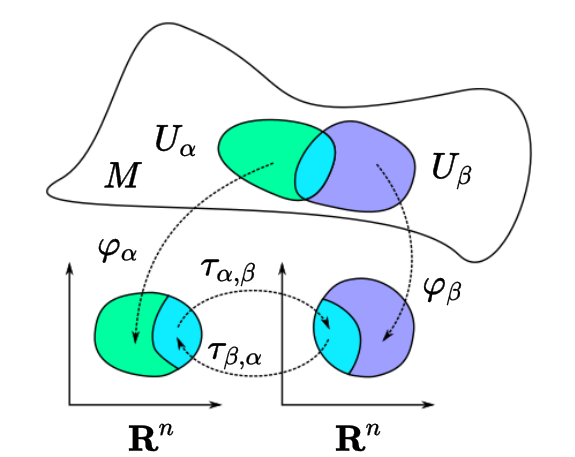
\includegraphics[width=0.5\textwidth]{1.png}
        \caption{Illustration of the transition map for real manifolds. For our situations, just set $n=2$ and identify $\real^2$ with $\cx$ in the usual way. From \url{https://www.bookofproofs.org/branches/transition-map/}.}
        \label{fig:Fig1}
    \end{figure}
\end{definition}
\begin{exercise}
    \noindent
    \begin{enumerate}[(a)]
        \item Show that the definition of compatible charts is symmetric.
        \item Show that compatibility is $\ita{not}$ transitive.
    \end{enumerate}
\end{exercise}
\begin{example}
    Any two charts on open sets of $\real^2$ of the form $(x,y)\mapsto x+iy$ are compatible, and similarly for $(x,y)\mapsto x-iy$. However, the maps $(x,y)\mapsto x+iy$ and $(x,y)\mapsto x-iy$ are \ita{not} compatible, as complex conjugation is not analytic.
\end{example}
\begin{exercise}
    Let $U_1,U_2\subseteq\cx$ be open, $\phi_j:U_j\to U_j^*$ conjugate maps. Show that $\phi_1,\phi_2$ are compatible.
\end{exercise}
\begin{example}
    Any two subcharts of a chart are compatible.
\end{example}
\begin{exercise}
    Consider the unit sphere $S^2\subset\real^3$, $N=(0,0,1)$, $P=(0,0,-1)$. Show that the projections $\phi_1:S^2\setminus N\to\cx$, $\phi_2:S^2\setminus P\to\cx$ are \ita{not} compatible, but $\phi_1$ and $\overline{\phi_2}$ \ita{are} ($\overline{\phi_2}(x,y,z):=\overline{\phi_2(x,y,z)}$).
\end{exercise}
\section{January 27}
\subsection{More From Last Time}
Recall: let $X$ be a topological space. A \underline{chart} on $X$ is a homeomorphism $\varphi:U\to V$ where $U\subseteq X$ and $V\subseteq\cx$ are open. Two charts are \underline{compatible} if their transition map is a biholomorphism ($f:U\to V$ is a \textbf{biholomorphism} if it is an analytic bijection with analytic inverse.)
\begin{definition}
    Let $X$ be a topological space. An \textbf{atlas} $\mathcal{A}$ is a collection $\mathcal{A}=\{\varphi_{\alpha}:U_{\alpha}\to V_{\alpha}\}_{\alpha\in J}$ such that the collection $\{U_{\alpha}\}_{\alpha\in J}$ covers $X$ (so $\bigcup\limits_{\alpha\in J}U_{\alpha}=X$) and the $\varphi_{\alpha}$'s are pairwise compatible charts.
    
    Two atlases $\mathcal{A},\mathcal{B}$ are \textbf{compatible} if all of the charts of $\mathcal{A}$ and $\mathcal{B}$ are compatible; equivalently if $\mathcal{A}\cup\mathcal{B}$ is an atlas.
    
    An atlas $\mathcal{A}$ is \textbf{maximal} if it is not properly contained in any other atlas.
\end{definition}
\begin{example}
    $\real^2$ has the one chart atlas $\phi:(x,y)\mapsto x+iy$. The conjugate of this map is also a one chart atlas, but these two atlases are not compatible.
\end{example}
\begin{exercise}
    Show that compatibility of atlases \ita{is} an equivalence relation.
\end{exercise}
\begin{exercise}
    Let $X$ be a topological space, $\mathcal{A}$ an atlas on $X$.
    \begin{enumerate}[(a)]
        \item Use Zorn's Lemma to show that $\mathcal{A}$ is contained in a maximal atlas.
        \item Show that this maximal atlas containing $\mathcal{A}$ is unique.
    \end{enumerate}
\end{exercise}
\subsection{Digression on Zorn's Lemma}
Let $(S,\preceq)$ be a partially ordered set with the property that every \underline{chain} (totally ordered subset) has an upper bound. Then $S$ has maximal elements.

As an example, we prove that every vector space has a basis. 
\begin{claim}
    Let $V$ be a vector space over a field $k$. Then $V$ has a basis.
\end{claim}
\begin{proof}
    Let $S$ be the set of all linearly independent subsets of $V$. Let $\mathcal{C}$ be a chain in $S$ with respect to $\subseteq$. Let 
    \begin{equation}
        T=\bigcup\limits_{C\in\mathcal{C}}C.
    \end{equation}
    Clearly $C\subseteq T$ for all $C\in\mathcal{C}$. Suppose that $T$ is not linearly independent. Then there exists $v_1,\dotsc,v_n\in T$, $a_1,\dotsc,a_n\in k$ not all zero such that $a_1v_1+\dotsb+a_nv_n=0$. Then there is some $C\in\mathcal{C}$ containing all of these $v_j$'s. But then $C$ is not linearly independent, a contradiction. Hence $T$ must be linearly independent, and therefore every chain of linearly independent sets has an upper bound. Thus by Zorn's Lemma, so $X$ has a maximal linearly independent set $W$. We claim that $V=\mathrm{span}_kW$. Otherwise there exists $y\in V$ such that $y\notin\mathrm{span}_kW$, so $y\notin W$. Hence $W\cup\{y\}$ is linearly dependent. Then there exists $w_1,\dotsc,w_n\in W$, $a_1,\dotsc,a_n,b\in k$ not all zero such that $a_1w_1+\dotsb+a_nw_n+by=0$. Note that $b\neq0$, otherwise $w_1,\dotsc,w_n$ are linearly dependent. Thus 
    \begin{equation}
        y=-\frac{1}{b}(a_1w_1+\dotsb+a_nw_n),
    \end{equation}
    so $y\in\mathrm{span}_kW$, a contradiction. Therefore $W$ is indeed a basis for $V$.
\end{proof}

\subsection{Riemann Surface Introduction}
\begin{definition}
    Let $X$ be a topological space. A \textbf{complex structure} (or conformal structure) on $X$ is a maximal atlas on $X$.
\end{definition}
\begin{definition}
    A \textbf{Riemann surface} is a connected, Hausdorff, second countable topological space with a complex structure.
\end{definition}
\begin{remark}
    \noindent
    \begin{itemize}
        \item Some do \ita{not} insist that a Riemann surface be connected. We will require them to be.
        \item \underline{Hausdorff} means any two distinct points have disjoint open neighborhoods. Why do we need this? The plane with two origins $\cx\cup\{0_a\}$ satisfies all of these requirements \ita{except} Hausdorff.
        \item \underline{Second countable} means that $X$ has a countable base for its topology. An example of a non-second countable space is the long line.
    \end{itemize}
\end{remark}
\begin{example}
    \noindent
    \begin{itemize}
        \item $\cx$ and any connected open subset of $\cx$ are clearly Riemann surfaces.
        \item $S^2$ with the two compatible charts is a Riemann surface. Here, we think of $S^2$ as the Riemann sphere.
        \item In general, given a Riemann surface and a ``nice enough'' action of a group on it, the orbits* form a Riemann surface. By nice enough, we mean that the orbits are discrete. If $G$ is a discrete subgroup of $\cx$, then the quotient group $\cx/G$ can be made into a Riemann surface.
        
        *Recall that if $G$ acts on a set $X$, the orbit $\mathcal{O}_x$ containing $x\in X$ is the subset of $X$ given by 
        \[\mathcal{O}_x=\{g\cdot x\mid g\in G\}.\]
        The orbits form a partition of $X$.
        
        Let's consider finitely generated (additive) subgroups of $\cx$. Any finitely generated subgroup of $\cx$ is isomorphic to 
        \begin{equation}
            \bigoplus\limits_{j=1}^n\z=\z^n
        \end{equation}
        for some $n\in\z^+$. $n$ is called the \textbf{rank}.
        
        As a pre-example, consider $\z<\real$. Then $\real/\z$ has a complete set of coset representatives given by $[0,1)$, and $\real/\z\cong S^1$. In general, such a complete set of coset representatives is called a \textbf{fundamental domain}.
        
        Similarly, if $G$ is a cyclic subgroup of $\cx$, $\cx/G$ is a cylinder, which is a Riemann surface. Now consider $G=\vbrack{\omega_1,\omega_2}$, where $\omega_1,\omega_2\in\cx$ are linearly dependent over $\real$ (also assume that both are nonzero). So $\omega_2=\lambda\omega_1$ for some $\lambda\in\real\setminus\{0\}$. If $\lambda\in\q$, say $\lambda=\frac{p}{q}$ for $p,q\in\z\setminus\{0\}$, $\gcd(p,q)=1$, then there exists $m,n\in\z$ such that $pm+qn=1$. Stay tuned for next time!
    \end{itemize}
\end{example}
\section{January 29}
\subsection{More From Last Time}
$G$ is a 2-generated subgroup of $\cx$, say $G=\z\omega_1+\z\omega_2$. If $\omega_2=\frac{p}{q}\omega_1$ for some $p,q\in\z$ ($q\neq0$), $\gcd(p,q)=1$, then there exists $m,n\in\z$ such that $mp+nq=1$. Then $nq\omega_2=np\omega_1$, so 
\begin{equation}
    \begin{split}
        n\omega_1+m\omega_2&=\left(1+\frac{mp}{q}\right)\omega_1\\
        &=\frac{nq+mp}{q}\omega_1\\
        &=\frac{1}{q}\omega_1\in G.
    \end{split}
\end{equation}
Hence $\z\omega_1+\z\omega_2=\z\omega_1$, so $G$ is cyclic.

If $\omega_2$ is an \underline{irrational multiple} of $\omega_1$, say $\alpha$, then by Dirichlet's Approximation Theorem there are infinitely many rational numbers $\frac{p}{q}$ such that $\left|\alpha-\frac{p}{q}\right|<\frac{1}{q^2}$. For each $p,q$, $|q\alpha-p|<\frac{1}{q}$ and $(q\alpha-p)\omega_1\in G$. So 0 is an accumulation point of $G$, which we don't want!

If $\omega_1$ and $\omega_2$ are \underline{linearly independent} over $\real$, we get a discrete group, a \textbf{Bravais lattice}!
\begin{figure}[H]
    \centering
    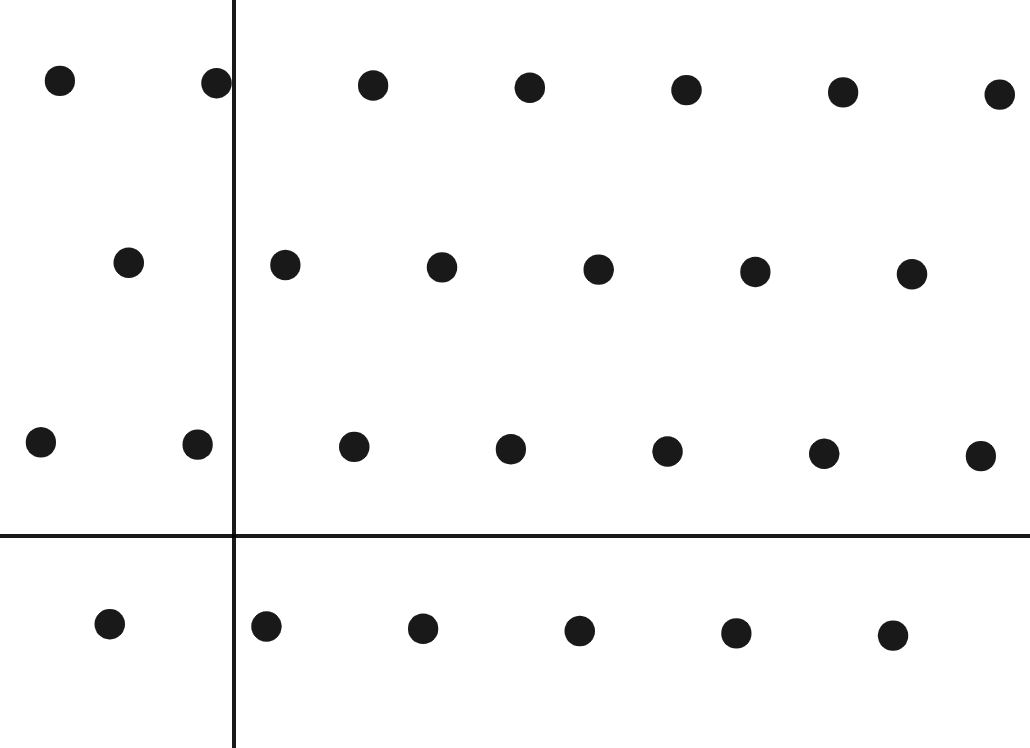
\includegraphics[width=0.5\textwidth]{2.png}
    \caption{$G$ for $\omega_1$, $\omega_2$ linearly independent over $\real$. From \url{https://www.desmos.com/calculator/cs33ymjbsl}.}
    \label{fig:Fig2}
\end{figure}
A fundamental domain for $X=\cx/G$ is the parallelogram formed by $\omega_1$ and $\omega_2$. $X$ is a torus (topologically), and we will discuss complex tori later. 
Now, is $X$ a Riemann surface? Yes, the topology on $X$ is given by the quotient map by the projection, so the quotient homomorphism $\cx\to\cx/G$ is also the quotient map for the quotient topology. So connectedness is preserved. Is it second countable? Yes: as a topological space $X \cong S^1 \times S^1$, and as $S^1$ is second countable, so is the product. Is it Hausdorff? Yes, since $G$ is discrete, which is why we wanted $G$ to be discrete in the first place! 

Also, $X$ is the image of the closure of its fundamental domain, which makes it compact!
\subsection{Example: \texorpdfstring{$\p^1$}{P1}}
Let's starts with $\p_{\real}^1=\mathbb{RP}^1=\{(x,y)\in\real^2\setminus\{(0,0)\}\}/\sim$, where $(x_1,y_1)\sim(x_2,y_2)$ if there exists $\lambda\in\real^*$ (for a ring $R$, $R^*$ is the group of units, and for a field $k$, $k^*=k\setminus\{0\}$), such that $x_1=\lambda y_1$ and $x_2=\lambda y_2$. This is actually $S^1$: one way to visualize it is to identify antipodal points on $S^1$. Then we get a semicircle, with the two endpoints identified. This gets us back to a circle!

In general, for a field $k$, consider the vector space $k^{n+1}$. Define an equivalence relation $\sim$ on $k^{n+1}\setminus\{(0,\dotsc,0)\}$ (where $(0,\dotsc,0)$ is the zero vector) by $x\sim y$ if there exists $\lambda\in k^*$ such that $x=\lambda y$. Then the $n$-dimensional projective space over $k$ is defined as
\begin{equation}
    \p_k^n:=\left(k^{n+1}\setminus\{(0,\dotsc,0)\}\right)\big/\sim.
\end{equation}
$\p_k^n$ is the set of all 1-dimensional subspaces of $k^{n+1}$.

Now, let's look at $\p_{\cx}^1=\mathbb{CP}^1=\left(\cx^2\setminus\{(0,0)\}\right)\big/\sim$ (for convenience let's just write $\p^1$ from here on out). $\p$ has a \textbf{projective coordinate system} $[z,w]$ for equivalence classes of $(z,w)$. So for example, $[1,2]=[2,4]$. 

This equivalence raises all sorts of issues, however. For example, $(2,4)$ satisfies $z=w^2$ but $(1,2)$ does not. Furthermore, for any $\lambda\in\cx^*$, any non-negative integers $a\leq n$, and any $z,w\in\cx$
\begin{equation}
    (\lambda z)^a(\lambda w)^{n-a}=\lambda^nz^aw^{n-a}.
\end{equation}
So if $F(z,w)$ is a homogeneous polynomial* of degree $n$, $F(\lambda z,\lambda w)=\lambda^nF(z,w)$. So in general $F[z,w]$ is not a well-defined function, but where it vanishes is! 

*$F\in k[x_1,x_2,\dotsc,x_n,x_{n+1}]$ is a \textbf{homogeneous polynomial of degree $d$} if every monomial term of $F$ has degree $d$.

Further, if $F$ and $G$ are homogeneous of the same degree $n$ and $G$ is not the zero polynomial, the rational function $\frac{F}{G}$ is well-defined on projective coordinates, at least where $G$ is nonzero. This is because
\begin{equation}
    \frac{F(\lambda z,\lambda w)}{G(\lambda z,\lambda w)}=\frac{\lambda^n F(z,w)}{\lambda^n G(z,w)}=\frac{F(z,w)}{G(z,w)}.\,\checkmark
\end{equation}
To give $\p^1$ a complex structure, notice that $\cx$ maps bijectively to $\{[z,1]\mid z \in\cx\}=\p^1\setminus\{[1,0]\}$, since if $w\neq0$, then $[z,w]=\left[\frac{z}{w},1\right]$. Similarly $\cx\xlongrightarrow{\sim}\{[1,w]\mid w\in\cx\}=\p^1\setminus\{[0,1]\}$. The inverses of these maps we take to be the charts, and on the overlap, we have
\begin{equation}
    z\mapsto[z,1]=\left[1,\frac{1}{z}\right]\mapsto\frac{1}{z}.
\end{equation}
Since 0 is not included in the overlap, we get an analytic function!

$\p^1$ is \underline{Hausdorff}: if two points are in the same chart, then they can be separated. On the other hand, $\{[z,1]\mid|z|<1\}$ and $\{[1,w]\mid|w|<1\}$ are disjoint neighborhoods of $[0,1]$ and $[1,0]$, thus every pair of distinct points have disjoint neighborhoods. Furthermore, $\p^1$ is a compact Riemann surface.

Just what does this guy look like? Think of $S^2$...
\subsection{Implicit Function Theorem}
Let $U\subseteq\cx$ be open (and connected?), and let $F:U\to\cx$ be an analytic function. Then the graph $C:=\{(z,w)\in\cx^2\mid w=F(z)\}$ is a Riemann surface. The projection map $\pi:C\to\cx$, $z\mapsto z$ is a one-chart atlas.

More generally, let $F$ be a function of \ita{two} complex variables. We want to study the set $\{(z,w)\in\cx^2\mid F(z,w)=0\}$. This set is usually not a manifold! Even in the real case, we have problems. In $\real^2$, let $F(x,y):=x^3+y^3-3xy$. The zero set of this function forms an algebraic curve called the \underline{folium of Descartes}. 
\begin{figure}[H]
    \centering
    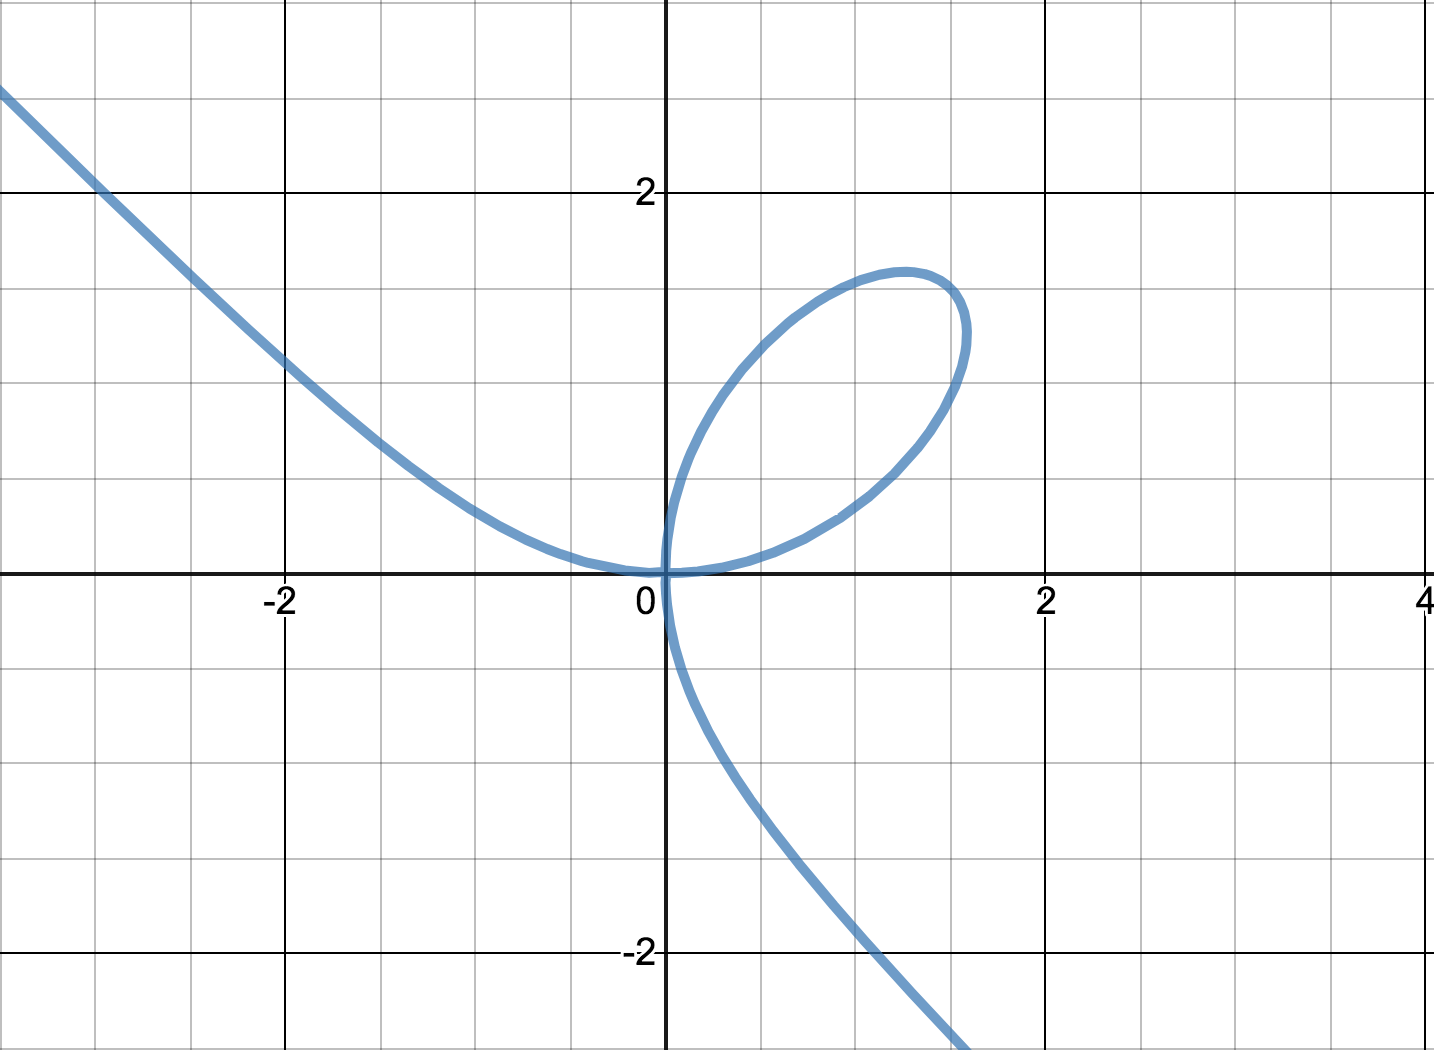
\includegraphics[width=0.5\textwidth]{3.png}
    \caption{Graph of the zero set of $F(x,y)$ as given above. Plotted in \cite{Desmos}.}
    \label{fig:Fig3}
\end{figure}
The zero set of $F$ is definitely not locally Euclidean at $(0,0)$!

Take the following example:
\begin{figure}[H]
    \centering
    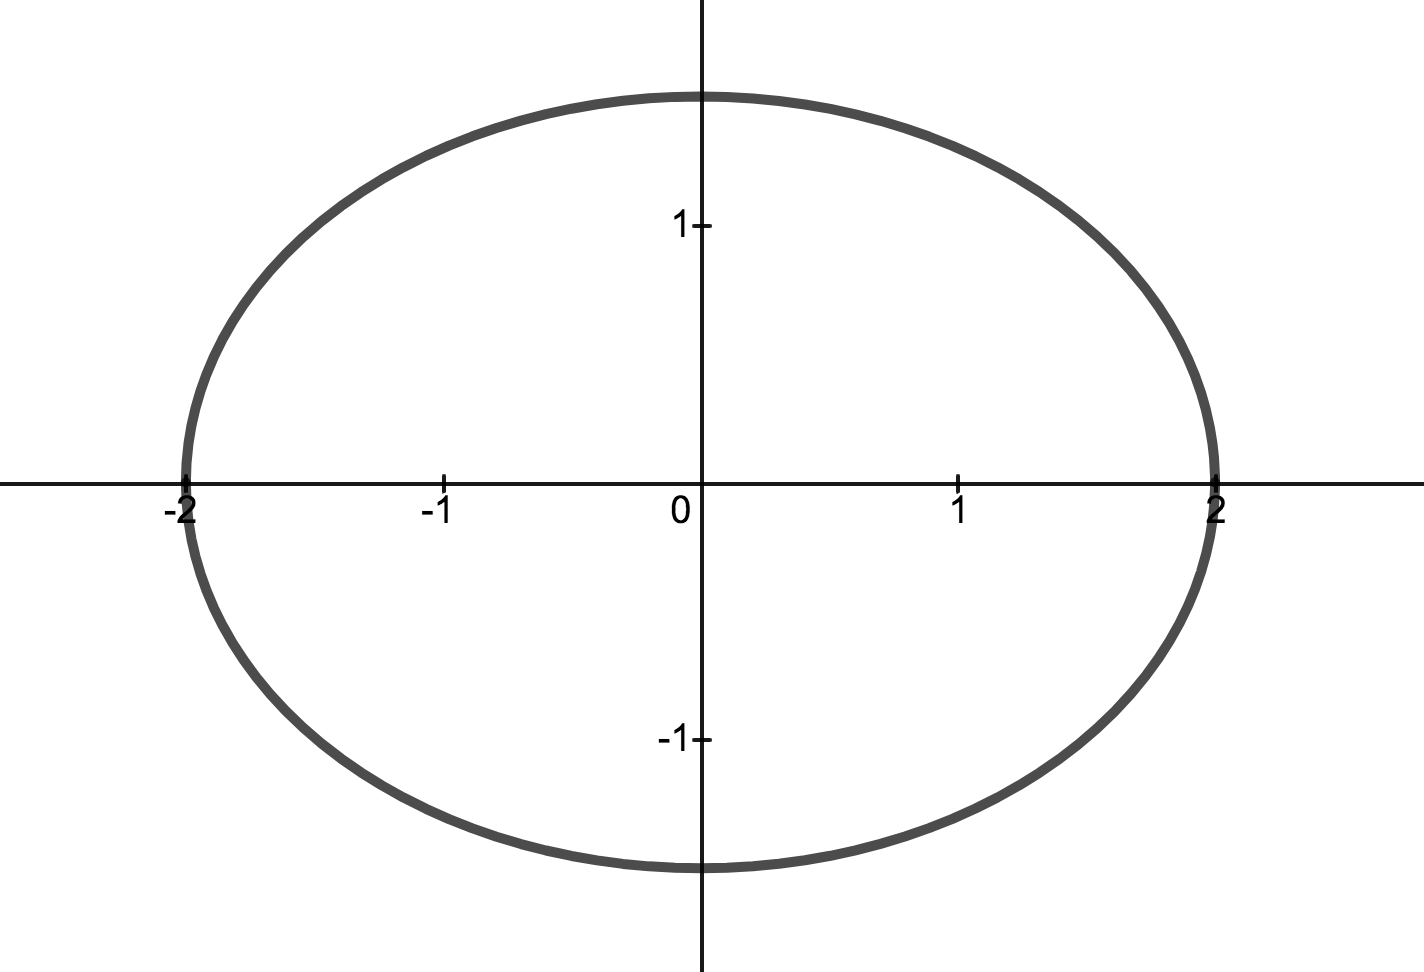
\includegraphics[width=0.5\textwidth]{4.png}
    \caption{Graph of the zero set of $F(x,y):=9x^2+16y^2-36$. As $F$ is just a polynomial in two variables, it is smooth. Plotted in Desmos.}
    \label{fig:Fig4}
\end{figure}
Locally, this looks like the graph of a smooth function, so we can try to patch up the entire thing with coordinate charts.
\begin{figure}[H]
    \centering
    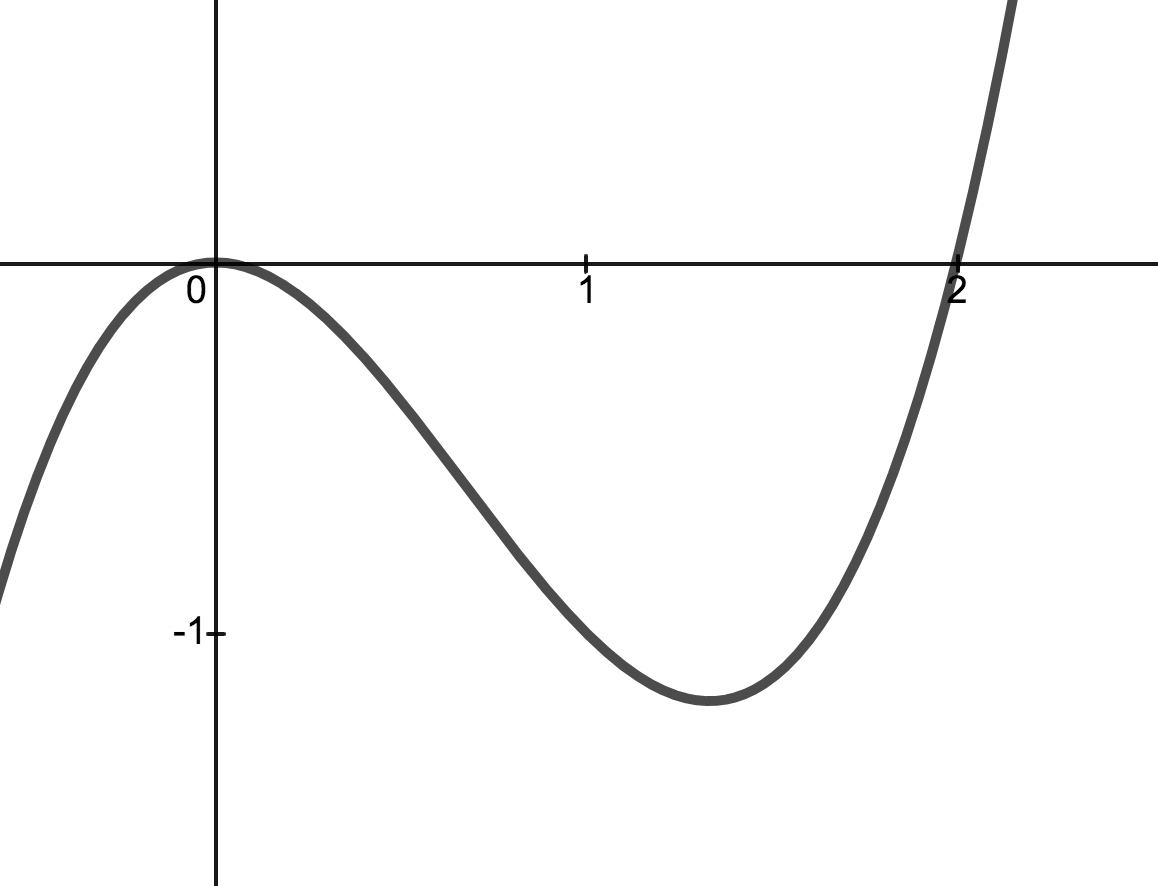
\includegraphics[width=0.5\textwidth]{5.png}
    \caption{Graph of the function $f(x):=x^3-2x^2$. On the intervals where $f$ is monotone, the graph of $f$ can also be made into a function of $y$. Plotted in \cite{Desmos}.}
    \label{fig:Fig5}
\end{figure}
If we look at a smooth function $f:\real\to\real$, we can locally make its graph a function of $y$ as well, but only where $f'\neq0$, else we don't get a function.

We want something like an \underline{Implicit Function Theorem}!
\begin{theorem}
    Let $F$ be a function of two complex variables and suppose $F(z,w)$ is continuous and analytic in each variable separately, defined on some open region $W\subseteq\cx^2$. Suppose there exists $(z_0,w_0)\in W$ such that $F(z_0,w_0)=0$ and $F_2(z_0,w_0):=\frac{\partial}{\partial w}F(z_0,w_0)\neq0$. Then there are open neighborhoods $U$ of $z_0$, $V$ of $w_0$ such that for each $z\in U$, there is a unique $w\in V$ such that $F(z,w)=0$. This defines $w$ as a function $w=g(z)$ on $U$. Then $g$ is analytic on $U$, and its derivative is given by the formula... next time!
\end{theorem}
Similarly, we can do the same for when $F_1(z_0,w_0):=\frac{\partial}{\partial z}F(z_0,w_0)\neq0$. 
\begin{exercise}
    Prove the real-variables version of Implicit Function Theorem stated in class: let $W\subseteq\real^2$ be open, and $F:W\to\real$ be continuously differentiable. Suppose there exists $(x_0,y_0)\in W$ such that $F(x_0,y_0)=0$ and $F_2(x_0,y_0):=\frac{\partial}{\partial y}F(x_0,y_0)\neq0$. Then there exists open neighborhoods $U$ of $x_0$, $V$ of $y_0$ such that for each $x\in U$, there is a unique $y\in V$ such that $F(x,y)=0$. This defines $y$ as a continuously differentiable function $y=g(x)$ on $U$.
\end{exercise}
\section{February 3}
\subsection{Some More Complex Analysis}
Suppose $f$ is analytic on some open disk $D$ and its boundary $\partial D$, and suppose $f$ has a zero of order $n$ at some point $z_0\in D$. Locally, $f$ has a power series expansion
\begin{equation}
    f(z)=a_n(z-z_0)^n+a_{n+1}(z-z_0)^{n+1}+\dotsb
\end{equation}
where $a_n\neq0$, and its derivative $f'$ has a power series expansion
\begin{equation}
    f'(z)=na_n(z-z_0)^{n-1}+(n-1)a_{n+1}(z-z_0)^{n-2}+\dotsb
\end{equation}
Thus we can write
\begin{equation}
    \frac{f'(z)}{f(z)}=\frac{na_n(z-z_0)^{n-1}\left[1+\frac{(n-1)a_{n+1}}{na_n}(z-z_0)+\dotsb\right]}{a_n(z-z_0)^n\left[1+\frac{a_{n+1}}{a_n}(z-z_0)+\dotsb\right]}=\frac{n}{z-z_0}g(z)
\end{equation}
where $g$ is analytic in a neighborhood of $z_0$, and $g(z_0)=1$. Then $\frac{f'}{f}$ has residue $n$ at $z_0$. Now, if $z_0$ was instead a \ita{pole} of order $m$, then the residue of $\frac{f'}{f}$ at $z_0$ can be computed similarly, which gives us $-m$.

So if $f$ has zeroes $\{z_j\mid1\leq j\leq N\}$ of orders $n_j$ and poles $\{p_k\mid1\leq k\leq M\}$ of orders $m_k$ in $D$ (none lying on the boundary), then 
\begin{equation}
    \frac{1}{2\pi i}\int_{\gamma}\frac{f'(z)}{f(z)}\,\mathrm{d}z=\sum\limits_{j=1}^Nn_j-\sum\limits_{k=1}^Mm_k,
\end{equation}
where $\gamma:[0,2\pi]\to\cx$, $\gamma(s):=z_0+re^{is}$, $0\leq s\leq2\pi$ is the boundary curve for $\partial D$ ($r$ is the radius of $D$). 
\begin{exercise}
    In the setting above, let $g$ be analytic on a neighborhood of $D\cup\partial D$. Show that 
    \begin{equation}
        \frac{1}{2\pi i}\int_{\gamma}g(z)\frac{f'(z)}{f(z)}\,\mathrm{d}z=\sum\limits_{j=1}^Nn_jg(z_j)-\sum\limits_{k=1}^Mm_kg(p_k).
    \end{equation}
    In particular, if $f$ has a simple zero $z_0$ and no poles, then 
    \begin{equation}
        \frac{1}{2\pi i}\int_{\gamma}\frac{zf'(z)}{f(z)}\,\mathrm{d}z=z_0.
    \end{equation}
\end{exercise}
This is called the \textbf{Argument Principle}, so called since 
\begin{equation}
    \frac{1}{2\pi i}\int_{\gamma}\frac{f'(z)}{f(z)}\,\mathrm{d}z=\frac{1}{2\pi i}\int_{f\circ\gamma}\frac{\,\mathrm{d}z}{z}=n(f\circ\gamma;0),
\end{equation}
the winding number of $f\circ\gamma$ about the origin.
\begin{theorem}[Rouch\'e's Theorem]
    Suppose that $f$ and $g$ are analytic in some neighborhood of $D$ with boundary $\partial D$ such that $\partial D$ contains no zeros of either function. Suppose further that for all $z\in\partial D$, $|f(z)-g(z)|<|f(z)|$. Then $f$ and $g$ have the same number of zeros counted with multiplicity in $D$. In fact, this is remains true under the hypothesis that $|f(z)-g(z)|<|f(z)|+|g(z)|$ on $\partial D$.
\end{theorem}
\begin{proof}
    This weaker hypothesis is only false if $g(z)$ is a non-positive (and hence real) scalar multiple of $f(z)$ for some $z\in\partial D$. Otherwise $\Log\left(\frac{f}{g}\right)$ is defined on a neighborhood of $\partial D$, where $\Log$ is the principal branch of the logarithm. In any small neighborhood where $\log(f)$ and $\log(g)$ are defined on the same branch, $\log\left(\frac{f}{g}\right)=\log(f)-\log(g)$ is analytic, with derivative $\frac{f'}{f}-\frac{g'}{g}$. Thus $\frac{f'}{f}-\frac{g'}{g}$ has a primitive in a neighborhood of $\partial D$, and so by Cauchy's theorem,
    \begin{equation}
        \frac{1}{2\pi i}\int_{\gamma}\left[\frac{f'(z)}{f(z)}-\frac{g'(z)}{g(z)}\right]\,\mathrm{d}z=0,
    \end{equation}
    and thus
    \begin{equation}
        \frac{1}{2\pi i}\int_{\gamma}\frac{f'(z)}{f(z)}\,\mathrm{d}z=\frac{1}{2\pi i}\int_{\gamma}\frac{g'(z)}{g(z)}\,\mathrm{d}z.
    \end{equation}
    Alternatively, take the straight line homotopy between $f\circ\gamma$ and $g\circ\gamma$:
    \begin{equation}
        \mu(s,t):=(1-t)(f\circ\gamma)(s)+t(g\circ\gamma)(s).
    \end{equation}
    Furthermore, this homotopy is never zero, else $f$ and $g$ are nonpositive scalar multiples of each other. Hence $\frac{1}{2\pi i}\int_{\mu(\cdot,t)}\frac{\,\mathrm{d}z}{z}$ is integer-valued and continuous in $t$, and so it is constant. Therefore the number of zeros of $f$ in $D$ counted with multiplicity is 
    \begin{equation}
        \frac{1}{2\pi i}\int_{f\circ\gamma}\frac{\,\mathrm{d}z}{z}=\frac{1}{2\pi i}\int_{g\circ\gamma}\frac{\,\mathrm{d}z}{z},
    \end{equation}
    which is the number of zeros of $g$ in $D$ counted with multiplicity.
\end{proof}
\subsection{Implicit Function Theorem}
Finally we'll prove this!
\begin{theorem}[Implicit Function Theorem]
    Let $W\subseteq\cx\times\cx$ be open and connected, and let $F:W\to\cx$ be continuous and also analytic in each variable separately. Suppose that there exists $(z_0,w_0)\in W$ such that $F(z_0,w_0)=0$ and $F_2(z_0,w_0)\neq0$. Then there exists open neighborhoods $U$, $V$ of $z_0$, $w_0$, respectively, such that for each $z\in U$, there is a unique $w\in V$ such that $F(z,w)=0$. The function $w=g(z)$ so defined is analytic in a neighborhood of $z_0$.
\end{theorem}
\begin{proof}
    Treat $F(z_0,\cdot)$ as a function of one complex variable. Then as its zeros are isolated there exists $\rho>0$ such that $w_0$ is the only zero in $D:=\overline{B(w_0;\rho)}$. Since the boundary $C$ of $D$ is compact ($C=\partial D\cong S^1$), $|F(z_0,\cdot)|$ attains its strictly positive minimum on $C$, so $|F(z_0,w)|\geq m>0$ for all $w\in C$. On the other hand, for each $w_1\in D$ there exists $\epsilon_{w_1},\delta_{w_1}>0$ such that for all $z\in B(z_0;\epsilon_{w_1})$ and $w\in B(w_0;\delta_{w_1})$, $|F(z,w)-F(z,w_1)|<\frac{m}{4}$. Since $D$ is compact, a finite number of the $B(w_1;\delta_{w_1})'s$ cover $D$; let $\epsilon>0$ be the minimum of the corresponding $\epsilon_{w_1}$'s. Then for all $w\in D$, $z\in B(z_0;\epsilon)$, 
    \begin{equation}
        |F(z,w)-F(z_0,w_1)|\leq\dotsb
    \end{equation}
\end{proof}
\section{February 5}
\subsection{Implicit Function Theorem (cont'd)}
Let's get this done with!
\begin{proof}[Proof of Implicit Function Theorem]
    $F(z_0,\cdot)$ has isolated zeros, so there exists $\rho>0$ such that $D:=\overline{B(w_0;\rho)}$ contains no other zeros of $F(z_0,w)$. Then $|F(z_0,w)|$ reaches a minimum on $C:=\partial D$, say $m>0$. For each $w_1\in D$ there exists $\epsilon_{w_1},\delta_{w_1}>0$ such that for all $(z,w)\in B(z_0;\epsilon_{w_1})\times B(w_1;\delta_{w_1})$,
    \begin{equation}
        |F(z,w)-F(z,w_1)|<\frac{m}{2}.
    \end{equation}
    $D$ is compact, so it is covered by finitely many of the $B(w_1;\delta_{w_1})$'s, say $U_j:=B(w_{1_j};\delta_{w_{1_j}})$ for $j\in\oneton$. Let $\epsilon:=\min\{\epsilon_{w_{1_j}}\mid1\leq j\leq n\}$. Now the collection $\{B(z_0;\epsilon)\times U_j\mid1\leq j\leq n\}$ covers $B(z_0;\epsilon)\times D$. For all $w\in D$, $z\in B(z_0;\epsilon)$, $w$ lies in some $U_j$, and so $(z,w)$ lies in $B(z_0;\epsilon)\times U_j$, and so does $(z_0,w)$. So 
    \begin{equation}
        \begin{split}
            |F(z,w)-F(z_0,w)|&\leq|F(z,w)-F(z,w_{1_j})|+|F(z,w_{1_j})-F(z_0,w_{1_j})|\\
            &<\frac{m}{2}+\frac{m}{2}=m.
        \end{split}
    \end{equation}
    For any $w\in C$, $|F(z_0,w)-F(z_1,w)|<m$ and $|F(z_0,w)|\geq m$. By Rouch\'e's Theorem, $F(z,w)$ has exactly one root on $C$. Call this $w_1$. By Exercise 10 applied to the function $F(z_1,w)$, 
    \begin{equation}
        \frac{1}{2\pi i}\int_Cw\frac{F_2(z_1,w)}{F(z_1,w)}\,\mathrm{d}w=w_1.
    \end{equation}
    So the $w$ for which $F(z,w)=0$ is given by 
    \begin{equation}
        g(z)=\frac{1}{2\pi i}\int_C\frac{wF_2(z,w)}{F(z,w)}\,\mathrm{d}w.
    \end{equation}
    Hence $g$ is analytic.
\end{proof}
\begin{exercise}
    Apply Rouch\'e's Theorem in a similar way to the above proof to prove the Open Mapping Theorem. (Use functions of the form $f(z)-w_0$ and $f(z)-w$ for $w$ close enough to $w_0$).
\end{exercise}
\begin{exercise}
    Use Implicit Function Theorem to prove the Inverse Function Theorem: Let $f$ be analytic on the same open set containing $z_0$ such that $f'(z_0)\neq0$. Then there is a neighborhood $U$ of $z_0$ and a neighborhood $V$ of $f(z_0)$ such that $f$ has an analytic inverse $\inv{f}:V\to U$.
\end{exercise}
\begin{exercise}
    Let $F$ be a continuous function of 2 variables separately defined on some open set in $\cx^2$. Let $C:=\{(z,w)\in\cx^2\mid F(z,w)=0\}$, and suppose that at each point $(z,w)$ on $C$, either $F_1(z,w)\neq0$ or $F_2(z,w)\neq0$. Show that either $z$ or $w$ gives a chart at each point $C$ and that these form an atlas. Conclude that $C$ is a Riemann surface.
\end{exercise}
\subsection{Affine Plane Curves}
Now let $F$ be a polynomial in two variables (so $F\in\cx[z,w]$), and let $V(F)\subseteq\cx^2$ be its vanishing set:
\begin{equation}
    V(F):=\{(z,w)\mid F(z,w)=0\}.
\end{equation}
$V(F)$ is called an \textbf{affine plane curve}.
\begin{example}
    The real part of $V(z^2-w)$ is the familiar parabola in the plane. Rather, what we can understand is $V(x^2-y)$ where $x$ and $y$ are real variables. Since we can't actually plot these in two dimensions, we plot them in $\real^2$ as the vanishing set of polynomials in two real variables. Keep that in mind; any plots we include moving forward are not showing the full picture.
    \begin{figure}[H]
        \centering
        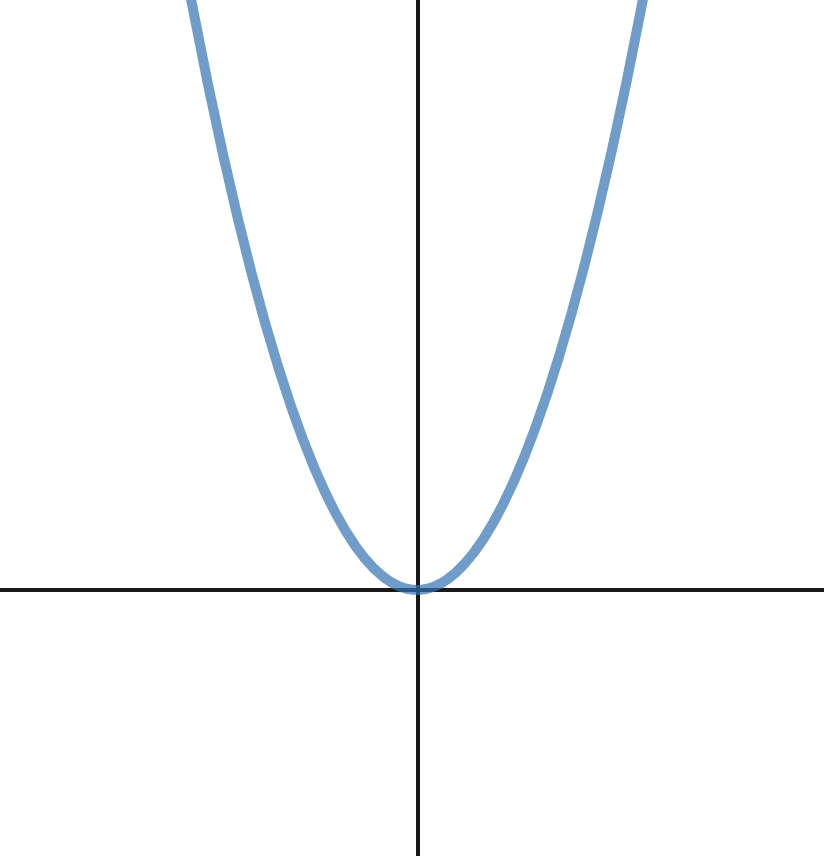
\includegraphics[width=0.5\textwidth]{6.png}
        \caption{Real part of $V(z^2-w)$.}
        \label{fig:Fig6}
    \end{figure}
\end{example}
If each point has one nonvanishing partial derivative of $F$, then $V(F)$ is a Riemann surface by Exercise 13. Such a curve is called \textbf{nonsingular}. A singular point on a curve is a point where both partial derivatives vanish, provided $F$ is \underline{squarefree}.
\begin{definition}
    Let $R$ be a Unique Factorization Domain (UFD). $r\in R$ is \textbf{squarefree} if no repeated terms appear in its factorization.
\end{definition}
(Recall that $\cx[z,w]$ is a UFD). Why do we want squarefree polynomials? 
\begin{example}
    Note that $V(z^2)=V(z)$. This is because for $F(z,w):=z^2$, $F_1=F_2=0$ on $V(z)$, so $F$ is singular everywhere on $V(z)$. However, $G(z,w):=z$ is nonsingular \ita{everywhere}.
\end{example}
The degree of an affine plane curve $C=V(F)$ is just $\deg(F)$, the total degree in $z$ and $w$. As practice, what is the degree of the following?
\begin{equation}
    F=z^4w^2+z^5-4w^2+zw
\end{equation}
$F$ has degree 6, since the $z^4w^2$ term contributes total degree 6. 
\begin{example}
    \noindent
    \begin{itemize}
        \item $C=V(zw)=V(z)\cup V(w)$. Treating $\cx^2$ as $\real^4$, this consists of two planes intersecting at the origin. The intersection point at the origin is a singular point, so $C$ is not a Riemann surface.
        \item $C=V((z-w)(z-w+1))=V(z-w)\cup V(z-w+1)$ consists of two parallel complex lines, and so in $\real^4$ would be two parallel planes, with one passing through the origin. While both pieces are themselves Riemann surfaces, $C$ itself is not since it is not \underline{connected}.
    \end{itemize}
    \begin{figure}[H]
        \begin{subfigure}{0.5\textwidth}
            \centering
            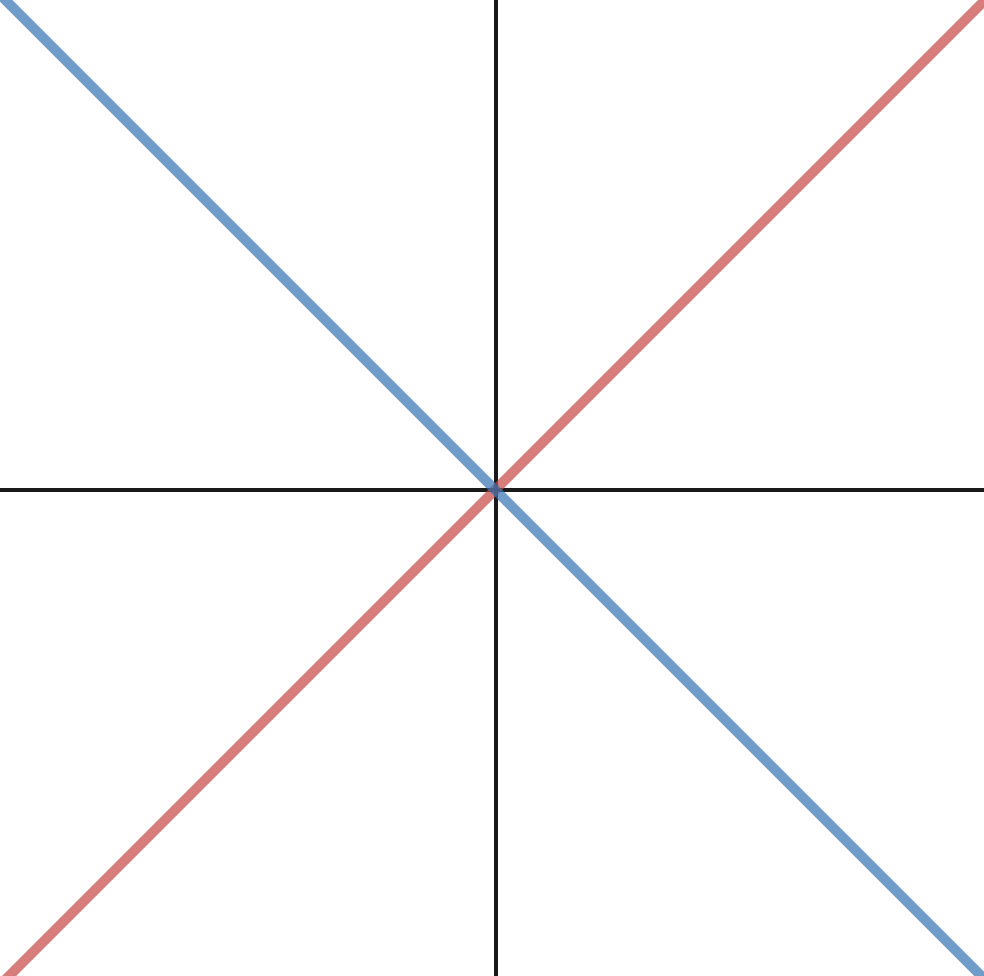
\includegraphics[width=0.5\textwidth]{7.png}
            \caption{$V(zw)$.}
            \label{fig:subim1}
        \end{subfigure}
        \begin{subfigure}{0.5\textwidth}
            \centering
            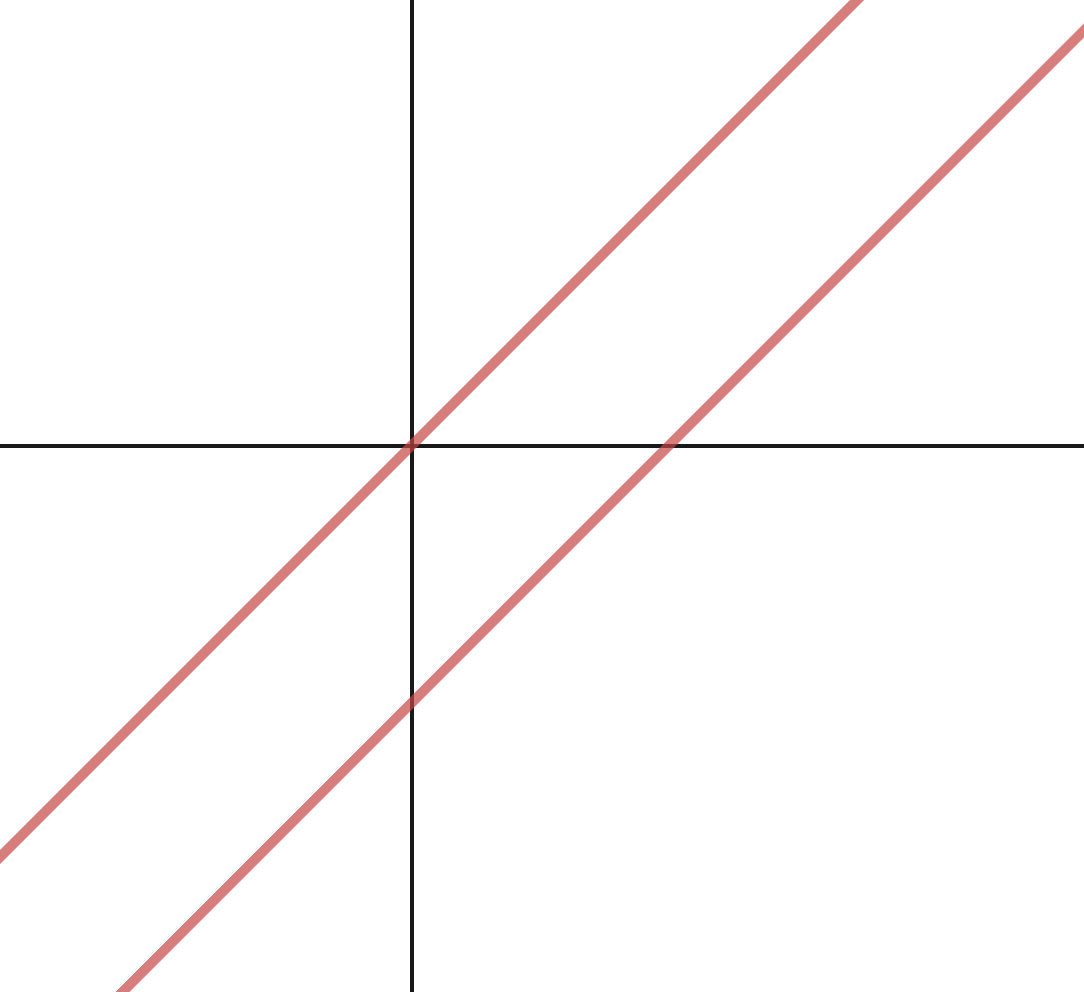
\includegraphics[width=0.5\textwidth]{8.png}
            \caption{$V((z-w)(z-w+1))$.}
            \label{fig:subim2}
        \end{subfigure}
        \caption{$C$ for the above two examples. Both are not Riemann surfaces, but for different reasons.}
        \label{fig:my_label}
    \end{figure}
\end{example}
If $(0,0)$ is on $C=V(F)$ we can easily tell whether it is a singular point. Write 
\begin{equation}
    F(z,w)=\sum\limits_{j,k=0}^{\infty}a_{j,k}z^jw^k=a_{0,0}+a_{1,0}z+a_{0,1}w+a_{1,1}zw+\dotsb,
\end{equation}
where $a_{j,k}\in\cx$ are zero for all but finitely many $j,k\geq0$. Then $a_{0,0}=0$ because $C$ passes through $(0,0)$. Then $F_1(0,0)=a_{1,0}$ and $F_2(0,0)=a_{0,1}$. So $(0,0)$ is singular if and only if $F_1(0,0)=F_2(0,0)=0$.
\begin{example}
    Let's look at the folium of Descartes again. This time it will be given by $F:=zw-z^3-w^3$. In $\real^2$, it looks pretty much the same as the previous one given, just that the loop is now smaller compared to before. 
    
    We see that $(0,0)$ is a singular point. In this case $(0,0)$ is a \underline{node}, since the leading term is degree 2 with linear factors in both variables.
\end{example}
Now, we can do the same for any $(z_0,w_0)\in C$ by writing $C$ in terms of powers of $(z-z_0)$ and $(w-w_0)$.

If $F$ is a \underline{reducible} polynomial, say $F=GH$ for $G,H$ relatively prime (we want relatively prime else $F$ wouldn't be squarefree), then $V(F)=V(G)\cup V(H)$. At any intersection point of $V(G)$ and $V(H)$, $V(F)$ is singular: suppose they intersect at $(0,0)$. Then writing 
\begin{equation}
    \begin{split}
        G&=a_{1,0}z+a_{0,1}w+\dotsb\\
        H&=b_{1,0}z+b_{0,1}w+\dotsb,
    \end{split}
\end{equation}
each term of $F$ has degree $\geq2$.
\section{February 10}
\subsection{More on Affine Plane Curves}
Recall that if $F\in\cx[z,w]$ and $F_1$, $F_2$ never both vanish on $X:=V(F)$, we get a(n) (affine) \underline{nonsingular plane curve}. Complex plane curves are \ita{never} compact: $\cx$ is algebraically closed, which means for each $z\in\cx$, $F(z,w)=0$ has a solution in $w$. So $V(F)$ is unbounded. $V(F)$ \ita{is} closed since it is the continuous preimage of $\{0\}$. 
\begin{example}
    Let $F:=w^2-z^3+z$, $X:=V(F)\subset\cx^2$. 
    \begin{figure}[H]
        \centering
        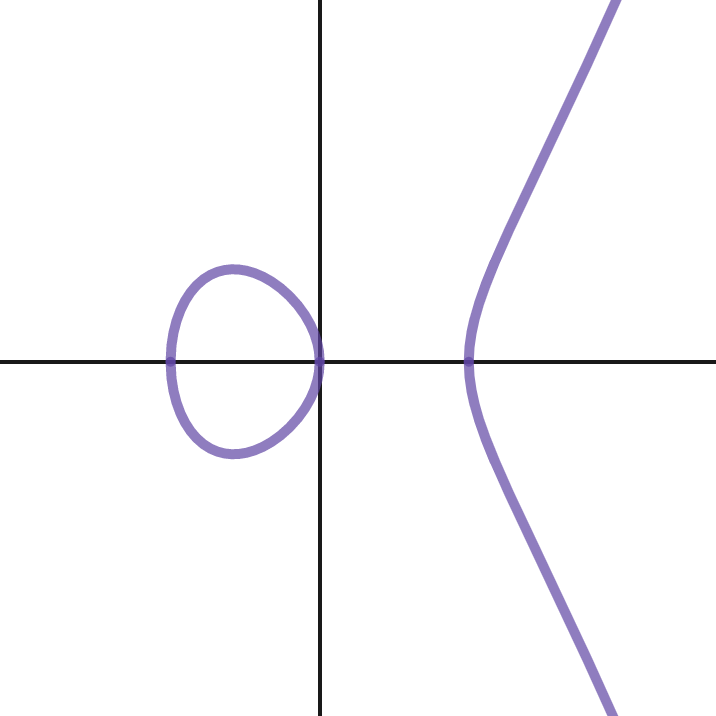
\includegraphics[width=0.5\textwidth]{9.png}
        \caption{$V(F)$ for $F:=w^2-z^3+z$. $V(F)$ is an elliptic curve! Plotted in \cite{Desmos}.}
        \label{fig:Fig9}
    \end{figure}
    We want to show $F$ is irreducible and $X$ is a nonsingular plane curve. Let's check that $X$ is nonsingular: $F_1=-3z^2+1$, $F_2=2w$ vanish at $\left(\pm\frac{1}{\sqrt{3}},0\right)$, but since these points aren't on the curve, we're good. So $F_1$, $F_2$ have no zeros in common. 
    
    Suppose that $F$ were reducible. There are no common factors that are functions of $z$, so the factors would have degree 1 in $w$. So it looks like $F=(w-g_1(z))(w-g_2(z))$. Since there is no middle term, $g_2=-g_1$ and $F$ factors as a difference of squares. But $z^3-z$ is not a square, since it has odd degree.
\end{example}
In general, if $F$ is irreducible, so is $V(F)$. The polynomial functions on $V(F)$ are basically $\cx[z,w]$, except that polynomials that differ by $F$ are identical. So in actuality, they are $\quotient{\cx[z,w]}{(F)}$, where $(F)$ is the ideal generated by $F$. Now, as $\cx[z,w]$ is a UFD and $F$ is irreducible, it is prime and so $\quotient{\cx[z,w]}{(F)}$ is an integral domain. However, if $F$ is \ita{reducible}, then $\quotient{\cx[z,w]}{(F)}$ is has zero divisors.

If $V(F)$ were disconnected, then indicator functions on the components are also zero divisors. This is partly why we required Riemann surfaces to be connected.
\begin{exercise}
    More generally, let $h(z)$ be a non-square polynomial. Show that $w^2-h(z)$ defines an irreducible plane curve that is nonsingular if and only if $h(z)$ has no repeated roots. $V(w^2-h(z))$ is called a hyperelliptic curve.
\end{exercise}
\begin{exercise}
    A \textbf{line} in $\cx^2$ is a curve defined by a degree 1 polynomial. A \textbf{conic} is defined by a polynomial of degree 2. Prove that a singular conic is the union of 2 lines.
\end{exercise}
\subsection{Topological Properties of Riemann Surfaces}
Say $X$ is a Riemann surface with two compatible charts $\phi_j:U_j\to V_j$ for $j\in\{1,2\}$, $U_1\cap U_2\neq\varnothing$. The charts must agree in orientation, else the transitions maps would not be conformal and hence not analytic. Hence any Riemann surface is an real orientable 2-manifold. If $X$ is a compact Riemann surface, it is a real orientable (smooth) manifold, and so is homeomorphic to a a genus $g$ surface. 
\subsection{Projective Plane Curves}
Define the \textbf{projective} plane $\p^2=\p_{\cx}^2$ to be the set 
\begin{equation}
    \p^2=\left(\cx^3\setminus\{(0,0,0)\}\right)\big/\sim
\end{equation}
where $(x_1,y_1,z_1)\sim(x_2,y_2,z_2)$ if $(x_1,y_1,z_1)=\lambda(x_2,y_2,z_2)$ for some $\lambda\in\cx^*$.

The equivalence class of $(x,y,z)$ is denoted by $[x,y,z]$. The $U_0:=\{[x,y,z]\mid x\neq0\}$ maps to $\cx^2$ as $[1,y,z]\mapsto(y,z)$ and similarly for $U_1$, $U_2$.
\section{February 12}
\subsection{Projective Plane Curves (cont'd)}
Recall that $\p^2$ is defined by 
\begin{equation}
    \p^2=\left(\cx^3\setminus\{(0,0,0)\}\right)\big/\sim
\end{equation}
where $[x,y,z]$ is the equivalence class of $(x,y,z)$. $\p^2$ is covered by 
\begin{equation}
    \begin{split}
        U_0&:=\{[1,y,z]\mid y,z\in\cx^*\}\\
        U_1&:=\{[x,1,z]\mid x,z\in\cx^*\}\\
        U_2&:=\{[x,y,1]\mid x,y\in\cx^*\}
    \end{split}
\end{equation}
The charts for each $U_j$ are 
\begin{equation}
    \begin{split}
        \varphi_0:[1,y,z]&\mapsto(y,z)\\
        \varphi_1:[x,1,z]&\mapsto(x,z)\\
        \varphi_2:[x,y,1]&\mapsto(x,y).
    \end{split}
\end{equation}
Let's confirm that these charts are indeed compatible. On $U_0\cap U_1$, 
\begin{equation}
    \begin{split}
        \tau_{0,1}&:(y,z)\mapsto[1,y,z]\\
        &=\left[\frac{1}{y},1,\frac{z}{y}\right]\\
        &\mapsto\left(\frac{1}{y},\frac{z}{y}\right),
    \end{split}
\end{equation}
which is analytic since $y\neq0$. A similar argument follows for the other transition maps.
\begin{remark}
    From now on, we will use the traditional $x$, $y$, and $z$ for our variables, and use subscript notation with these variables for partial derivatives. Note that $x$, $y$, and $z$ are all complex.
\end{remark}
$\p^2$ is compact, since (couldn't follow the argument here). 

If $F\in\cx[x,y,z]$ is a homogeneous polynomial, point evaluation at projective coordinates still doesn't make sense, but whether $F$ vanishes at $[x,y,z]$ is independent of the choice of homogeneous coordinates. The vanishing set $V(F)$ of a (squarefree) homogeneous polynomial is called a \textbf{projective plane curve}.

Now, let $X\in V(F)$ for some homogeneous $F\in\cx[x,y,z]$. Define $X_j:=X\cap U_j$ for $j\in\{0,1,2\}$. Then $X_2$ is the \underline{affine plane curve} $V(F(x,y,1))$. Similarly $X_0$ and $X_1$ are the affine plane curves of $F$ evaluated at $x=1$ and $y=1$, respectively. 

In a similar vein, for $f\in\cx[x,y]$ (not necessarily homogeneous), how do we form the \underline{projective closure} of $V(f(x,y))\in\cx^2$? By identifying $\cx$ with $U_2$ (henceforth we will canonically identify $U_2$ with $cx^2$), we can make $f$ a homogeneous polynomial in $x$, $y$, and $z$ by multiplying each term of $f$ with the appropriate factors of $z$ to make it homogeneous.
\begin{example}
    Recall the affine plane curve $V\left((y-x)(y-x-1)\right)$. The homogeneous polynomial according to the above construction is $(y-x)(y-x-z)$. So the closure of our affine curve is $V\left((y-x)(y-x-z)\right)\in\p^2$. Notice that the two components $V(y-x)$ and $V(y-x-z)$ meet where $z=y=0$, namely at $[1,1,0]$.
\end{example}
This illustrates a general phenomenon: any two curves in $\p^2$ intersect. Furthermore, if the curves have degrees $d$ and $e$, they meet in $d\cdot e$ points (with multiplicities counted appropriately). This is \textbf{B\'ezout's Theorem}. For example, if one of the curves has degree 1 (so linear) and intersects with a polynomial of degree $d$ at points outside of $U_2$, we can use the linear polynomial to make a substitution to get a degree $d$ polynomial in one variable.
\begin{definition}
    $X=V(F)$ is a \textbf{nonsingular plane curve} if at all points of $X$, at least one of $F_x$, $F_y$, or $F_z$ are nonzero.
\end{definition}
In fact, by Euler's identity, if $F$ has degree $d$, then 
\begin{equation}
    d\cdot F=xF_x+yF_y+zF_z.
\end{equation}
Thus if all three partials vanish, so does $F$. 
\begin{exercise}
    Prove Euler's identity. Also give an example for which $F$, $F_x$, and $F_y$ all vanish but $F_z$ does not.
\end{exercise}
\begin{exercise}
    Let $F$ be a homogeneous polynomial in $x$, $y$, $z$. Prove that a point $[x_0 , y_0 , z_0]$ with $z_0 \neq 0$, $\frac{\partial F}{\partial x} (x_0 , y_0 , z_0) \neq 0$ if and only if $\frac{\partial f}{\partial x} (x_0 , y_0) \neq 0$ where $f(x , y) = F(x, y, 1)$.
\end{exercise}
So $V(F)$ is a nonsingular projective plane curve if and only if each $V(F)\cap U_j$ is a nonsingular affine plane curve.

What is $\p^2\setminus U$? It's just
\begin{equation}
    \{[x,y,0]\mid x,y\text{ not both }0\}.
\end{equation}
This is a copy of $\p^1$. 

A nonsingular projective plane curve is a compact Riemann surface. Charts can all be taken to be of the form
\begin{equation}
    \frac{x}{y},\frac{x}{z},\frac{y}{x},\frac{y}{z},\frac{z}{x},\frac{y}{x}.
\end{equation}
\begin{exercise}
    Construct all nonsingular projective plane curves of all degrees $\geq1$.
\end{exercise}
\begin{example}
    Take our familiar elliptic curve $V(y^2-x^3+x)\subseteq\cx^2=U_2$. In $\p^2$, homogenize to get
    \begin{equation}
        y^2z-x^3+xz^2.
    \end{equation}
    Then 
    \begin{equation}
        \begin{split}
            F_x&=-3x^2+z^2\\
            F_y&=2yz\\
            F_z&=y^2+2xz.
        \end{split}
    \end{equation}
    We then show that $V(y^2z-x^3+xz^2)$ is nonsingular. Suppose there is a singular point on $V(y^2z-x^3+xz^2)$. Then $F_y=0$, so either $y=0$ or $z=0$. If $y=0$, then either $x=0$ or $z=0$ by $F_z$. If $x=0$, then by $F_x$, $z=0$, which is not allowed since $[0,0,0]$ does not exist in $\p^2$. If $z=0$, $F_x$ forces $x=0$ again. Thus this rules out $y=0$, and so $z=0$. This leads us back to the impossible points $[0,0,0]$ in all cases, and so no such singular point exists.
\end{example}
\section{February 17}
\subsection{Projective Plane Curves (cont'd)}
\begin{example}
    The elliptic curve $y^2-x^3+x$ is a nonsingular affine plane curve in $U_2=\cx^2$. Homogenize to get $y^2z-x^3+xz^2$ a nonsingular projective plane curve. $V(y^2z-x^3+xz^2)$ is the closure of $V(y^2-x^3+x)$ in $\p^2$.
    
    What if we multiplied by more powers of $z$? We get another connected component, $V(z^k)$. Outside of $U_2$ ($z=0$), we get another point on the curve: $[0,1,0]$. Let's find a chart for this point: in $U_1$, the curve becomes $g:=z-x^3+xz^2$.
    \begin{figure}[H]
        \centering
        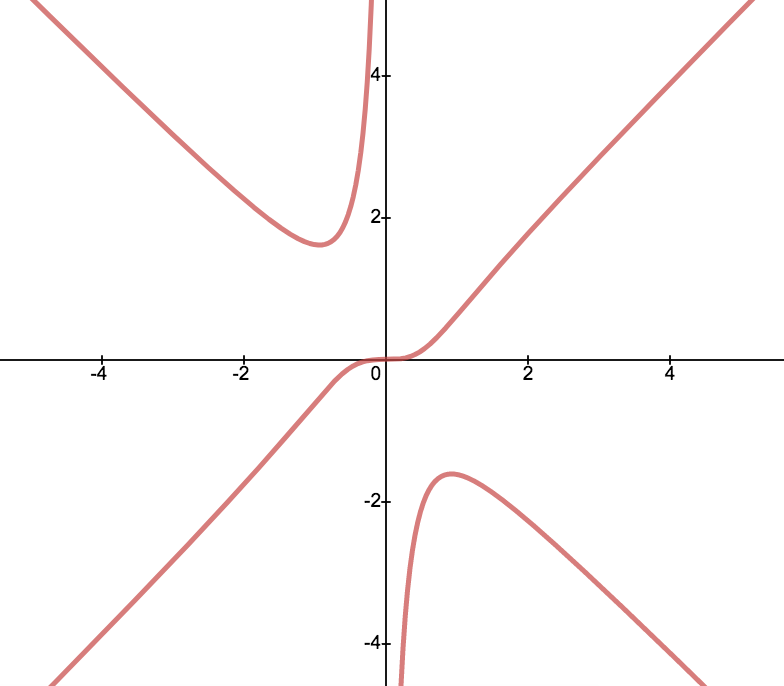
\includegraphics[width=0.5\textwidth]{10.png}
        \caption{$g$ plotted as a real polynomial of two variables. $g$ isn't anywhere near as nice as the elliptic curve. Plotted in \cite{Desmos}.}
        \label{fig:Fig10}
    \end{figure}
    At $(x,z)=(0,0)$,
    \begin{equation}
        \begin{split}
            g_x(0,0)&=\left.-3x^2+z^2\right|_{x=z=0}=0\\
            g_z(0,0)&=\left.1-2xz\right|_{x=z=0}=1.
        \end{split}
    \end{equation}
    Now, how do we define a parameter? We need to use either $\frac{x}{y}$ or $\frac{y}{z}$ (recall that evaluation of ratios of points in projective space are defined, not point evaluation). Since $g_x$ vanishes at $(x,z)=(0,0)$, pick $x$ to be the parameter, so our chart is taking $[x,y,z]\mapsto\frac{x}{y}$.
\end{example}
\begin{exercise}
    Show that the hyperelliptic curves $y^2-h(x)$ never compactify to nonsingular projective curves when $\deg h\geq4$.
\end{exercise}
\subsection{Functions on Riemann Surfaces}
\begin{definition}
    Let $X$ be a Riemann surface, $W\subseteq X$ an open set, $f:W\to\cx$. $f$ is called \textbf{holomorphic} at $p\in W$ if there exists a chart $(U,\varphi)$ with $p\in U$ such that $f\circ\inv{\varphi}:\varphi(U\cap W)\to\cx$ is analytic at $\varphi(p)$. $f$ is holomorphic on $W$ if it holomorphic at every $p\in W$.
\end{definition}
In a sense, $f$ is compatible with $\varphi$.
\begin{exercise}
    In the above situation, show that if $(V,\psi)$ is another chart with $p\in V$, then $f\circ\inv{\psi}:\psi(V\cap W)\to\cx$ is also analytic at $\psi(p)$.
\end{exercise}
\begin{example}
    \noindent
    \begin{itemize}
        \item For $X$ a Riemann surface, $W\subseteq X$ open and connected, $(W,\varphi)$ a chart, then $\varphi$ is holomorphic on $W$. Note that by construction, $W$ is itself a Riemann surface.
        \item Let $f$ be a function defined on a neighbhorhood of $\infty$ on the Riemann sphere. How do we tell whether $f$ is holomorphic at $\infty$? Take $w=\frac{1}{z}$, then write $f$ in terms of $w$, and see whether the singularity at $w=0$ is removable.
        \begin{itemize}
            \item $f(z)=z^2$ becomes $g(w)=\frac{1}{w^2}$, which has a pole of order 2 at $w=0$.
            \item The fractional linear map 
            \begin{equation}
                f(z)=\frac{z-1}{z+1}
            \end{equation}
            becomes 
            \begin{equation}
                g(w)=\frac{\frac{1}{w}-1}{\frac{1}{w}+1}=\frac{1-w}{1+w}
            \end{equation}
            for $w\neq0$, so $f$ has a removable singularity at $z=\infty$. Rewriting
            \begin{equation}
                f(z)=
                \begin{cases}
                    \frac{z-1}{z+1},&\quad z\in\cx\setminus\{-1\}\\
                    1,&\quad z=\infty
                \end{cases},
            \end{equation}
            then $f$ holomorphic at $\infty$. Here the Riemann surface is $\cx_{\infty}\setminus\{-1\}$. Note however that $f$ is still not defined on all of $\cx_{\infty}$, since it has a pole at $z=-1$. Eventually we will work with functions from $\cx_{\infty}\to\cx_{\infty}$, and so we don't have to worry about poles as much.
            \item In general, if $f$ is a rational function, say $f=\frac{g}{h}$ for $g,h\in\cx[z]$, $f$ is holomorphic at $\infty$ if and only if $\deg h\geq\deg g$.
        \end{itemize}
        \item On $\p^1$, if $f$ and $g$ are homogeneous of the same degree in $z$ and $w$, then $\frac{f}{g}$ is holomorphic wherever $g\neq0$.
        Surprisingly, all homogeneous polynomials in two complex variables factor completely!
        \item Each of the coordinate functions $x$ and $y$ on the nonsingular affine curve $X=V(F)$ is holomorphic. Indeed if $p\in X$ such that $x$ defines a chart near $p$, then $x$ is holomorphic there. If $x$ does not define a chart, then $y$ does since $F$ is nonsingular. Near $p$, $x=g(y)$ for some analytic $g$ thanks to the Implicit Function Theorem, so $x$ is still holomorphic.
        
        Similarly, if $X=V(F)$ is a nonsingular projective plane curve, then 
        \begin{equation}
            \underbrace{\frac{x}{z},\frac{y}{z}}_{U_2},\quad\underbrace{\frac{x}{y},\frac{z}{y}}_{U_1},\quad\underbrace{\frac{y}{x},\frac{z}{x}}_{U_0}
        \end{equation}
        are holomorphic wherever they are defined.
    \end{itemize}
\end{example}
\begin{exercise}
    Prove the Open Mapping Theorem for Riemann surfaces: let $X$ be a Riemann surface, $W\subseteq X$ open. If $f:W\to\cx$ is holomorphic, then $f(W)$ is open in $\cx$.
\end{exercise}
\begin{exercise}
    Prove the Maximum Principle for Riemann surfaces: let $X$ be a Riemann surface, $W\subseteq X$ open and \underline{connected}. If there exists $p\in W$ such that $|f(p)|\geq|f(w)|$ for all $w\in W$, then $f$ is constant on $W$.
\end{exercise}
Thus...
\begin{theorem}
    A holomorphic function on a compact Riemann surface is constant.
\end{theorem}
\section{February 19}
\subsection{Functions on Riemann Surfaces (cont'd)}
\begin{theorem}
    A holomorphic function on a compact Riemann surface is constant.
\end{theorem}
\begin{proof}
    Let $X$ be a compact Riemann surface, $f:X\to\cx$ holomorphic. Then $|f|:X\to\real$ is continuous, so its image is compact and thus there exists $p\in X$ such that $|f(p)|\geq|f(g)|$ for all $g\in X$. By Maximum Modulus Principle, $f$ is constant.
\end{proof}
\begin{exercise}
    Recall Liouville's Theorem, that a bounded entire function on $\cx$ is constant. Use the above theorem to prove this by showing that such a function extends to a holomorphic function on the Riemann sphere $\cx_{\infty}$.
\end{exercise}
\begin{definition}
    Miranda defines for a Riemann surface $X$ and for $W\subseteq X$ open,
    \begin{equation}
        \mathcal{O}_X(W):=\{f:W\to\cx\mid f\text{ is holomorphic }\}.
    \end{equation}
\end{definition}
$\mathcal{O}_X(W)$ is a $\cx$-algebra. For $V\subseteq W$, there is a restriction map
\begin{equation}
    \rho_{WV}:\mathcal{O}_X(W)\to\mathcal{O}_X(V).
\end{equation}
$\mathcal{O}_X$ is a \underline{contravariant functor}, mapping partially ordered set of open subsets of $X$ under inclusion to $\cx$-algebras.

Recall that $f$ is defined on an open subset of $\cx$ is \textbf{meromorphic} if its only singularities are removable or poles. Note that $f$ is meromorphic at $z_0\in\cx$ if and only if $f$ is the ratio of holomorphic functions with denominator not identically zero in a neighborhood of $z_0$.
\begin{definition}
    Let $X$ be a Riemann surface, $p\in X$, $f$ a function defined on a punctured neighborhood of $p$. $f$ has a \textbf{pole} at $p$ if there is a chart $(U,\varphi)$ with $p\in U$ such that $f\circ\inv{\varphi}$ has a pole at $\varphi(p)$. 
\end{definition}
If $U_1$ is another open set containing $p$ and $(U_1,\psi)$ is a chart, then we can write $f\circ\inv{\psi}=\underbrace{f\circ\inv{\varphi}}\circ\underbrace{\varphi\circ\inv{\psi}}$. So $f\circ\inv{\varphi}$ can be written as $\frac{g}{h}$ where $g$ and $h$ are holomorphic in some neighborhood of $\varphi(p)$. Thus
\begin{equation}
    f\circ\inv{\psi}=\frac{g\circ\varphi\circ\inv{\psi}}{h\circ\varphi\circ\inv{\psi}}.
\end{equation}
\begin{remark}
    This shows in general that the composition of a meromorphic function and a holomorphic function (in that order!) is meromorphic, but composing in the reverse order is \ita{not} necessarily meromorphic. For example, $f(z):=\frac{1}{z}$ is meromorphic and $g(z):=e^z$ is holomorphic, and $(f\circ g)(z)=\frac{1}{e^z}=e^{-z}$ is meromorphic (in fact holomorphic!), but $(g\circ f)(z)=e^{\frac{1}{z}}$ has an \underline{essential} singularity at $z=0$.
\end{remark}
\begin{definition}
    Let $X$ be a Riemann surface, $p\in X$, $f$ a function from a neighbhorhood of $p$ to $\cx$. $f$ is \textbf{meromorphic at $p$} if there is a chart $(U,\varphi)$, $p\in U$, such that $f \circ \inv{\varphi}$ is meromorphic at $\varphi(p)$.
\end{definition}
Similarly, we can define removable singularities and essential singularities on a Riemann surface.
\begin{example}
    \noindent
    \begin{itemize}
        \item A (homogeneous) rational function of degree $0$ on $\p^1$ is meromorphic.
        \item A rational function $\frac{g}{h}$ in $x$ and $y$ restricted to the connected nonsingular affine plane curve $V(F)$ is meromorphic provided $F\nmid h$.
        \item Similarly, a homogeneous degree $0$ rational function $\frac{g(x,y,z)}{h(x,y,z)}$ is meromorphic on the nonsingular projective plane curve $V(F)$ provided $F\nmid h$.
    \end{itemize}
\end{example}
\begin{definition}
    Miranda defines for a Riemann surface $X$ and all open $W\subseteq X$,
    \begin{equation}
        M_X(W):=\{f:W\to\cx\mid f\text{ is meromorphic on $W$ }\}.
    \end{equation}
\end{definition}
Note that $M_X(X)$ is a \underline{field}, but $M_X(W)$ is not always a field, unless $W$ is connected.
\begin{proposition}
    Let $X$ be a Riemann surface, $f$ a nonzero meromorphic function on $X$. The zeros and poles of $f$ are isolated.
\end{proposition}
\begin{proof}
    Let $p$ be a zero of $f$, $(U,\varphi)$ a chart with $p\in U$. Then $f\circ\inv{\varphi}$ is meromorphic on $\varphi(U)$, and so its zeros and poles are isolated. So $\varphi(p)$ has a neighborhood in which $f\circ\inv{\varphi}$ has no other zeros or poles.
\end{proof}
\begin{corollary}
    A meromorphic function on a \underline{compact} Riemann surface has finitely many zeros and finitely many poles.
\end{corollary}
\section{February 24}
\subsection{Multiplicity of Zeros and Poles}
Let $f , g \in \cx[x,y]$, and look at the intersections of $V(f)$ and $V(g)$ in $\cx^2$. [Missing this segue.] So the intersection points of the two curves are isolated. Then pass to $\p^2$ to see that there are only finitely many.

In general, the zeros and poles of a meromorphic function are isolated from \ita{any} points. For any $z_0$, a meromorphic has local form
\begin{equation}
    (z - z_0)^a g(z)
\end{equation}
for some $g$ analytic and nonzero at $z_0$. 

We'll now explore the question of \underline{multiplicity} of a zero or pole of a meromorphic function on a Riemann surface $X$. So let $X$ be a Riemann surface, $W \subseteq X$ open for which $f$ is meromorphic, $p \in W$.Take some chart $(U , \varphi)$ where $p \in U \subseteq W$; let $z_0 := \varphi(p)$. Then in a neighborhood of $z_0$, $f \circ \inv{\varphi}$ has Laurent expansion 
\begin{equation}
    \sum\limits_{n = -\infty}^{\infty} a_n (z - z_0)^n.
\end{equation}
There exists 
\begin{equation}
    \min \setb{n \mid a_n \neq 0} =: n_0.
\end{equation}
Now suppose that $(U_1 , \varphi_1)$ with $p \in U_1 \subseteq W$ is another chart. Use $w$ for the complex coordinate in $\varphi_1(U_1)$, and let $w_0 := \varphi_1(p)$. Let $T = \varphi \circ \inv{\varphi_1}$ expressing $z$ locally in terms of $w$; now, $T$ has an analytic inverse $\inv{T}$; note that $w = \left( \inv{T} \circ T \right)(w)$ for all $w$ in this neighborhood. Taking derivatives of both sides gives 
\begin{equation}
    1 = \left( \inv{T} \right)'(w) T(w) \underbrace{T'(w)}_{\neq 0}.
\end{equation}
So in a neighborhood of $w_0$, 
\begin{equation}
    T(w) = z_0 + \underbrace{c_1}_{= T'(w) \neq 0} (w - w_0) + O \left( |w - w_0|^2 \right).
\end{equation}
So $T(w) - z_0 = c_1(w - w_0)g(w)$, where $g$ is analytic at $w_0$ and $g(w_0) = 1$. To calculate the Laurent series for $f \circ \inv{\varphi_1}$, first note that 
\begin{equation}
    T(w) = w_0 + c_1 (w - w_0) g(w).
\end{equation}
Every power of $g$ expands as 1 to higher order terms. So the lowest power term is 
\begin{equation}
    a_{n_0} \big( c_1 (w - w_0) g(w) \big)^{n_0},
\end{equation}
which looks like 
\begin{equation}
    a_{n_0} c_1^{n_0} (w - w_0)^{n_0} (1 + \dotsb).
\end{equation}
This $n_0$ is called the \textbf{order} of $f$ at $p$; we just showed that it's well-defined!
\begin{exercise}
    For meromorphic functions $f$, $g$ at a point $p$ on a Riemann surface $X$, prove the following:
    \begin{align*}
        \ord_p (f g) & = \ord_p (f) + \ord_p (g), \\
        \ord_p \left( \frac{f}{g} \right) & = \ord_p (f) - \ord_p (g), \\
        \ord_p (f + g) & \geq \min \{ \ord_p (f) , \ord_p (g) \}.
    \end{align*}
    For the third one, give examples of equality and strict inequality.
\end{exercise}
\begin{example}
    \noindent
    \begin{itemize}
        \item Let $f , g \in \cx[z]$. Then $\frac{f}{g}$ is a rational function. Let $m := \deg f$, $n := \deg g$. Let's calculate $\ord_p \left( \frac{f}{g} \right)$. Write 
        \begin{align}
            f(z) & = a_m z^m + \dotsb, && g(z) = b_n z^n + \dotsb.
        \end{align}
        Then 
        \begin{equation}
            \frac{f(z)}{g(z)} = \frac{z^{-m} \left( a_m + a_{m-1}z + \dotsb \right)}{z^{-n} \left( b_n + b_{n-1}z + \dotsb \right)} = z^{n - m} h(z)
        \end{equation}
        where $h$ is a nonzero rational function that is defined and does not vanish at zero. Note that these are counting $z$ with multiplicity, so suppose that there are $m$ zeros and $n$ poles. So, 
        \begin{equation}
            \sum\limits_{p \in \cx} \ord_p \left( \frac{f}{g} \right) = m - n + n - m = 0.
        \end{equation}
        \item Let $L \subset \cx$ be a lattice, $X := \cx / L$. Then only functions on $X$ are constant. What about \underline{meromorphic} functions? Note that if $f$ is meromorphic on $X$, composing $f$ with the covering map $\cx \to X$ gives a meromorphic function $F$ on $\cx$. $F$ has the property that $F(z+w) = f(z)$ for all $z \in \cx$ (where $F$ is defined), $w \in L$. Such a function is called \textbf{double periodic} or \textbf{elliptic} with period lattice $L$. Conversely, given such a doubly periodic $F$ with period lattice $L$, this gives a well-defined meromorphic function $f$ on $X$ given by $f(p) = F$ evaluated at any preimage of $p$ under the covering map. So there is a nice one-to-one correspondence
        \begin{equation}
            \setb{ \text{$f$ meromorphic on $X$} } \xlongleftrightarrow{} \left\{ \parbox{15em}{$F$ meormorphic on $\cx$, \\ doubly periodic with lattice $L$} \right\}.
        \end{equation}
        An example of such a function is the Weierstrass $\zeta$-function:
        \begin{equation}
            \zeta(z) = \frac{1}{z^2} + \sum\limits_{
            \substack{
                w \in L \\
                w \neq 0
                }
            }
            \left( \frac{1}{(z-w)^2} - \frac{1}{w^2} \right).
        \end{equation}
    \end{itemize}
\end{example}
\subsection{Harmonic Functions on a Riemann Surface}
``Recall'' that $h : \real^2 \to \real$ is \textbf{harmonic} on some domain $U$ if $h_{xx} + h_{yy} = 0$ on $U$. A complex-valued function is harmonic if and only if its real and imaginary parts are harmonic.
\begin{remark}
    Note that a holomorphic function is harmonic; this follows from the Cauchy-Riemann equations. However, this implication does \ita{not} reverse; consider the conjugate map $x + iy \mapsto x - iy$.
\end{remark}
We transport harmonicity to a Riemann surface $X$ via charts in the usual way. Suppose $f$ is twice continuously differentiable at $p \in X$. Then $f$ is \textbf{harmonic} at $p$ if there is a chart $(\varphi , U)$ with $p \in U$ such that $f \circ \inv{\varphi}$ is harmonic in a neighborhood of $\varphi(p)$. This is independent of the choice of chart; the proof is given in Miranda.
\begin{exercise}
    If $h$ is harmonic and $T$ is holomorphic, prove that $h \circ T$ is harmonic (use Cauchy-Riemann equations).
\end{exercise}
\section{February 26}
\subsection{Classifying Meromorphic Functions on \texorpdfstring{$\cx_{\infty}$}{Coo}}
\begin{lemma}
    Let $f$ be an entire function with a pole at $\infty$. Then $f$ is a polynomial.
\end{lemma}
\begin{proof}
    Write $f$ as 
    \begin{equation}
        f(z) = \sum\limits_{n = 0}^{\infty} a_n z^n,
    \end{equation}
    which converges on all of $\cx$. As a Laurent series at $\infty$ in terms of $w = \frac{1}{z}$, we get 
    \begin{equation}
        \sum\limits_{n = 0}^{\infty} a_n w^{-n} = \sum\limits_{n = -\infty}^{0} a_{-n} w^n.
    \end{equation}
    Since $f$ has a pole, there exists $n_0 = \max \setb{n \mid a_n \neq 0}$. Thus, $f$ is a polynomial.
\end{proof}
\begin{proposition}
    Let $f$ be a meromorphic function on $\cx_{\infty}$. Then $f$ is a rational function.
\end{proposition}
\begin{proof}
    If $f$ has a pole at $\infty$, then $\frac{1}{f}$ does not. So it suffices to consider the case in which $f$ does not have a pole at $\infty$. Since $\cx_{\infty}$ is compact, $f$ has finitely many poles, say $p_1 , \dotsc, p_k$ with multiplicities $n_1 , \dotsc, n_k$, respectively. Then 
    \begin{equation}
        g(z) = (z - p_1)^{n_1} \dotsm (z - p_k)^{n_k} f(z)
    \end{equation}
    is entire. In a neighborhood of $\infty$, $g$ is 
    \begin{equation}
        \left( \frac{1}{w} - p_1 \right)^{n_1} \dotsm \left( \frac{1}{w} - p_k \right)^{n_k} f.
    \end{equation}
    So $w^{n_1 + \dotsb + n_k} g$ is analytic at $\infty$, and so $g$ has at worst a pole of order $n_1 + \dotsb + n_k$ at $\infty$. By the Lemma, $g$ is a polynomial. So
    \begin{equation}
        f(z) = \frac{g(z)}{(z - p_1)^{n_1} \dotsm (z - p_k)^{n_k}}
    \end{equation}
    is rational.
\end{proof}
\subsection{Meromorphic Functions on a Torus}
As before, let $L = \z \omega_1 + \z \omega_2$ be a lattice in $\cx$, $X = \cx / L$. Let $f$ be a meromorphic function on $X$, $F$ its corresponding periodic meromorphic function on $\cx$.
\begin{figure}[H]
    \centering
    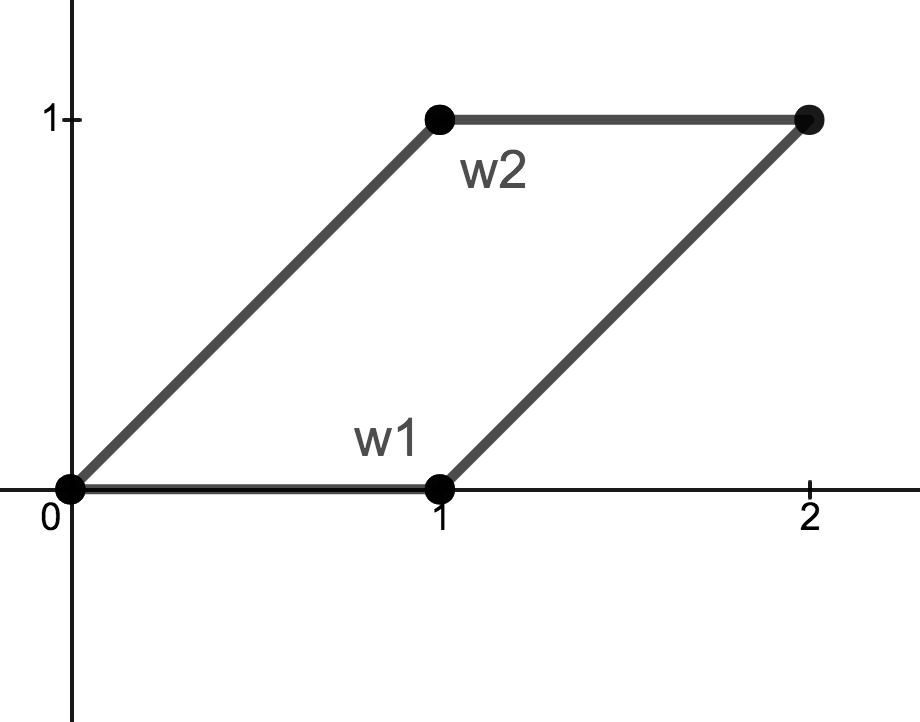
\includegraphics[width = 0.5\textwidth]{11.png}
    \caption{Fundamental domain for the torus $\cx / L$. Plotted in \cite{Desmos}.}
    \label{fig:Fig11}
\end{figure}
Choose $P$ to be a parallelogram giving a fundamental domain for $F$, such that none of the zeros or the poles of $F$ lie on the boundary $\partial B$ of $P$. Let $\gamma$ be an oriented boundary curve of $P$, given by
\begin{equation}
    \begin{split}
        \gamma_1(t) & := z_0 + \omega_1 t \\
        \gamma_2(t) & := z_0 + \omega_1 + \omega_2 t \\
        \gamma_3(t) & := z_0 + \omega_2 + \omega_1 t \\ 
        \gamma_4(t) & := z_0 + \omega_2 t.
    \end{split}
\end{equation}
where $t \in [0,1]$. Then we can stitch these together, \ita{i.e.} concatenation of paths (as in algebraic topology!) to form the oriented boundary $\partial P$:
\begin{equation}
    \gamma := \gamma_1 \ast \gamma_2 \ast -\gamma_3 \ast -\gamma_4.
\end{equation}
The negatives are necessary since we defined $\gamma_3$ and $\gamma_4$ to go outward and right, as in the typical diagrams drawn to demonstrate vector addition with arrows. Then 
\begin{equation}
    \frac{1}{2 \pi i} \int_{\gamma} 
    F = \frac{1}{2 \pi i} \left( \int_{\gamma_1} F + \int_{\gamma_2} F - \int_{\gamma_3} F - \int_{\gamma_4} F \right).
\end{equation}
Then 
\begin{equation}
    \begin{split}
        \int_{\gamma_1} F \,\mathrm{d}z & = \int_0^1 F(z_0 + t \omega_1) \omega_1 \, \mathrm{d}t \\
        \int_{\gamma_1} F \,\mathrm{d}z & = \int_0^1 \underbrace{ F(z_0 + t \omega_1 + \omega_2) }_{ = F(z_0 + t \omega_1)} \omega_1 \, \mathrm{d}t
    \end{split}
\end{equation}
since $F$ is double periodic. Thus $\int_{2 \pi i} \int_{\gamma} F = 0$, and therefore the sum of the residues of these poles of $F$ is 0.
\begin{corollary}
    Let $L$ be a lattice in $\cx$, $X = \cx / L$, $f$ meromorphic on $X$. Then $f$ cannot have a single simple pole.
\end{corollary}
\noindent \underline{Recall}: If $\gamma$ is a simple closed curve, $f$ meromorphic, $\gamma$ a smooth closed curve not passing through any of the poles or zeros of $f$, then 
\begin{equation}
    \frac{1}{2 \pi i} \int_{\gamma} \frac{f'(z)}{f(z)} \, \mathrm{d}z = \sum\limits_{p \in X} \ord_p(f),
\end{equation}
where the sum over $p \in X$ is for all $p$ enclosed by $\gamma$. 
\begin{exercise}
    Use integration to show that for $L$ a lattice, $X = \cx / L$, $f$ meromorphic on $X$,
    \begin{equation}
        \sum\limits_{p \in X} \mathrm{ord}_p (f) = 0.
    \end{equation}
\end{exercise}
Recall that our $X = \cx / L$ has the structure of a group. How many elements of order $n$ does $X$ have?
\begin{figure}[H]
    \centering
    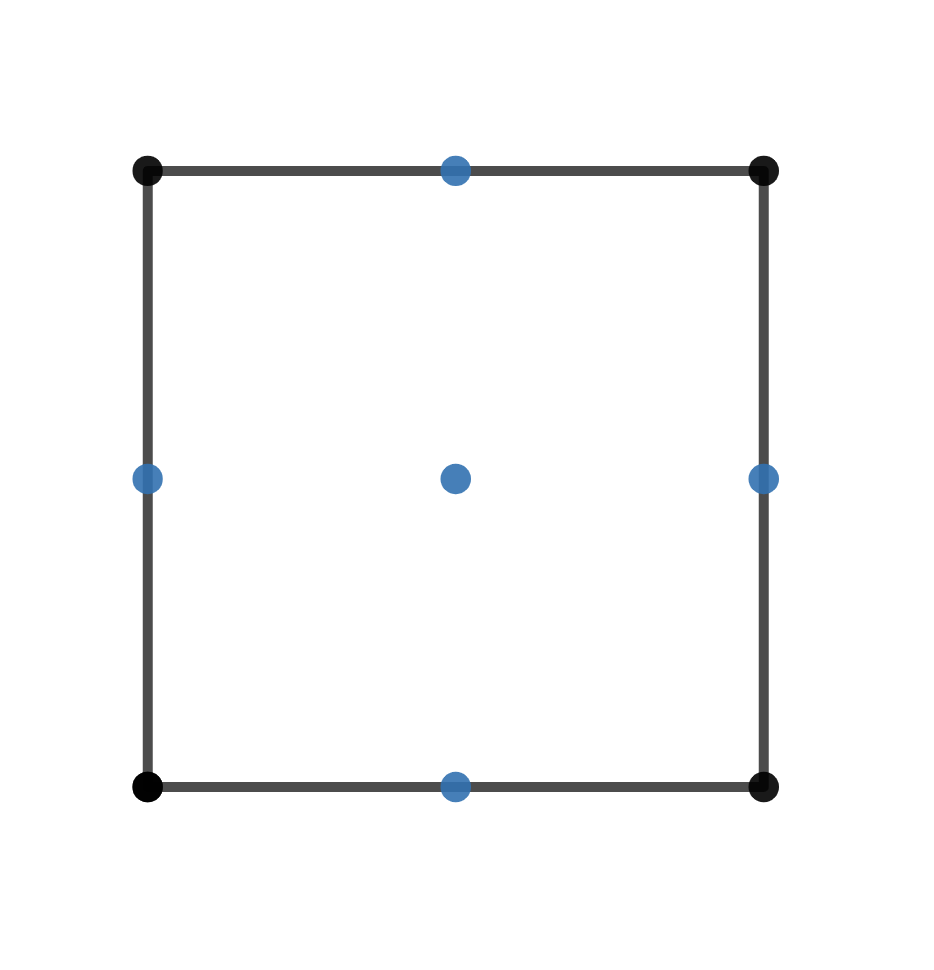
\includegraphics[width = 0.5\textwidth]{12.png}
    \caption{For example, take $L$ to be the integer lattice (so $L = \z[i]$). Then $\cx / L$ has 5 elements of order two, labeled in blue. Plotted in \cite{Desmos}.}
    \label{fig:Fig12}
\end{figure}
In general, $X$ has $n^2 - 1$ elements of order $n$. 

This time, we'll evaluate 
\begin{equation}
    \frac{1}{2 \pi i} \int_{\gamma} \frac{z F'(z)}{F(z)} \, \mathrm{d}z,
\end{equation}
where $F$ is the doubly periodic meromorphic function on $\cx$ corresponding to a meromorphic function on $X$ and $\gamma$ is the boundary curve of a fundamental parallelogram $P$, again chosen so that it contains no zeros or poles of $F$. Recall from Exercise 10 that this gives the sum $\ord_p(f) p$ where $p$ runs over all zeros and poles of $F$ contained inside of $P$. Let $\gamma_1$, $\gamma_2$, $\gamma_3$, $\gamma_4$ as above, and stay tuned for next time to find out what we do next!
\section{March 2}
\subsection{Meromorphic Functions on a Torus (cont'd)}
Let $L$ be a lattice in $\cx$, say $L = \z \omega_1 +  \z \omega_2$ where $\omega_1 , \omega_2 \in \cx$ are linearly independent over $\real$. Let $X = \cx / L$, $f$ meromorphic on $X$ with zeros $\setb{q_j}_{j=1}^r$ and poles $\setb{p_j}_{j=1}^r$.

Choose a fundamental parallelogram $P$ whose boundary does not contain any zeros or poles of $f$. Let $\gamma$ be the oriented boundary of $P$. Then 
\begin{equation}
    \frac{1}{2\pi i}\int_{\gamma} z \frac{f'(z)}{f(z)} \,\mathrm{d}z = \sum\limits_{p \in X} p \cdot \ord_p(f).
\end{equation}
Then 
\begin{equation}
    \begin{split}
        \int_{\gamma_1} z \frac{f'(z)}{f(z)} \,\mathrm{d} z & = \int_0^1 \frac{(z_0 + t \omega_1) f'(z_0 + t \omega_1)}{f(z_0 + t \omega_1)} \\ 
        \int_{\gamma_3} z \frac{f'(z)}{f(z)} \,\mathrm{d} z & = \int_0^1 \frac{(z_0 + \omega_2 + t \omega_1)f'(z_0 + \omega_2 + t \omega_1)}{f(z_0 + \omega_2 + t \omega_1)} \omega_1 \,\mathrm{d}t \\
        & = \int_0^1 \frac{(z_0 + \omega_2 + t \omega_1)f'(z_0 + t \omega_1)}{f(z_0 + \omega_2 + t \omega_1)} \omega_1 \, \mathrm{d}t
    \end{split}
\end{equation}
where the last equality is due to $f$ being doubly periodic, and so its derivative $f'$ also is. Then 
\begin{equation}
    \begin{split}
        \int_{\gamma_1} z \frac{f'(z)}{f(z)} \, \mathrm{d} z - \int_{\gamma_3} z \frac{f'(z)}{f(z)} \,\mathrm{d} z & = -\omega_2 \int_{\gamma_1} z \frac{f'(z)}{f(z)} \,\mathrm{d} z \\
        & = -\omega_2 \int_0^1 \frac{f'(z_0 + t \omega_1)}{f(z_0 + t \omega_1)} \omega_1 \,\mathrm{d} t \\
        & = -\omega_2 \int_{f \circ \gamma_1} \frac{\mathrm{d} z}{z},
    \end{split}
\end{equation}
where the last equality is due to $f \circ \gamma_1$ being a closed curve by periodicity of $f$ (note that $\gamma_1$ is itself \ita{not} a closed curve, but that its endpoints are identified together by periodicity of $f$). So 
\begin{equation}
    \int_{\gamma_1} z \frac{f'(z)}{f(z)} \,\mathrm{d} z - \int_{\gamma_3} z \frac{f'(z)}{f(z)} \,\mathrm{d} z = -\omega_2 2\pi i \underbrace{n(f \circ \gamma_1 ; 0)}_{\text{winding number}},
\end{equation}
and so the difference of the integrals is (apart from a factor of $2 \pi i$) an integer multiple of $\omega_2$. Similarly,
\begin{equation}
    \frac{1}{2 \pi i} \left[ \int_{\gamma_2} z \frac{f'(z)}{f(z)} \,\mathrm{d} z - \int_{\gamma_4} z \frac{f'(z)}{f(z)} \,\mathrm{d} z \right]
\end{equation}
is an integer multiple of $\omega_2$. Thus 
\begin{equation}
    \int_{\gamma} z \frac{f'(z)}{f(z)} \,\mathrm{d} z = m \omega_1 + n \omega_2
\end{equation}
for some $m , n \in \z$. So on $X$, 
\begin{equation}
    \sum\limits_{p \in X} p \cdot \ord_p (f) = 0
\end{equation}
in the group law of $\cx / L$.
\subsection{Morphisms of Riemann Surfaces}
What should it mean for a map $f : X \to Y$ of Riemann surfaces to be \underline{holomorphic} at a point $p \in X$?

Choose a chart $(U , \varphi)$ on $X$ such that $p \in U$ and a chart $(V , \psi)$ on $Y$ such that $\varphi(p) \in V$. Then we would like $\psi \circ f \circ \inv{\varphi}$ (figure out the domain for that!) to be holomorphic at $\varphi(p)$. For further charts $(U_1 , \varphi_1)$, $(V_1 , \psi_1)$, \begin{equation}
    \psi_1 \circ f \circ \inv{\varphi_1} = \big( \underbrace{\psi_1 \circ \inv{\psi}}_{\text{holomorphic}} \big) \circ \big( \underbrace{\psi \circ f \circ \inv{\varphi}}_{\text{holomorphic}} \big) \circ \big( \underbrace{\varphi \circ \inv{\varphi_1}}_{\text{holomorphic}} \big).
\end{equation}
\begin{example}
    Let $f$ be a meromorphic function on the Riemann surface $X$. We claim that $f$ gives rise to a holomorphic map $X \to \cx_{\infty}$, by sending the poles to $\infty$. 
    Consider a chart around some pole $p$ of $f$ and the usual chart $w = \frac{1}{z}$ around $\infty$. So assigning the point $w = 0$ (\ita{i.e.}, $\infty$) to $p$ defines a holomorphic map near $p$.
    On the other hand, a holomorphic map $X \to \cx_{\infty}$ gives a meromorphic function $X \to \cx$. So there is (almost) a one-to-one correspondence
    \begin{equation}
        \setb{ \text{ meromorphic functions on $X$ } } \xlongleftrightarrow{} \setb{ \text{ holomorphic maps $X \to \cx_{\infty}$ } }.
    \end{equation}
    This correspondence isn't quite perfect, since the holomorphic function $X \to \cx_{\infty}$ given by $f \equiv \infty$ is not meromorphic on $X$.
\end{example}
\begin{exercise}
    Let $X$, $Y$, $Z$ be Riemann surfaces, $f : X \to Y$, $g: Y \to Z$ holomorphic. Show that $g \circ f$ is holomorphic.
\end{exercise}
\noindent \underline{Recall}: For a Riemann surface $X$, define $\mathcal{O}_X(W)$ for all open $W \subseteq X$ as the collection of all holomorphic functions on $W$. If $f : X \to Y$ is a holomorphic map of Riemann surfaces and $V \subseteq Y$ is an open set, then any holomorphic map $g$ on $V$ gives rise to $g \circ f : \inv{f}(V) \to \cx$ holomorphic. Then we get $f^* : \mathcal{O}_Y(V) \to \mathcal{O}_X \left( \inv{f}(V) \right)$.
\begin{definition}
    An \textbf{isomorphism} of Riemann surfaces is a morphism with an inverse.
\end{definition}
\begin{theorem}
    A nonconstant holomorphic map $f : X \to Y$ of Riemann surfaces is \underline{open}.
\end{theorem}
\begin{corollary}
    A \underline{monomorphism} (injective holomorphic map) $f : X \to Y$ of Riemann surfaces is an isomorphism onto its image.
\end{corollary}
Recall that a compact subspace of a Hausdorff space is closed. Now, let $X$ be a compact Riemann surface, $Y$ any Riemann surface, $f : X \to Y$ holomorphic and nonconstant. Then $f(X)$ is open and compact in $Y$, and hence closed. Since $Y$ is connected, $f(X) = Y$, so $f$ is onto and $Y$ is compact.
\begin{exercise}
    Show that $\p \cong \cx_{\infty}$ via 
    \begin{equation}
        [z , w] \mapsto \left( \frac{2 \mathrm{Re}( z \overline{w} )}{|z|^2 + |w|^2} , \frac{2 \mathrm{Im}( z \overline{w} )}{|z|^2 + |w|^2} , \frac{|z|^2 - |w|^2}{|z|^2 + |w|^2} \right).
    \end{equation}
    Show that this map is well-defined and that the codomain is correct.
\end{exercise}
\section{March 4}
\subsection{Local Normal Form}
\begin{proposition}
    Let $f , g : X \to Y$ be holomorphic maps of Riemann surfaces. If $f = g$ on a set with an accumulation point, then $f = g$.
\end{proposition}
\begin{proof}
    Let 
    \begin{equation}
        S := \setb{ x \in X \mid f(x) = g(x) },
    \end{equation}
    and let $x_0$ be an accumulation point of $S$. Let $(U , \varphi)$ be a chart on $X$ with $x_0 \in U$, and let $(V , \psi)$ be a chart on $Y$ with $f(x_0) \in V$. Choose $U$ so that $f(U) \subseteq V$ (we can always do this by restricting to the subset of $U$ that gets mapped to $V$ under $f$). Then $\psi \circ f \circ \inv{\varphi} : \varphi(U) \to \cx$ is analytic and is equal to $\psi \circ g \circ \inv{\varphi} : \varphi(U) \to \cx$ on some subset of $\varphi(S \cap U)$, with an accumulation point. By Complex Analysis, $\psi \circ f \circ \inv{\varphi} = \psi \circ g \circ \inv{\varphi}$ on $\varphi(U)$, so $f = g$ on $U$. Let 
    \begin{equation}
        T := \setb{x \in X \mid f(p) = g(p) \text{ for all $p$ in some neighborhood of $x$}}.
    \end{equation}
    $T$ is open: if $x \in T$, $f = g$ on some neighborhood $N$ of $x$, and as $N$ is a neighbhorhood of each of its points, $N \subseteq T$. As $x_0 \in T$, $T \neq \varnothing$. To show that $T$ is closed, let $x_1$ be an accumulation point of $T$, and choose a neighborhood $M$ of $x_1$. Then $f$ and $g$ agree on $M \cap T$, which has an accumulation point. So $f = g$ on $M$ and $x_1 \in T$. So $T \subseteq X$ is a nontrivial clopen set of a connected space, and thus $T = X$.
\end{proof}
Now let $f : X \to Y$ be a holomorphic function of Riemann surfaces, $y \in Y$. What does $\inv{f} \left( \setb{y} \right)$ look like? If $f$ is constant, then there's not much to say; so suppose $f$ is constant. Then $\inv{f} \left( \setb{y} \right)$ is discrete! So if $X$ is compact, $\inv{f} \left( \setb{y} \right)$ is \underline{finite}.

OK, let's recap: $A \subseteq X$ is \underline{discrete} if the subspace topology on $A$ inherited from $X$ is the discrete topology. Now here's the lemma we needed:
\begin{lemma}
    A closed discrete subspace of a compact space is finite.
\end{lemma}
Now, fix a nonconstant holomorphic $f : X \to Y$, $X$ compact. Then $Y$ is compact. Let $x \in X$, $(U , \varphi)$ a chart on $X$ such that $x \in U$. Let $y := f(x)$, and take a chart $(V , \psi)$ on $Y$ such that $y \in Y$, and suppose that $f(U) \subseteq V$. Take \begin{equation}
    \underbrace{\psi \circ f \circ \inv{\varphi}}_{=: T} : \underbrace{\varphi(U)}_{z} \to \underbrace{\cx}_{w}.
\end{equation}
Choose $\varphi, \psi$ centered at $x,y$, respectively. Then $T(0) = 0$, so locally $T(z)$ looks like $w = z^r g(z)$ for some $r \in \z^+$ and $g$ analytic and nonzero at $z = 0$. Then there is some branch of the logarithm (just write it as $\log$) such that $\log \circ g$ is analytic in a neighborhood of $z = 0$. Then there exists $R$ analytic such that 
\begin{equation}
    \big( R(z) \big)^r = g(z)
\end{equation}
(so $R(z) = e^{\frac{1}{r} \log \big( g(z) \big)}$) on a neighborhood of $z = 0$. Furthermore, $R(0) \neq 0$, since $g(0) \neq 0$. So 
\begin{equation}
    w = \big( \underbrace{z R(z)}_{=:k(z)} \big)^r.
\end{equation}
Note that $\varphi_1 = k \circ \varphi$ is a chart on some neighborhood of $x$, since $k'(0) \neq 0$, so locally $k$ is injective. So in a neighborhood of $0$,
\begin{equation}
    \begin{split}
        \left( \psi \circ f \circ \inv{\varphi_1} \right)(z) & = \left( \psi \circ f \circ \inv{\varphi} \circ \inv{k} \right)(z) \\
        & = \Big( k \left( \inv{k}(z) \right) \Big)^r \\
        & = z^r.
    \end{split}
\end{equation}
Locally, every such $f$ has charts $(U , \varphi)$ on $X$, $(V , \psi)$ on $Y$ with $x \in U$ such that $\left( \psi \circ f \circ \inv{\varphi} \right)(z) = z^r$ for all $z \in \varphi(U)$. This is called \textbf{Local Normal Form}.

What about for points near $x$ in $U$? For $q \in f(U) \setminus \setb{ f(x) }$, $q$ has $r$ distinct preimages in $U$. What is the $r$ value for such a $q$? This corresponds under $\psi$ to a point near $0$, say $\tilde{w}$ and a preimage $\tilde{z}$ of $\tilde{w}$, so $\tilde{w} = \left( \tilde{z} \right)^r$, now in powers of $z - \tilde{z}$, $T$ looks like 
\begin{equation}
    \tilde{w} + \underbrace{ T'(\tilde{z}) }_{\neq 0}(z - \tilde{z}) + \dotsb
\end{equation}
so the first power is present, and so the $r$ value is 1.
\newline
\newline
\underline{Upshot}: The set
\begin{equation}
    \setb{x \in X \mid \text{local normal form of $f$ has $r$ value $>1$}}
\end{equation}
is \underline{discrete}. This $r$ is called the \textbf{valency} of $f$ or the \textbf{ramification index} of $f$ at $x$; if this index $r > 1$, $x$ is called a \textbf{ramification point} and $f(x)$ is called a \textbf{branch point}.
\section{March 9}
\subsection{From Last Time}
Let $f : X \to Y$ be a nonconstant map of Riemann surfaces. Then $f$ has a \underline{local normal form} $z \mapsto z^r$, where the $r$-value is called the \underline{valency} (also ``ramification index''). $x$ is called a \underline{ramification point} and $f(x)$ a \underline{branch point}.
\begin{example}
    Let $X = V(f) \subseteq \cx^2$, where $f := y^2 - x^3 + x \in \cx[x,y]$ is our favorite elliptic curve. Note that $V(f)$ is not compact, but its projective closure is.Take $\pi : (x,y) \mapsto x$. What is the valency of $\pi$ at $(0,0)$?
    
    First, let's find a chart: $f_y(0,0) = 0$ but $f_x(0,0) = 1 \neq 0$, so $x = g(y)$ in a neighborhood of $(0,0)$ for $g$ holomorphic. Then 
    \begin{equation}
        y^2 = x^3 - x = x(x^2 - 1),
    \end{equation}
    where $x^2 - 1$ is nonzero at $(0,0)$, and so has a square root $R(y)$ locally that is nonvanishing. Hence 
    \begin{equation}
        x = \left[ \frac{y}{R(y)} \right]^2,
    \end{equation}
    so the valency is 2.
\end{example}
\begin{exercise}
    Let $f$ be a polynomial in 2 variables, defining the Riemann surface $X = V(f)$ with $f_y$ not $\equiv 0$. Prove that $p \in X$ is a ramification point for $\pi$ if and only if $f_y(p) = 0$.
\end{exercise}
\begin{exercise}
    Find an example of such an $f$ with a branch point having both a ramified and unramified preimage under $\pi$.
\end{exercise}
\begin{exercise}
    Find the other ramification points of $\pi : X \to \cx$ and their valencies, where $X = V(y^2 - x^3 + x)$, and $\pi : X \to \cx$, $\pi : (x,y) \mapsto x$.
\end{exercise}
\begin{example}
    To continue the above example, look at the projective closure $\overline{X} \subseteq \p^2$ (so $\overline{X} = V(y^2z - x^3 + xz^2)$. Does $\pi$ extend to a map on all of $\overline{X}$? Well, gee (courtesy of \cite{Valentini}). Our $\pi$, at least on $U_2$ ($=\cx^2$) is of the form $[x,y,z] \mapsto \frac{x}{z}$. This gives us a meromorphic function $\overline{\pi}$ on $X$, \ita{i.e.}, a holomorphic function from $\overline{X}$ to $\p^1 \cong \cx_{\infty}$, $\overline{\pi} : [x,y,z] \mapsto [x,y]$. The part of $\overline{X}$ not in $X$ is where $z = 0$ (these are where the so called ``infinite points'' of $V(f)$ reside). Set $z = 0$; this gives us $x = 0$ and $y = 1$. So our infinite point is $[0,1,0]$. What is the valency of $\overline{\pi}$ at this point? We can't just plug in $[0,1,0]$, this spits out $[0,0]$. So we dehomogenize at $U_1$, where the local equation in the $xz$-plane is 
    \begin{equation}
        z - x^3 + xz^2.
    \end{equation}
    At $(0,0)$, $f_x$ vanishes so use $x$ as the chart. Then $z = x^3 - xz^2$, so 
    \begin{equation}
        \begin{split}
            z + xz^2 & = x^3 \\
            z (\underbrace{1 + xz}_{\text{nonvanishing}}) & = x^3.
        \end{split}
    \end{equation}
    So $1 + xz$ has a nonvanshing local cube root $R(x)$, so 
    \begin{equation}
        z = \left[ \frac{x}{R(x)} \right]^3.
    \end{equation}
    The original map $\overline{\pi}$ mapped to $\frac{x}{z}$, so 
    \begin{equation}
        \frac{x}{z} = \frac{R(x)^3 x}{x^3} = R(x)^3 \underbrace{x^{-2}}_{\text{pole of order 2}}.
    \end{equation}
    In terms of local coordinates $w = \frac{1}{x}$ at $\infty$ of $\cx_{\infty}$, the function is 
    \begin{equation}
        \frac{z}{x} = \frac{x^2}{\text{nonvanishing stuff}}.
    \end{equation}
    Hence the valence of $\overline{\pi}$ at $[0,1,0]$ is 2.
\end{example}
Now, let $f : X \to Y$ be a nonconstant holomorphic map of Riemann surfaces. Suppose that $X$ is compact. A nice cavalcade of facts follows:
\begin{itemize}
    \item $f$ is an open map, so $f(X)$ is open in $Y$.
    \item $X$ is compact, so $f(X)$ is compact.
    \item A compact subspace of a Hausdorff space is closed, so $f(X)$ is closed.
    \item $Y$ is connected, so $f(X) = Y$.
    \item Thus $Y$ is compact.
\end{itemize}
$f$ has a finite number of branch points in $Y$. Let $y \in Y$ be a branch point, and let $\inv{f} \left( \setb{y} \right) = \setb{p_1 , \dotsc, p_k}$. For each $p_j$, write $f$ in local normal form. Let $e_j$ be the valency of $f$ at $p_j$. Then there are neighborhoods $V_j$ of $y$ and $U_j$ of $p_j$ such that each $q \in V_j \setminus \setb{y}$ has exactly $e_j$ preimages in $U_j$. 

Let $V = \bigcap\limits_{j = 1}^k V_j$, and shrink $U_j$ down to preimages of $V$. Shrink everybody further if necessary so that the $U_j$'s do not intersect. We claim that there exists an open neighborhood $V'$ of $y$ such that for all $q \in V'$, the preimages all lie in $\bigcup\limits_{j = 1}^k U_j$.
\section{March 16}
\subsection{More from Last Time}
\underline{Recall}: Let $f : X \to Y$ is a nonconstant holomorphic map of Riemann surfaces, $p \in X$, $q := f(p)$. \underline{Local normal form} for $f$ consists of taking a pair of charts $(U,\varphi)$ centered at $p$ and $(V,\psi)$ centered at $q$ such that $\left( \psi \circ f \circ \inv{\varphi} \right)(z) = z^r$ for all $z \in \varphi(U)$. This $r$-value is independent of the charts chosen and is called the \underline{valency} or \underline{ramification index} $e_p(f)$ of $f$ at $p$. When $e_p > 1$ $p$ is a \underline{ramification point} and then $q$ is a \underline{branch point}.

Now suppose $X$ is compact, so that $Y$ is also compact; then there are a finite number of ramification points (and hence also branch points). Let $q$ be \ita{any} point of $Y$, and write $\inv{f} \left( \setb{q} \right) = \setb{p_1 , \dotsc , p_k}$ (recall that this preimage must be discrete and hence \underline{finite}, else $f$ is constant). At each $p_j$, write $f$ in local normal form. Then there are neighborhoods $V_j$ of $q$ and $U_j$ of $p_j$ such that each $y \neq q$ in $V_j$ has exactly $e_{p_j}$ preimages, which are not ramification points, in $U_j$. 

Let $V = \bigcap\limits_{j = 1}^k V_j$ and shrink it further if necessary so that the $U_j$'s are disjoint. 
\begin{claim}
    There exists an open neighborhood $V'$ of $q$ such that for all $y \in V'$ the preimages of $y$ are accounted for entirely by the elements of $U_i$.
\end{claim}
\begin{proof}
    Well, assume not. Then in every neighborhood of $q$ there exists $y$ such that $\inv{f} \left( \setb{y} \right)$ has a preimage outside of the $U_j$. Construct a sequence $\setb{y_n}_{n=1}^{\infty}$ converging to $q$ of such poitns. For each $n$ choose a preimage $x_n$ for $y_n$ outside of $U_j$. As $X$ is compact, $\setb{x_n}_{n=1}^{\infty}$ has a convergent subsequence $\setb{x_{n_t}}_{t=1}^{\infty}$, so $\left \{ f \left( x_{n_t} \right) \right \}_{t=1}^{\infty}$ converges to a preimage of $q$, say some $p_j$. But since no $x_{n_t}$ lies in any of the $U_j$, this is impossible.
\end{proof}
\begin{definition}
    Keeping the above setting of $f : X \to Y$ a nonconstant holomorphic map of compact Riemann surfaces, define the \textbf{local degree} of $f$ at $q$ to be 
    \begin{equation}
        \deg_q(f) := \sum\limits_{p \in \inv{f} \left( \setb{q} \right) } e_p(f).
    \end{equation}
\end{definition}
Note that since $\inv{f} \left( \setb{q} \right)$ is finite, the sum is defined and so $\deg_q(f)$ is finite. Let's get a picture going on to visualize what's happening: suppose $q \in Y$ has three preimages $p_1$, $p_2$, and $p_3$, and suppose that $e_{p_1} = 2$, $e_{p_2} = 3$, $e_{p_3} = 2$.
\begin{figure}[H]
    \centering
    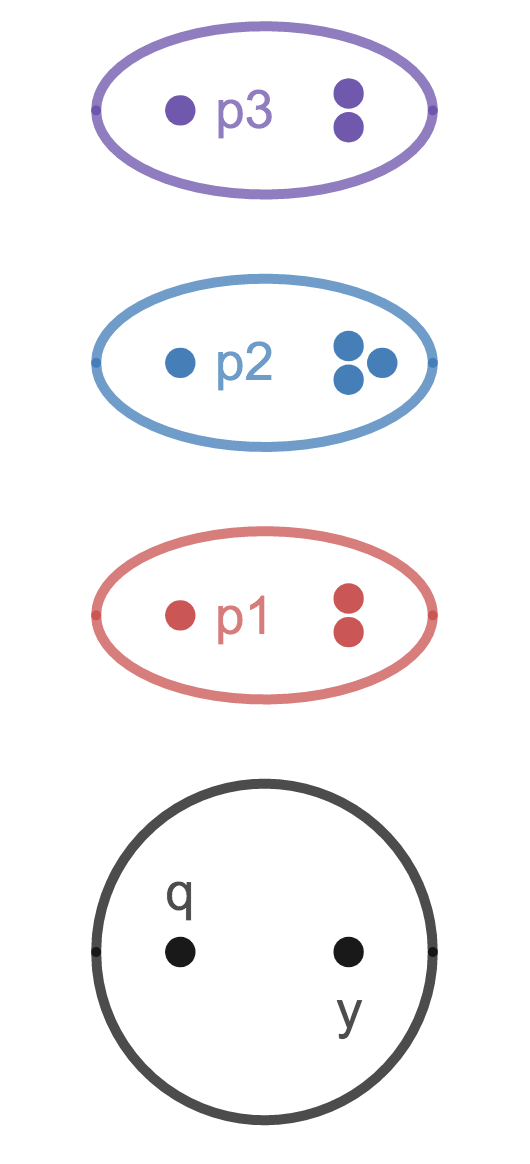
\includegraphics[width=0.2\textwidth]{13.png}
    \caption{Picture to help visualize what's going on with $\deg_q(f)$. Plotted in \cite{Desmos}.}
    \label{fig:Fig13}
\end{figure}
Thus $\deg_q(f) = 7$, and for $y$ near $q$, $\deg_y(f) = 7$, \ita{i.e.}, $y$ gets a distinct preimage for each $e_{p_i}$.

By the above claim, we have shown that $q$ has an open neighborhood on which $\deg_y(f)$ is constant. Let $n := \deg_q(f)$ and let 
\begin{equation}
    S := \setb{y \in Y \mid \deg_y(f) = n}.
\end{equation}
We want to show that $S = Y$, and so $f$ has the same degree \ita{everywhere}. $S \neq \varnothing$ since $q \in S$, and by the above claim $S$ is open. To show that $S$ is closed, let $y_0$ be an accumulation point of $S$, and let $n_0 := \deg_{y_0}(f)$. Then, by the above again, $y_0$ has a neighborhood on which $\deg_y(f)$ is identically equal to $n_0$. But this neighborhood must contain points of $S$ since $y_0$ is an accumulation point of $S$. Hence $n_0 = n$, and so $y_0 \in S$. Thus $S$ is closed, and since $Y$ is connected, $S = Y$. 

So this degree is actually \underline{global}! We can define the \textbf{degree} $\deg f$ of $f$ independent of the choice in $y$. In a sense, $\deg f$ tells us how many points get mapped to the same point in $y$, counting multiplicity of the ramification points.

Now, what happens if we remove the branch points from $Y$ and the ramification points from $X$? The new spaces $X'$ and $Y'$ are still Riemann surfaces, but are no longer compact. Define a new map $\tilde{f} : X' \to Y'$. $\tilde{f}$ is still holomorphic and surjective, but now every point $y \in Y$ has an open neighborhood for which there are $n = \deg f$ disjoint open subsets in $X'$ mapping injectively, and thus homeomorphically, to it. Thus $\tilde{f}$ is a \underline{covering map}, and in particular $X'$ is a $\deg(f)$-fold cover of $Y'$. The original $f$ is called a \textbf{branch cover}, so $f$ is almost a covering map except for those ramification points.
\subsection{Discussion}
Given $X = V(F) \subseteq \p^2$ a nonsingular projective plane curve and the projection map $\pi : [x,y,z] \mapsto [x,z]$ to $\p^1$, how do you determine the degree of $\pi$?

We can look at $V(f) \subseteq \cx^2$, where $f \in \cx[x,y]$ is $F$ dehomogenized at $z$. Then $\pi(x,y) = x$.

Why are we allowed to do this? Since $\deg f$ is defined locally but constant globally, we can work in $U_2$ and know that whatever result we get applies to all of $\p^2$. 

Then for a non-branch point $x_0$, $\deg \pi$ is just the number of preimages of $x_0$, which is the number of solutions of $f(x_0,y) = 0$ for $y$. Thus $\deg \pi$ is the degree of $f$ as a polynomial in $y$.
\subsection{Exercises}
\begin{exercise}
    As we have seen, the rational function 
    \[
        \frac{z^2 + 1}{z}
    \]
    defines a map $\cx_{\infty} \to \cx_{\infty}$ of compact Riemann surfaces. What is its degree? Find the ramification points. Don't forget about $\infty$.
\end{exercise}
\begin{exercise}
    Let $L$ be a lattice in $\cx$, $X = C / L$. Show that $\mu_2 : X \to X$ defined by $\mu_2(x) = 2x$ is well-defined and holomorphic. Find $\deg \mu_2$ and all of the ramification points.
\end{exercise}
\section{March 23}
\subsection{Warmup}
Let $X = V(xz - y^2) \subseteq \p^2$. Let $\pi : X \to \p^1$ be the projection map $\pi : [x,y,z] \to [x,z]$. Find all ramification and branch points. (Start in $U_2$.)

This turned out to be fairly useful to discuss in detail. In $U_2$ the polynomial becomes $x - y^2$, whose graph is easy to understand: 
\begin{figure}[H]
    \centering
    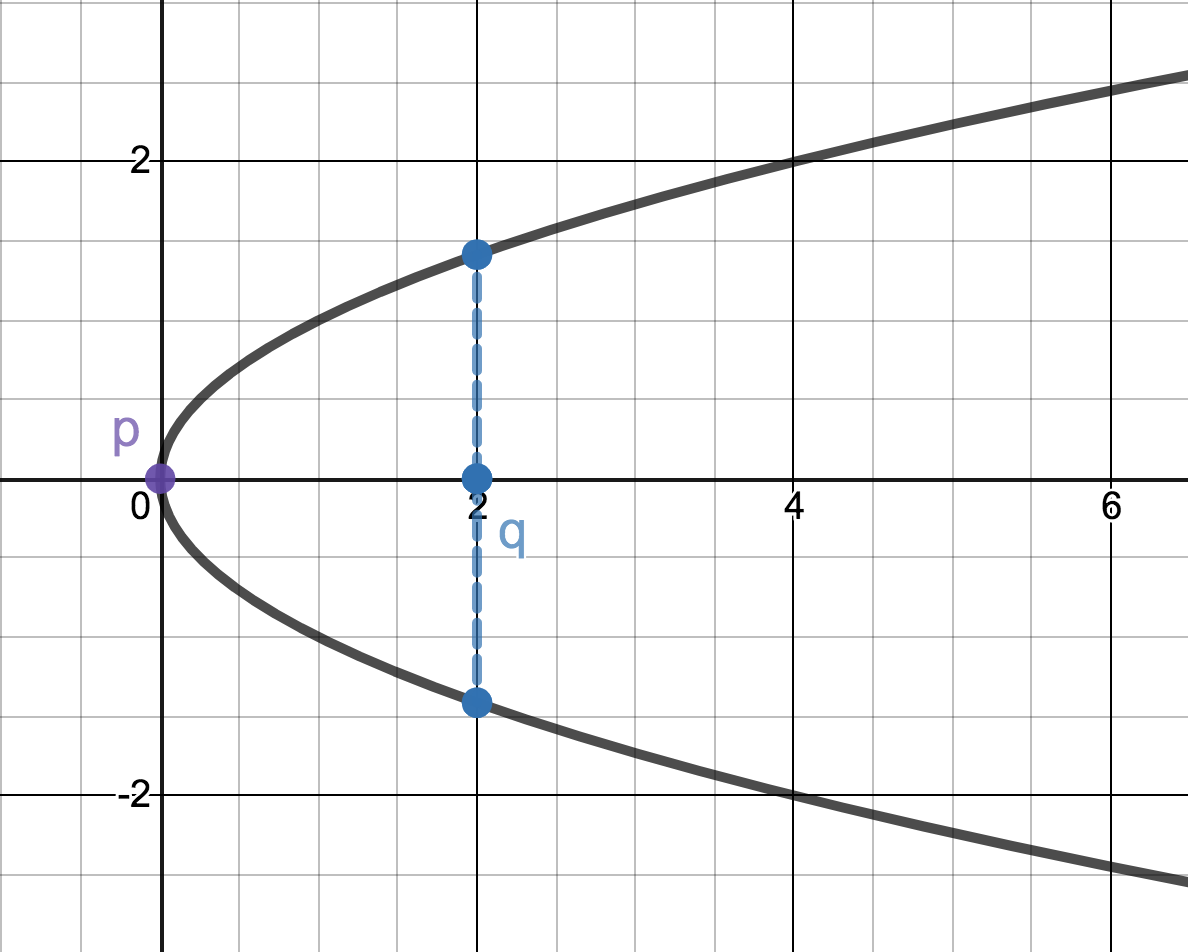
\includegraphics[width = 0.5\textwidth]{14.png}
    \caption{Plotted in \cite{Desmos}.}
    \label{fig:Fig14}
\end{figure}
and projection is simply onto the $x$-axis. Here $q$ is a ``typical'' point, with two preimages, and $p$ evidently has only one; so we expect $p$ to be a ramification point. Indeed, note that at $p$, $x$ is not a chart but $y$ is, so in terms of charts the projection map becomes $y \mapsto x = y^2$, so the ramification index $e_p$ is 2.

The only point not accounted for in $U_2$ comes from setting $z = 0$ and getting $[1,0,0] \in U_0$. In these local coordinates $\pi : (y,z) \mapsto z$ and the local equation for $X$ is $z = y^2$. In other words, the situation at $\infty$ in this case looks just the one at the origin in $U_2$. So there is a second ramification point at the origin in $U_0$ again with ramification index 2. Back in global coordinates, the ramification points are $[0,0,1]$ and $[1,0,0]$ with respective corresponding branch points $[0,1]$ and $[1,0]$ in $\p^1$.
\subsection{More Topology}
Recall that given a compact surface $S$, a \textbf{triangulation} of $S$ is an expression of $S$ is an expression of $S$ as a finite union of \underline{triangles}, each of which consists of a face bounded by three sides with each pair of sides meeting in a vertex and with the property that two triangles meet either in $\varnothing$ or one side or one vertex.
\begin{figure}[H]
    \centering
    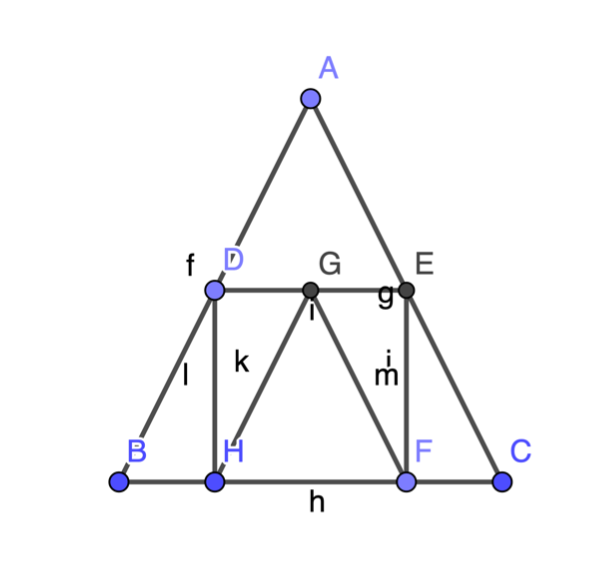
\includegraphics[width = 0.5\textwidth]{15.png}
    \caption{This is not a triangulation, but if we draw a vertical segment from the top vertex down to the middle line, then we get one. Taken from Dr. Brevik's notes. I don't know if I want to make this in Tikz.}
    \label{fig:Fig15}
\end{figure}
\begin{definition}
    Let $S$ be a (compact boundaryless) surface. The \textbf{Euler characteristic} of a particular triangulation $T$ of $S$ is defined as 
    \begin{equation}
        \chi_T := \#\text{ vertices } - \#\text{ edges } + \#\text{ faces for }T.
    \end{equation}
\end{definition}
\begin{example}
    The triangulation $T$ of the sphere as a tetrahedron gives 
    \begin{equation}
        \chi_T = 4 - 6 + 4 = 2.
    \end{equation}
    What if $T$ is the octahedral triangulation?
\end{example}
\begin{theorem}
    For any compact boundaryless surface $S$:
    \begin{itemize}
        \item $S$ has a triangulation.
        \item If a triangulation of $S$ is \underline{refined} by adding vertices and edges and thereby subdividing faces, then the Euler character remains unchanged.
        \item Any two triangulations of $S$ have a common refinement.
    \end{itemize}
\end{theorem}
Therefore we can define unambiguously the Euler characteristic of a compact boundaryless surface $S$ as the Euler characteristic of any of its triangulations.
\begin{definition}
    The \textbf{genus} of $S$ is defined via 
    \begin{equation}
        \chi_S = 2 - 2g_S.
    \end{equation}
\end{definition}
\begin{example}
    Let's find a triangulation of the torus. 
    \begin{figure}[H]
        \centering
        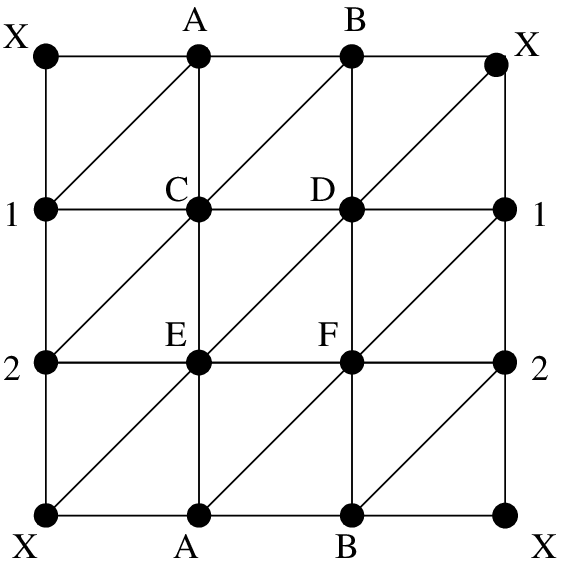
\includegraphics[width = 0.5\textwidth]{16.png}
        \caption{From \url{https://www.researchgate.net/figure/A-triangulation-of-the-torus-Note-that-there-are-18-2-simplices-in-addition-to-the_fig2_48187858}.}
        \label{fig:Fig16}
    \end{figure}
    If you're careful, you'll count 9 vertices (remember the identifications!), 27 vertices, and 18 faces, for an Euler characteristic of 0. This matches with our ``knowledge'' that a torus has genus 1 and the formula $\chi_S = 2 - 2g_S$.
\end{example}
\section{March 25}
\subsection{Morphisms and Genera}
Let $f : X \to Y$ be a nonconstant holomorphic map of Riemann surfaces. We'd like to understand how
\begin{itemize}
    \item the genera $g_X$, $g_Y$ of the two surfaces,
    \item the degree of $f$, and 
    \item the ramification
\end{itemize}
are related.

First, let's think about the case in which $f$ is unramified. What does this mean? $Y$ has an atlas for which the preimage for each chart $V$ has $n$ disjoint components in $X$ mapping homeomorphically to $V$. Triangulate $Y$ in such a way that each triangle lies in one of these charts. Then each triangle has $n = \deg f$ disjoint triangles mapping homeomorphically to it.

The preimages of these triangles form a triangulation of $X$. With this triangulation there are exactly $n$ times as many vertices, edges, and faces as in the one for $Y$. Thus $\chi(X) = n \chi(Y)$ and so 
\begin{equation}
    2 g_X - 2 = n (2g_Y - 2),
\end{equation}
so 
\begin{equation}
    g_X = n g_Y + 1 - n.
\end{equation}
Already, then, we see that there are some pretty serious constraints on the possible genera of $X$ and $Y$ and the degree of $f$ for such a map to be possible.

Now, the ramified case. First, let's think locally: Think of $z \mapsto w = z^r$ as a map from the (closed) unit disk $D$ to itself. If we triangulate $D$ in the $w$-plane, what happens to the Euler characteristic for the induced triangulation of the $z$-disk? 

Now suppose $f : X \to Y$ above does have ramification points. Again triangulate $Y$, but this time make sure that the branch points are all vertices of the triangulation. Let $x \in X$ be a ramification point with ramification index $e = e_x(f)$, and let $y = f(x)$ be the corresponding branch point. Local normal form gives us charts $(U, \varphi)$, $(V, \psi)$ with $x \in U \subseteq X$, $y \in V \subseteq Y$ for which $\psi \circ f \circ \inv{\varphi}$ is the map $z \mapsto z^e$. Shrink $U$ if necessary to guarantee that $f(U) \subseteq V$, and refine the triangulation if necessary so that each triangle involving $y$ is contained in $f(U)$.

Locally we are in the same situation as with the unit disk considered above: suppose that there are $k$ triangles involving $y$, forming a configuration with $k + 1$ vertices, $2k$ edges, and $k$ faces. In the inverse image is a set of $ke$ triangles, with $e$ preimages for each one, and away from $x$ they map as covering spaces. So there are a total of $ke$ faces and $2ke$ edges but only $ke + 1$ vertices. In other words, compared to the unramified case we ``lost'' $e(k+1) - (ke+1) = e-1$ from the Euler characteristic.  Repeat this over all the ramification points and we find that 
\begin{equation}
    \chi(X) = n \chi(Y) - \sum\limits_{x \in X} (e_x - 1),
\end{equation}
and so 
\begin{equation}
    2 g_X - 2 = n (2g_Y - 2) + \sum\limits_{x \in X} (e_x - 1).
\end{equation}
This is the \textbf{Riemann-Hurwitz} formula. As easy corollaries, we note that,
\begin{itemize}
    \item If $f : X \to Y$ is any nonconstant map of compact Riemann surfaces, $g_X \geq g_Y$.
    \item The ramification degree $\sum\limits_{x \in X} (e_x - 1)$ is a nonnegative even integer.
\end{itemize}
In a sense, $n = \deg f$ is almost a ratio of the Euler characteristics of $X$ and $Y$, with correction terms coming from the ramification points.
\subsection{Exercises}
\begin{exercise}
    Show that your solution to Exercise 33 agrees with Riemann-Hurwitz. What can you say about a nonconstant holomorphic map of compact genus-1 Riemann surfaces in general?
\end{exercise}
\begin{exercise}
    Use Riemann-Hurwitz with $X = V(y^2z - x^3 + xz^2)$ and the map $\pi : [x,y,z] \mapsto [x,z]$ studied in earlier examples and Exercise 31 to find $g_X$.
\end{exercise}
\begin{exercise}
    A compact Riemann surface $X$ of genus $g_X \geq 2$ is called \underline{hyperelliptic} if there is a nonconstant holomorphic map $\mu : X \to \p^1$ of degree 2. Find a formula for the number of ramification points of $\mu$ in terms of $g_X$. Explain why degree 2 is necessary for us to be definitive about this number.
\end{exercise}
\begin{exercise}
    Let $d$ be a positive integer and $X = V(x^d + y^d + z^d) \subseteq \p^2$. If you have not done so yet, show that $X$ is a nonsingular projective plane curve; in this case, hand in your write-up separately as Exercise 18. Let $\pi : X \to \p^1$ given by $\pi : [x,y,z] \mapsto [x,z]$. Compute $\deg \pi$, find the ramification points and indices for $\pi$, and use Riemann-Hurwitz to show that $g_X = \frac{(d-1)(d-2)}{2}$. (Hint: $-1$ always has $k$ different $k^{\text{th}}$ roots, no matter what $k$ is.)
    
    [In fact, any two singular projective plane curves of a given degree are homeomorphic, so this genus formula applies to all such curves of degree $d$. I don't think we'll be able to prove that fact, though.]
\end{exercise}
\section{April 6}
\subsection{Curves in Higher Dimensional Spaces}
Not all Riemann surfaces lie in $\cx^2$ or even $\p^1$. For example, let $S$ be the (complex) surface in $\cx^3$ given by $V(x-yz)$, and let $T := V(y - z^2)$. Let $X := S \cap T$. The real-valued part of $S$, $T$, and $X$ in $\real^3$ look something like the following:
\begin{figure}[H]
    \centering
    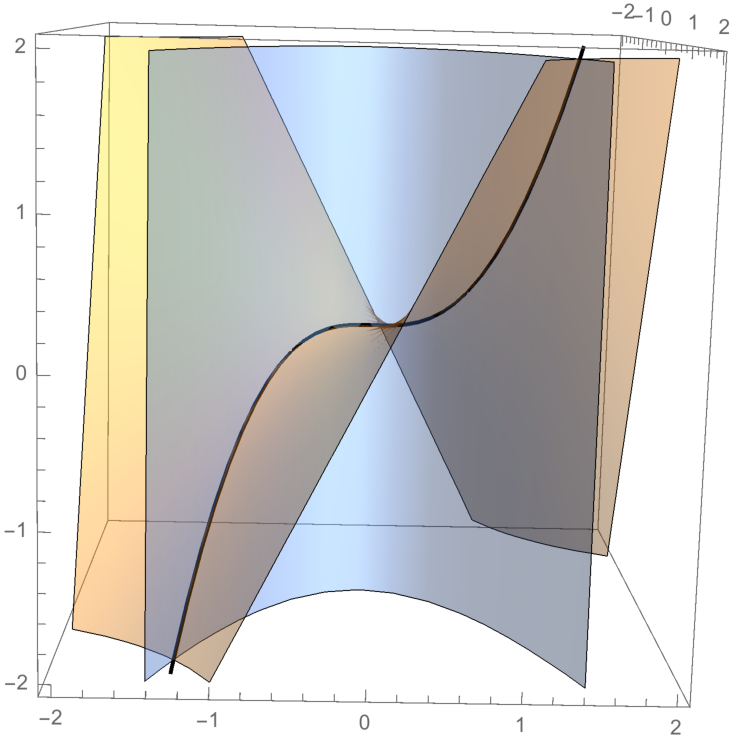
\includegraphics[width=0.5\textwidth]{17.pdf}
    \caption{Real-valued parts of $S$, $T$, and $X$ in $\real^3$. $X$ is the black curve. Plotted in \cite{Mathematica}.}
    \label{fig:Fig17}
\end{figure}
Note that $S$ and $T$ are themselves \ita{not} Riemann surfaces, since they have \underline{complex} dimension 2.

For $(x,y,z) \in X$, $y = z^2$ and $x = yz = z^3$. The $z$-coordinate serves as a chart at every point of $X$, so $X$ can be expressed parametric form as 
\begin{equation}
    \setb{ (t^3 , t^2 , t) \mid t\in \cx}.
\end{equation}
$X$ is sometimes referred to as the \underline{twisted cubic}. Is it a Riemann surface? Since it is the intersection of two complex surfaces, it has complex dimension 1. It's connected since it's the image of $\cx$ under a continuous map, so $X$ is in fact a Riemann surface. In fact $X \cong \cx$. Is it compact? As a subset of $\cx^3$, $X$ is not bounded so no.

Here we say $X$ is called the \textbf{complete intersection} of the two surfaces $S$ and $T$.

Let's compactify $X$ by looking in $\p^3$, where the defining polynomials for $\overline{S}$ and $\overline{T}$ are $xw - yz$ and $yw - z^2$. When $w \neq 0$ we can take $w = 1$, so this gives us back $S$, $T$, and $X$ in $\cx^3$ (really $U_3$). When $w = 0$, then we get the equations $yz = 0$, $z^2 = 0$, so $z = 0$. This leaves $x$ and $y$ free, so we have an entire line, defined by $z = w = 0$ at the infinite points. So in this case $\overline{X} \neq \overline{S} \cap \overline{T}$.

At $U_0$, the polynomials $w - yz$ and $yw - z^2$. In these coordinates, if $z = 0$ then $w = 0$ and this gives us the line from before. Otherwise, substituting gives us $y^2 z = z^2$, which reduces to $y^2 = z$ if $z \neq 0$. Thus away from the line, the curve is given by $z = y^2$, $w = yz = y^3$, so on this piece $y$ serves as a local chart. In fact, these curves look just the ones in $U_3$, just with the variables switched.
\begin{figure}[H]
    \centering
    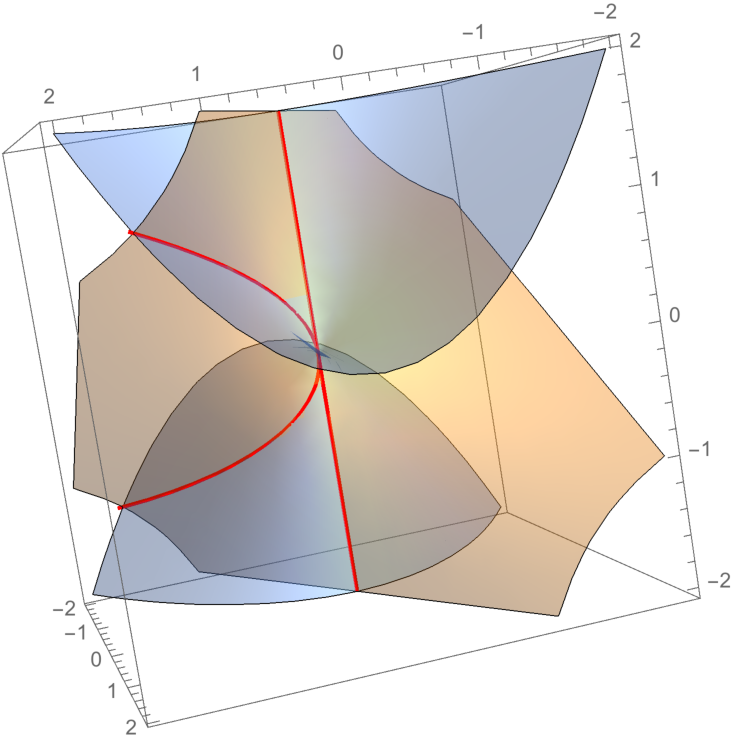
\includegraphics[width=0.5\textwidth]{18.pdf}
    \caption{Real-valued parts of $\overline{S}$, $\overline{T}$, and $\overline{X}$ in the real part of $U_0$. $\overline{X}$ is outlined in red, and notice that it contains an extra line along the $y$-axis (note here that the axes are $y$, $z$, and $w$). Plotted in \cite{Mathematica}.}
    \label{fig:Fig18}
\end{figure}
$\overline{X}$ here is the image of $\p^1$ in $\p^3$ by the ``homogenized'' map $[t,u] \mapsto [t^3 , t^2u , t u^2, u^3]$. The map $\cx \to \cx^3$ discussed above comes from setting $w = 1$ in $\p^3$, which forces $u \neq 0$, so take $u = 1$ for the preimage in $\p^1$. The part of $\overline{X}$ in $U_0$ we get by setting $t = 1$, $x = 1$ so that the map $\cx \to \cx^3$ is $u \mapsto (u , u^2 , u^3)$. Which is why $y$ was the local chart on this piece (or really $\frac{y}{x}$ was a chart on the projective curve). In these coordinates $\overline{X} \cap U_0$ is the complete intersection of the surfaces $V(z - y^2)$ and $V(w - yz)$.

$\overline{X}$ is called the 3-\textbf{uple embedding} of $\p^1$ into $\p^3$, defined as it is by all monomials of degree 3. There is a similar $d$-uple embedding of $\p^1$ into $\p^d$ given by $[t,u] \mapsto [t^d , t^{d-1}u , \dotsc , u^d]$.

Our $\overline{X}$ is \ita{not} the complete intersection of $\overline{S}$ and $\overline{T}$. But any point in $U_3$ has a neighborhood that is the intersection of the appropriate parts of these surfaces. Similarly, any point in $U_0$ has a neighborhood that is the intersection of all parts of $V(z - y^2)$ and $V(w - yz)$. And that accounts for all points of $X$. We say that $\overline{X}$ is a \textbf{local complete intersection}. It is a fact that $\overline{X}$ is \ita{not} a (global) complete intersection: there are no two surfaces in $\p^3$ that cut out $\overline{X}$ precisely. (This fact requires some theory that we don't have.)
\begin{exercise}
    Using the same methods, show that the curve $X \subseteq \p^3$ given by the image of $\phi : \p^1 \to \p^3$ by $\phi : [t,u] \mapsto [t^4 , t^3u , tu^3 , u^4]$ is a local complete intersection. For the two surfaces you find in $U_3$, identify an ``extra'' piece of the intersection of their closures at $\infty$ that shows that $X$ is not the complete intersection of their closures.
\end{exercise}
\subsection{Interlude: \texorpdfstring{$\frac{\partial}{\partial z}$}{d/dz} and \texorpdfstring{$\frac{\partial}{\partial \overline{z}}$}{d/dz}}
Consider an open set $U \subseteq \cx$ and a function $f : U \to \cx$ that is $C^{\infty}$ as a function of two real variables, \ita{i.e.}, if for $z \in U$ we write $z = x + i y$ and we write $f(z) = f(x + i y) = u(x,y) + i v(x,y)$, then $u$ and $v$ have partial derivatives of all orders.

In this setting we define (sensibly)
\begin{equation}
    \begin{split}
        \frac{\partial f}{\partial x} & := f_x := \frac{\partial u}{\partial x} + i \frac{\partial v}{\partial x}, \\ 
        \frac{\partial f}{\partial y} & := f_y := \frac{\partial u}{\partial y} + i \frac{\partial v}{\partial y},
    \end{split}
\end{equation}
Since $z = x + i y$ and $\overline{z} = x - i y$, we can solve for $x$ and $y$:
\begin{equation}
    x = \frac{z + \overline{z}}{2} , \qquad y = \frac{z - \overline{z}}{2i} = -\frac{i}{2} \left( z - \overline{z} \right).
\end{equation}
So we can define (at least symbolically) the following:
\begin{equation}
    \begin{split}
        \frac{\partial f}{\partial z} & = \frac{\partial f}{\partial x} \frac{\partial x}{\partial z} + \frac{\partial f}{\partial y} \frac{\partial y}{\partial z} \\
        & = \frac{1}{2} \left( \frac{\partial u}{\partial x} + i\frac{\partial v}{\partial x} \right) - \frac{i}{2} \left( \frac{\partial u}{\partial y} + i\frac{\partial v}{\partial y} \right) \\
        & = \frac{1}{2} \left[ \left( \frac{\partial u}{\partial x} + \frac{\partial v}{\partial y} \right) + i\left( \frac{\partial v}{\partial x} - \frac{\partial u}{\partial y} \right) \right].
    \end{split}
\end{equation}
Check that the following expressions hold as well: 
\begin{equation}
    \begin{split}
        \frac{\partial f}{\partial \overline{z}} & = \frac{1}{2} \left[ \left( \frac{\partial u}{\partial x} - \frac{\partial v}{\partial y} \right) + i\left( \frac{\partial v}{\partial x} - \frac{\partial u}{\partial y} \right) \right], \\
        \frac{\partial \overline{f}}{\partial z} & = \frac{1}{2} \left[ \left( \frac{\partial u}{\partial x} - \frac{\partial v}{\partial y} \right) - i\left( \frac{\partial v}{\partial x} - \frac{\partial u}{\partial y} \right) \right], \\
        \frac{\partial f}{\partial z} & = \frac{1}{2} \left[ \left( \frac{\partial u}{\partial x} + \frac{\partial v}{\partial y} \right) + i\left( \frac{\partial u}{\partial y} - \frac{\partial v}{\partial x} \right) \right].
    \end{split}
\end{equation}
Note that $f$ satisfies the Cauchy-Riemann equations if and only if $\frac{\partial f}{\partial \overline{z}} = 0$.
\begin{exercise}
    Verify that $\frac{\partial \overline{f}}{\partial z} = \overline{\frac{\partial f}{\partial \overline{z}}}$ and $\frac{\partial \overline{f}}{\partial \overline{z}} = \overline{\frac{\partial f}{\partial z}}$.
\end{exercise}
\begin{exercise}
    \noindent
    \begin{enumerate}[(a)]
        \item Let $f(z) = f(x + iy) = u(x,y) + iv(x,y)$ be a $C^{\infty}$ function on some region $U$ of $\cx$. Let $M$ be the matrix $\begin{bmatrix} 1 & i \\ 1 & -i \end{bmatrix}$. Show that for any point in $U$,
        \[
            M 
            \begin{bmatrix}
                \frac{\partial u}{\partial x} & \frac{\partial u}{\partial y} \\[0.5em]
                \frac{\partial v}{\partial x} & \frac{\partial v}{\partial y}
            \end{bmatrix}
            \inv{M} = 
            \begin{bmatrix}
                \frac{\partial f}{\partial z} & \frac{\partial f}{\partial \overline{z}} \\[0.5em]
                \frac{\partial \overline{f}}{\partial z} & \frac{\partial \overline{f}}{\partial \overline{z}}
            \end{bmatrix}.
        \]
        \item Now suppose that $f_1 = u_1 + iv_1$ and $f_2 = u_2 + iv_2$ are $C^{\infty}$ functions of two complex variables $z_1 = x_1 + iy_1$, $z_2 = x_2 + iy_2$ *so that $u_1$, $v_1$, $u_2$, $v_2$ are functions of four real variables). Find a matrix $A$ that gives a similarity between
        \[
            \begin{bmatrix}
                \frac{\partial u_1}{\partial x_1} & \frac{\partial u_1}{\partial x_2} & \frac{\partial u_1}{\partial y_1} & \frac{\partial u_1}{\partial y_2} \\[0.5em]
                \frac{\partial u_2}{\partial x_1} & \frac{\partial u_2}{\partial x_2} & \frac{\partial u_2}{\partial y_1} & \frac{\partial u_2}{\partial y_2} \\[0.5em]
                \frac{\partial v_1}{\partial x_1} & \frac{\partial v_1}{\partial x_2} & \frac{\partial v_1}{\partial y_1} & \frac{\partial v_1}{\partial y_2} \\[0.5em]
                \frac{\partial v_2}{\partial x_1} & \frac{\partial v_2}{\partial x_2} & \frac{\partial v_2}{\partial y_1} & \frac{\partial v_2}{\partial y_2} 
            \end{bmatrix}
        \]
        and 
        \[
            \begin{bmatrix}
                \frac{\partial f_1}{\partial z_1} & \frac{\partial f_1}{\partial z_2} & 
                \frac{\partial f_1}{\partial \overline{z}_1} &                 \frac{\partial f_1}{\partial \overline{z}_2} \\[0.5em]
                \frac{\partial f_2}{\partial z_1} & \frac{\partial f_2}{\partial z_2} & 
                \frac{\partial f_2}{\partial \overline{z}_1} &                 \frac{\partial f_2}{\partial \overline{z}_2} \\[0.5em]
                \frac{\partial \overline{f_1}}{\partial z_1} & \frac{\partial f_1}{\partial z_2} & 
                \frac{\partial \overline{f_1}}{\partial \overline{z}_1} &                 \frac{\partial \overline{f_1}}{\partial \overline{z}_2} \\[0.5em]
                \frac{\partial \overline{f_2}}{\partial z_1} & \frac{\partial \overline{f_2}}{\partial z_2} & 
                \frac{\partial \overline{f_2}}{\partial \overline{z}_1} &                 \frac{\partial \overline{f_2}}{\partial \overline{z}_2}
            \end{bmatrix}.
        \]
    \end{enumerate}
\end{exercise}
\section{April 8}
\subsection{Local and Global Complete Intersections}
Given two surfaces in $\cx^3$ each defined by a single equation, say $S := V(f)$, $T := V(g)$, their \textbf{complete intersection} is the set $S \cap T$. Generally we reserve this terminology for when $S$ and $T$ don't have any (complex) surface components in common. A curve $X \subseteq \p^3$ is a \textbf{local complete intersection} if every point $p \in X$ has a neighborhood $U$ lying in some copy of $\cx^3$ such there are surfaces $S$ and $T$ such that $X \cap U = S \cap T \cap U$.

We saw last time that the 3-uple embedding $[t,u] \mapsto [t^3,t^2u,tu^2,u^3] \subseteq \p^3$ is a local complete intersection, but not a \underline{global} one.

Can \ita{any} Riemann surface be a global complete intersection? Yes! How about a line? Slightly less trivially, the conic $V(xy - z^2) \subseteq \p^2$ is also the intersection of the \underline{surface} with that same equation in $\p^3$ and the plane $w = 0$. But a complete intersection is not always a Riemann surface! Intersect that same surface $V(xy - z^2) \subseteq \p^3$ with the plane $z = 0$ instead. We get $V(xy)$, the union of two lines meeting at a point, which is not a Riemann surface.

Similarly, one can ask about local and global complete intersections in bigger spaces. In general, a Riemann surface $X$ is a local complete intersection in $\cx^n$ or $\p^n$ if around each point one can find $n-1$ hypersurfaces, each defined by a single polynomial, that cut out $X$ in a neighborhood of that point.
\begin{exercise}
    Show that the 4-uple embedding of $\p^1$ into $\p^4$ is a local complete intersection. (As before you will only need to consider two open sets for this one.)
\end{exercise}
Quick aside, given a Riemann surface $X \subseteq \p^n$ with genus 2, is there an $f : \p^1 \to \p^n$ such that $f(\p^1) = X$? No, we can't increase the genus! This can be made precise by using Riemann-Hurwitz. So most of the time, we won't get a nice parametric map for $X$.

Just as with plane curves, not all local complete intersections are Riemann surfaces. For plane curves we found a nice criterion if one of the partials at a point is nonvanishing, the other variable is a chart near that point. This was where the Implicit Function Theorem came in. Similarly, given a local complete intersection in higher dimensions, can we find an analogous Implicit Function Theorem to help us find a coordinate giving a chart near a point?
\subsection{Digression: Inverse and Implicit Function Theorems}
\begin{remark}
    This material is mostly lifted from Spivak's classic \ita{Calculus on Manifolds}. 
\end{remark}
\begin{definition}
    Let $U \subseteq \real^n$ be open, $f : U \to \real$, $a \in U$. A \textbf{derivative} of $f$ at $a$ is a \underline{linear function} $\lambda : \real^n \to \real$ such that 
    \begin{equation}
        \lim\limits_{x \to a} \frac{| f(x) - f(a) - \lambda(x - a) |}{| x - a |} = 0.
    \end{equation}
    (Note the necessity of using $|\,|$ here, which in the denominator is interpreted to be the Euclidean norm.) If $f$ has a derivative at $a$, we say that $f$ is \textbf{differentiable at $a$}. We write $\lambda = f'(a)$ once we establish that $\lambda$ is unique!
\end{definition}
\begin{remark}
    \noindent
    \begin{itemize}
        \item If $\lambda$ exists, then it is unique: suppose that $\mu$ is another derivative of $f$ at $a$. Then
        \begin{equation}
            \begin{split}
                \frac{|(\mu - \lambda)(x - a)|}{|x-a|} & = \frac{|\mu(x-a) - \lambda(x-a)|}{|x-a|} \\
                & \leq \frac{|f(x) - f(a) - \lambda(x-a)|}{|x-a|} + \frac{\left|\mu(x-a) - \left( f(x) - f(a) \right) \right|}{|x -a |} \\
                & \to 0
            \end{split}
        \end{equation}
        as $x \to a$. The only way this can happen is if $\mu - \lambda$ is the 0 linear transformation, because $\mu - \lambda$ is linear, and thus if there were any $v \in \real^n$ for which $(\lambda - \mu)(v) \neq 0$, then 
        \begin{equation}
            \begin{split}
                \lim\limits_{t \to 0} \frac{|(\mu - \lambda)(a + tv - a)|}{|a + tv - a|} & = \frac{| (\mu - \lambda)(tv) |}{|tv|} \\
                & = \frac{|(\mu - \lambda)(v)|}{|v|} \\
                & \neq 0.
            \end{split}
        \end{equation}
        \item A \underline{derivative} of $f$ at $a$ is a \underline{linear function} $\lambda : \real^n \to \real$. In the case of 1 variable, of course we are used to thinking of the derivative as a number, but in this way of looking at things it's really the linear approximation. How do the number and the linear approximation relate?
        
        Since the derivative is linear, we can represent it as a matrix. What is the matrix (relative to the standard basis)? If all of the first order partials of $f$ exist, then it's the $1 \times n$ matrix of these derivatives of $f$ evaluated at $a$:
        \begin{equation}
            \lambda = \left. \left( \frac{\partial f}{\partial x_1} , \dotsc , \frac{\partial f}{\partial x_n} \right) \right|_{x = a} : \real^n \to \real.
        \end{equation}
        In vector calculus, the corresponding $n \times 1$ column vector would be called the \textbf{gradient} of $f$ at $a$. Note that since we're writing the derivative as a row vector, we're treating it as a dual vector. We call this the \textbf{Jacobian matrix} of $f$ at $a$.
    \end{itemize}
\end{remark}
The concept generalizes easily to higher dimensions: let $U \subseteq \real^n$ be open, $a \in U$, $f : U \to \real^m$. Then $f$ is defined by its coordinate functions $f_1 , \dotsc , f_m : \real^n \to \real$. Thus the derivative is a linear transformation $\real^n \to \real^m$ consisting of the separate derivatives going to the different coordinates in $\real^n$. The corresponding matrix is the \textbf{Jacobian matrix}
\begin{equation}
    J_f(a) = 
    \begin{bmatrix}
        \frac{\partial f_1}{\partial x_1} & \frac{\partial f_1}{\partial x_2} & \cdots & \frac{\partial f_1}{\partial x_n} \\
        \vdots & \vdots & \ddots & \vdots \\
        \frac{\partial f_m}{\partial x_1} & \frac{\partial f_m}{\partial x_2} & \cdots & \frac{\partial f_m}{\partial x_n}
    \end{bmatrix}, 
    \qquad
    \left( J_f(a) \right)_{ij} = \frac{\partial f_i}{\partial x_j},
\end{equation}
with the derivatives all evaluated at $a$. Note that this is just the matrices for the individual derivatives of the $f_i$'s stacked on top of one another.
\begin{example}
    Let $f(x,y) = (x^2y, x \sin y , 2x \cos y)$. Find $J_f(2,0)$ and use it to estimate $f(1.9,0.2)$.
\end{example}
\begin{remark}
    \noindent
    \begin{itemize}
        \item If $f : U \to \real^m$ is a linear map itself, then $f'(a) = f$ at every $a \in U$. Thus ``a linear function is its own derivative.'' Sort of!
        \item Differentiation is linear in the usual senses: $(f + g)' = f' + g'$ and $(cf)' = cf'$ for all differentiable $f , g$ and all $c \in \real$.
    \end{itemize}
\end{remark}
\begin{exercise}
    Prove the \underline{Chain Rule}: Let $U$ be an open set of $\real^n$, $a \in U$, $f : U \to \real^m$, $V \subseteq \real^m$ an open set containing $f(a)$, $g : V \to \real^p$. Prove that if $f$ is differentiable at $a$ and $g$ is differentiable at $f(a)$, then $g \circ f$ is differentiable at $a$ and $J_{g \circ f}(a) = J_g \left( f(a) \right) J_f(a)$.
\end{exercise}
\section{April 13}
\subsection{Real and Complex Derivatives}
Recall that in recent homework exercises, for $f = u(x,y) + i v(x,y)$ a $C^{\infty}$ function of a complex variable $z$ we defined by partial derivatives $\frac{\partial f}{\partial z}$ and $\frac{\partial f}{\partial \overline{z}}$. We showed that $f$ satisfies the Cauchy-Riemann equations if and only if $\frac{\partial f}{\partial \overline{z}} = 0$. Thus for $f$ analytic on some domain, $\frac{\partial f}{\partial \overline{z}}$ identically zero, the Cauchy-Riemann equations are also equivalent to 
\begin{equation}
    \frac{\partial f}{\partial z} = \frac{1}{2} \left[ \left( \frac{\partial u}{\partial x} + \frac{\partial v}{\partial y} \right) + i \left( \frac{\partial v}{\partial x} - \frac{\partial u}{\partial y} \right) \right]
\end{equation}
being equal to 
\begin{equation}
    \frac{\partial u}{\partial x} + i \frac{\partial v}{\partial x} = f'(z).
\end{equation}
So if $f$ is analytic in a domain, $f'(z) = \frac{\partial f}{\partial z}$.

We also saw in a recent exercise that for $f$ a $C^{\infty}$ function of $z$, there is a (constant) matrix $M$ such that 
\begin{equation}
    M 
    \begin{bmatrix}
        \frac{\partial u}{\partial x} & \frac{\partial u}{\partial y} \\[0.5em]
        \frac{\partial v}{\partial x} & \frac{\partial v}{\partial y}
    \end{bmatrix}
    \inv{M} = 
    \begin{bmatrix}
        \frac{\partial f}{\partial z} & \frac{\partial f}{\partial \overline{z}} \\[0.5em]
        \frac{\partial \overline{f}}{\partial z} & \frac{\partial \overline{f}}{\partial \overline{z}}
    \end{bmatrix},
\end{equation}
and we found another matrix $A$ that did an analogous thing for two functions $f_1$, $f_2$ of two variables ($z_1$ and $z_2$). In block-form shorthand it looks like \begin{equation}
    A 
    \left[
        \def\arraystretch{1.5}
        \begin{array}{c | c}
            \frac{\partial u}{\partial x} & \frac{\partial u}{\partial y} \\
            \hline 
            \frac{\partial v}{\partial x} & \frac{\partial v}{\partial y}
        \end{array}
    \right]
    \inv{A} 
    = 
    \left[
        \def\arraystretch{1.5}
        \begin{array}{c | c}
            \frac{\partial f}{\partial z} & \frac{\partial f}{\partial \overline{z}} \\
            \hline 
            \frac{\partial \overline{f}}{\partial z} & \frac{\partial \overline{f}}{\partial \overline{z}}
        \end{array}
    \right]
\end{equation}
where $\left( \frac{\partial u}{\partial x} \right)$ stands for 
\begin{equation}
    \left[
        \def\arraystretch{1.5}
        \begin{array}{c | c}
            \frac{\partial u_1}{\partial x_1} & \frac{\partial u_1}{\partial x_2} \\
            \hline 
            \frac{\partial u_2}{\partial x_1} & \frac{\partial u_2}{\partial x_2}
        \end{array}
    \right]
\end{equation}
and \ita{etc}. There is an analogous similarity with $n$ $C^{\infty}$ functions of $n$ complex variables.

$M$ was given by 
\begin{equation}
    M = 
    \begin{bmatrix}
        1 & i \\
        1 & -i
    \end{bmatrix}.
\end{equation}
Note that $M$ is \ita{almost} unitary:
\begin{equation}
    \begin{split}
        M M^* & = 
        \begin{bmatrix}
            1 & i \\
            1 & -i
        \end{bmatrix}
        \begin{bmatrix}
            1 & i \\
            1 & -i
        \end{bmatrix}^* \\
        & =
        \begin{bmatrix}
            1 & i \\
            1 & -i
        \end{bmatrix}
        \begin{bmatrix}
            1 & 1 \\
            -i & i
        \end{bmatrix} \\
        & = 
        \begin{bmatrix}
            2 & 0 \\
            0 & 2
        \end{bmatrix}.
    \end{split}
\end{equation}
Redefining $M$ up to a constant scaling will give us a unitary matrix.

In fact, the matrix $A$ is in general given by 
\begin{equation}
    A = I_n \otimes M,
\end{equation}
where $I_n$ is the $n \times n$ identity matrix and $\otimes$ is the standard matrix Kronecker product. Notice that $A$ is \ita{almost} unitary for the same reason that $M$ was:
\begin{equation}
    \begin{split}
        A A^* & = \left( I_n \otimes M \right) \left( I_n \otimes M \right)^* \\
        & = \left( I_n \otimes M \right) \left( I_n^* \otimes M^* \right) \\
        & = \left( I_n \otimes M \right) \left( I_n \otimes M^* \right) \\
        & = \left( I_n I_n \right) \otimes \left( M M^* \right) \\
        & = I_n \otimes 2 I_2 \\
        & = 2 I_{2n}.
    \end{split}
\end{equation}

Suppose that $f_1 , \dotsc , f_n$ are functions of $n$ complex variables $z_1 , \dotsc , z_n$ with $x_j, y_j, u_j, v_j$ defined as usual. The matrix
\begin{equation}
    \left[
        \def\arraystretch{1.5}
        \begin{array}{c | c}
            \frac{\partial u}{\partial x} & \frac{\partial u}{\partial y} \\
            \hline 
            \frac{\partial v}{\partial x} & \frac{\partial v}{\partial y}
        \end{array}
    \right]
\end{equation}
is the Jacobian for the real functions $u_1 , \dotsc , u_n$, $v_1 , \dotsc , v_n$ of the $2n$ real variables $x_1 , \dotsc , x_n$, $y_1 , \dotsc , y_n$ in those orders. Now suppose that the $f_1 , \dotsc , f_n$ are \underline{holomorphic} functions on some domain. In that case the right-hand side of the similarity simplifies to 
\begin{equation}
    \left[
        \def\arraystretch{1.5}
        \begin{array}{c | c}
            \frac{\partial f}{\partial z} & 0 \\
            \hline 
            0 & \overline{\frac{\partial f}{\partial z}}
        \end{array}
    \right]
\end{equation}
and so taking determinants of both sides gives us that the Jacobian has real determinant:
\begin{equation}
    \det 
    \left[
        \def\arraystretch{1.5}
        \begin{array}{c | c}
            \frac{\partial u}{\partial x} & \frac{\partial u}{\partial y} \\
            \hline 
            \frac{\partial v}{\partial x} & \frac{\partial v}{\partial y}
        \end{array}
    \right]
    = 
    \left| \det \left( \frac{\partial f}{\partial z} \right) \right|^2.
\end{equation}
(Note that taking the determinant of a direct sum of matrices is just the product of the determinants.) In fact this determinant is nonnegative, and this corresponds to $f$ being holomorphic and thus \underline{conformal}, which means $f$ preserves orientation.
\subsection{Inverse Function Theorem}
\begin{lemma}
    Let $U \subseteq \real^n$ be an open rectangle, $f = (f_1 , \dotsc , f_n) : U \to \real^n$ differerentiable at $a \in U$, and suppose that there exists $M > 0$ such that $\left| D_j f_i (x) \right| \leq M$ for all $i, j \in \oneton$ and for all $x \in U$. Then for all $x , y \in U$, $|f(y) - f(x)| \leq n^2 M |y - x|$.
\end{lemma}
\begin{remark}
    $D_j f_i$ is shorthand for $\frac{\partial f_i}{\partial x_j}$.
\end{remark}
\begin{proof}
    Let $x , y \in U$; write $x = (x_1 , \dotsc , x_n)$, $y = (y_1 , \dotsc , y_n)$. Then for each $i \in \oneton$, 
    \begin{equation}
        \begin{split}
            f_i(y) - f_i(x) & = f_i(y_1 , y_2 , \dotsc , y_n) - f_i(x_1 , x_2,  \dotsc , x_n) \\
            & = f_i(y_1 , y_2 , \dotsc , y_n) - f_i(x_1 , y_2 , \dotsc , y_n) \\
            & + f_i(x_1 , y_2 ,  \dotsc , y_n) - f_i(x_1 , x_2, y_3 , \dotsc , x_n) \\
            & + \dotsb \\
            & + f_i(x_1 , x_2 ,\dotsc , x_{n-1} , y_n) - f_i(x_1 , x_2, \dotsc , x_{n-1} , x_n).
        \end{split}
    \end{equation}
    By the Mean Value Theorem there exists $z_{ij}$ between $x_j$ and $y_j$ such that this sum is equal to 
    \begin{equation}
        \sum\limits_{j = 1}^n D_j f_i (y_1 , \dotsc , y_{j-1} , z_{ij} , x_{j+1} , \dotsc , x_n) (y_i - x_j),
    \end{equation}
    which is then $\leq n M |y-x|$ in absolute value. Finally
    \begin{equation}
        |f(y) - f(x)| \leq \sum\limits_{i = 1}^n |f_i(y) - f_i(x)| \leq n^2 M |y-x|.
    \end{equation}
\end{proof}

\section{April 15}
\subsection{Inverse Function Theorem}
\begin{theorem}[Inverse Function Theorem]
    Let $U \subseteq \real^n$ be an open set, $f : U \to \real^n$ continuously differentiable (meaning that the partial derivatives $D_jf_i$ are continuous for all $1 \leq i , j \leq n$) on $U$. Suppose that for some $a \in U$, $J_f(a)$ has a nonzero determinant. Then there is an open set $V$ containing $a$ such that $f \mid_V : V \to f(V)$ is bijective onto an open set of $\real^n$. Moreover, $\inv{f}$ is differentiable with derivative $D_{\inv{f}}(y) = \inv{ \paren{ D_f \paren{ \inv{f}(y) } } }$ for all $y \in f(V)$.
\end{theorem}
\begin{proof}
    First, note that the theorem is true for linear transformations. Now we're going to make a reduction. Form $\inv{ \paren{ D_f(a) } }$ and then make the composition $\inv{ \paren{ D_f(a) } } \circ f$. This is a differentiable map whose derivative at $a$ is the identity transformation. (Why? Because the derivative of a linear transformation is that same transformation everywhere; now use the Chain Rule.) If the theorem is true for this composition, it's also true for the original $f$, since we can just compose again with $D_f(a)$.
    
    We claim that there is a (closed) rectangle $V$ containing $a$ such that $f(x) \neq f(a)$ for all $x \in V \setminus \setb{ a }$: for $x \neq a$ such that $f(x) = f(a)$, then 
    \[
        \frac{ | f(x) - f(a) - (x - a) | }{|x - a|} = 1.
    \]
    Since $D_f(a)$ is the identity matrix $I_n$,
    \[
        \lim\limits_{x \to a} \frac{ | f(x) - f(a) - (x - a) | }{|x - a|}  = \lim\limits_{x \to a} \frac{ | f(x) - f(a) - D_f(a)(x - a) | }{|x - a|}  = 0.
    \]
    So we have a neighborhood of $a$ such that $f(x) \neq f(a)$ on that neighborhood. 
    
    Next, there is a rectangle $V'$ containing $a$ such that for all $x \in V'$,
    \begin{enumerate}[(i)]
        \item $\det J_f(x) \neq 0$ (this follows from $\det$ being continuous and $f$ being continuously differentiable), and
        \item $|D_jf_i(x) - D_jf_i(a)| \leq \frac{1}{2n^2}$ for all $1 \leq i , j \leq n$.
    \end{enumerate}
    Now shrink $V$ if necessary so that it lies in $V'$. Since $D_f(a) = I_n$, $D_jf_i(a) = \delta_{ij}$ (Kronecker delta!). Let $g(x) := f(x) - x$. Since 
    \[
        D_jg_i(x) = D_jf_i(x) - \delta_{ij} = D_jf_i(x) - D_jf_i(a),
    \]
    $|D_jg_i(x)| \leq \frac{1}{2n^2}$ for all $x \in V$. Let $x_1 , x_2 \in V$. Then by the lemma from last time, 
    \begin{align*}
        \left| f(x_2) - x_2 - \paren{f(x_1) - x_1} \right| & = |g(x_2) - g(x_1)| \\
        & \leq n^2 \cdot \frac{1}{2n^2}|x_2 - x_1| \\
        & = \frac{1}{2}|x_2 - x_1|.
    \end{align*}
    By the Triangle Inequality, for any $x_1 , x_2 \in V$, 
    \[
        |x_1 - x_2| - |f(x_2) - f(x_1)| \leq \left| f(x_2) - x_2 - \paren{f(x_1) - x_1} \right|.
    \]
    So put this together with the previous inequality to get 
    \[
        |x_1 - x_2| - |f(x_2) - f(x_1)| \leq \frac{1}{2}|x_2 - x_1|.
    \]
    Rearrange terms to conclude that 
    \[
        2|f(x_2) - f(x_1)| \leq |x_2 - x_1|
    \]
    for all $x_1 , x_2 \in V$.
    
    Since the boundary $\partial V$ of $V$ is compact, so is $f(\partial V)$, and $f(a) \notin f(\partial V)$ by the uniqueness we established above, so there exists $\delta > 0$ such that $|f(x) - f(a)| > \delta$ for all $x \in \partial V$. Let 
    \[
        W := \setb{ y \in \real^n \, \middle| \, |y - f(a)| < \frac{\delta}{2} }.
    \]
    Now let $y = (y_1 , \dotsc , y_n) \in W$; we claim that there exists a unique $x \in V^{\circ}$ (interior of $V$) such that $f(x) = y$.
    \begin{enumerate}[(i)]
        \item For existence, let 
        \[
            d(x) := |y - f(x)|^2 = \sum\limits_{i = 1}^n \paren{ y_j - f_i(x) }^2.
        \]
        $d$ is continuous and since $V$ is compact (closed and bounded, so thanks Heine-Borel), $d$ has a minimum on $V$. Furthermore, for $x \in \partial V$, $|f(a) - y| < \frac{\delta}{2}$ and $|f(x) - a| > \delta$, so 
        \[
            |f(x) - y| \geq |f(x) - f(a)| - |y - f(a)| \geq \frac{\delta}{2}.
        \]
        So $d(a) < d(x)$ and therefore $d$ does not attain its minimum on $\partial V$. Thus $d$ attains its minimum at a critical point, since $d$ is differentiable on $V$. Let $x_0$ be this point; then for each $j$,
        \[
            D_jd(x_0) - \sum\limits_{i = 1}^n \paren{ y_i - f_i(x_0) } D_j(f_i)(x_0) = 0.
        \]
        Since $\det J_f(x_0) \neq 0$, the columns of $D_jf_i(x_0)$ are linearly independent, so the coefficients $2(y_i - f_i(x_0)$ must all be zero. Thus $f(x_0) = y$, and this proves existence.
        \item For uniqueness, suppose that $f(x_0) = f(x_1) = y$ (say). Then $0 \leq |x_1 - x_0|$ so $x_0 = x_1$.
    \end{enumerate}
    Therefore $f$ gives a bijection between a revised $U := V^{\circ} \cap \inv{f}(W)$ and $W$.
    
    To show continuity, we just use the inequality $2|f(x_2) - f(x_1)| \geq |x_2 - x_1|$. Let $y_1 , y_2 \in f(U)$, then $y_i = f(x_i)$ for some $x_i \in U$. Then 
    \begin{align*}
        \left| \inv{f}(y_2) - \inv{f}(y_1) \right| & = |x_2 - x_1| \\
        & \leq 2 |f(x_2) - f(x_1)| \\
        & = 2 |y_1 - y_2|.
    \end{align*}
    Thus $\inv{f}$ is in fact Lipschitz, and so is continuous. 
    
    It remains to show that $\inv{f}$ is differentiable with the claimed derivative. Let $c \in W$, $b := \inv{f}(c)$. Note that since $f$ is differentiable at $b$, for any $x \in U$ we can write
    \[
        f(x) = f(b) + A(x-b) + \phi(x),
    \]
    where 
    \[
        \lim\limits_{x \to b} \frac{|\phi(x)|}{|x - b|} = 0,
    \]
    and where $A := D_f(b)$ is linear and invertible. For any $y \in W$ there exists a unique $x \in U$ for which $f(x) = y$ and so 
    \[
        y = c + A \paren{ \inv{f}(y( - \inv{f}(c) } + \phi \paren{ \inv{f}(y) },
    \]
    and since $\inv{f}$ is continuous, 
    \[
        \lim\limits_{y \to c} \frac{ \left| \phi \paren{ \inv{f}(y) } \right| }{ \left| \inv{f}(y) - \inv{f}(c) \right| } = 0.
    \]
    Rearrange the terms in the previous equation to get
    \[
        A \paren{ \inv{f}(y) - \inv{f}(c) } - (y - c) = \phi \paren{ \inv{f}(y) }.
    \]
    Hit both sides with $\inv{A}$:
    \[
        \inv{f}(y) - \inv{f}(c) - \inv{A}(y - c) = -\phi \paren{ \inv{f}(y) },
    \]
    so 
    \[
        \lim\limits_{y \to c} \frac{ \left| \inv{f}(y) - \inv{f}(c) - \inv{A}(y - c) \right| }{ \left| \inv{f}(y) - \inv{f}(c) \right|} = 0.
    \]
    Now, for all $y \in W$, 
    \[
        \frac{ \left| \inv{f}(y) - \inv{f}(c) \right| }{\left| y - c \right|} \leq 2,
    \]
    so 
    \[
        \lim\limits_{y \to c} \frac{ \left| \inv{f}(y) - \inv{f}(c) - \inv{A}(y - c) \right| }{\left| y - c \right|} = 0,
    \]
    and therefore $\inv{f}$ is differentiable at $c = f(b)$ with derivative $D_f(c) = \inv{ \paren{ D_f(b) } }$.
\end{proof}
\section{April 20}
What's purple and works from home? A non-abelian grape.
\subsection{Complex Inverse Function Theorem}
From last time we proved the real variables version of the Inverse Function Theorem. Now we'd like to build a complex version. Our setup will be analogous, with $n$ functions on an open subset of $\cx^n$. And we'll leverage the theorem we just proved.
\begin{theorem}[Inverse Function Theorem]
    Let $U \subseteq \cx^n$ be an open set, $f : U \to \cx^n$ holomorphic on $U$. Suppose that for some $a \in U$ the complex Jacobian $J_f(a)$ has nonzero determinant. Then there is an open set $V$ containing $a$ such that $f|_V : V \to f(V)$ is bijective onto an open set of $\cx^n$. Moreover, $\inv{f}$ is holomorphic with derivative $D_{\inv{f}}(w) = \inv{ \paren{ D_f \paren{ \inv{f}(w) } } }$ for all $w \in f(V)$.
\end{theorem}
A note on Jacobians: $J_g$ will be the Jacobian for any function $g$, real or complex. Write each $z_k$ as $x_k + i y_k$, and each $f_j$ as $u_j + iv_j$. Then each of the $u_j$ and $v_j$ are continuously differentiable ($C^{\infty}$) functions of the $2n$ (real) variables $x_1 , \dotsc , x_n , y_1 , \dotsc , y_n$.
\begin{proof}
    First, forget the complex structure, regarding $\cx^n$ as $\real^{2n}$. Let $f_{\real} : U \to \real^{2n}$ be the resulting function written so:
    \[
        \begin{bmatrix}
            u_1 \paren{ x_1 , x_2 , \dotsc , x_n , y_1 , y_2 , \dotsc , y_n } \\
            \vdots \\
            u_n \paren{ x_1 , x_2 , \dotsc , x_n , y_1 , y_2 , \dotsc , y_n } \\
            v_1 \paren{ x_1 , x_2 , \dotsc , x_n , y_1 , y_2 , \dotsc , y_n } \\
            \vdots \\
            v_n \paren{ x_1 , x_2 , \dotsc , x_n , y_1 , y_2 , \dotsc , y_n }
        \end{bmatrix}.
    \]
    When we write $f_{\real}$, we saw that there is a particular matrix $A \in GL_n(\cx)$ such that 
    \[
        A J_{f_{\real}} \inv{A} = 
        \left[ 
            \def\arraystretch{1.5}
            \begin{array}{c|c}
                J_f & 0 \\
                \hline
                0 & \overline{J_f}
            \end{array}
        \right].
    \]
    Since $\det \paren{ J_f(a) } \neq 0$, the determinant of the block matrix on the RHS is 
    \[
        \det \paren{ J_f(a) } \overline{ \det \paren{ J_f(a) } } = \left| \det \paren{ J_f(a) } \right|^2 \neq 0.
    \]
    So then $\det \paren{ J_{f_{\real}}(a) } \neq 0$ as well, so the real Inverse Function Theorem applies to $f_{\real}$, so there is an open set $V$ containing $a$ such that $f_{\real} |_V : V \to f_{\real}(V)$ is bijective onto an open set of $\real^{2n}$, and $\inv{f_{\real}}$ is continuously differentiable. 
    
    Recall that in general, for $P, M \in GL_n(k)$, $\inv{ \paren{P M \inv{P} } } = P \inv{M} \inv{P}$. Therefore for all $w \in f(V)$,
    \begin{align*}
        A J_{ \inv{ f_{\real} } } \inv{A} & = A \inv{ \paren{ J_{ f_{\real} } \paren{ \inv{f}(w) } } } \inv{A} \\
        & = \inv{ \paren{ A J_{f_{\real}} \paren{ \inv{f}(w) } \inv{A} } } \\
        & = \inv{ \left[ 
            \def\arraystretch{1.5}
            \begin{array}{c|c}
                J_f \paren{ \inv{f}(w) } & 0 \\
                \hline
                0 & \overline{J_f \paren{ \inv{f}(w) } }
            \end{array}
        \right] } \\
        & = \left[ 
            \def\arraystretch{1.5}
            \begin{array}{c|c}
                \inv{ J_f \paren{ \inv{f}(w) } } & 0 \\
                \hline
                0 & \inv{ \overline{J_f \paren{ \inv{f}(w) } } }
            \end{array}
        \right].
    \end{align*}
    Let $g := \inv{f}$. Since $f_{\real}$ took real inputs first and gave the real outputs first, $g$ does the same, and so $g_{\real} = \inv{f_{\real}}$. So now for all $w \in f(V)$,
    \[
        A J_{g_{\real}} \paren{ \inv{f}(w) } \inv{A} = 
        \left[ 
            \def\arraystretch{1.5}
            \begin{array}{c|c}
                \inv{ J_f \paren{ \inv{f}(w) } } & 0 \\
                \hline
                0 & \inv{ \overline{J_f \paren{ \inv{f}(w) } } }
            \end{array}
        \right].
    \]
    But recall that $A$ is the \underline{magic matrix} with the property that
    \[
        A J_{g_{\real}} \inv{A} = 
        \left[ 
            \def\arraystretch{1.5}
            \begin{array}{c|c}
                \frac{\partial g}{\partial z}(w) & \frac{\partial g}{\partial \overline{z}}(w) \\
                \hline
                \frac{\partial \overline{g}}{\partial z}(w) & \frac{\partial \overline{g}}{\partial \overline{z}}(w)
            \end{array}
        \right].
    \]
    Then the off-diagonal blocks vanish, which is equivalent to $g$ satisfying the Cauchy-Riemann equations, and so $g$ is holomorphic on $V$! Then the upper-left block is the complex Jacobian of $g$, so 
    \[
        D_g(w) = \inv{ \paren{ D_f \paren{ \inv{f}(w) } } }
    \]
    for all $w \in f(V)$.
\end{proof}
\subsection{Implicit Function Theorem}
As mentioned when we started this particular adventure, we really want a multivariable Implicit Function Theorem that can give us conditions for which a given (local) complete intersection $X \subseteq \cx^n$ or $\p^n$ has a coordinate chart in a neighborhood of a given point $p \in X$. In other words, near $p$ is there a coordinate $x_j$ such that $x_j$ defines \ita{each} of the other $x_k$ on $X$? Just as for plane curves, such a condition would help us determine whether the whole thing is a Riemann surface.

Recall that for a plane curve $X = V(f) \subseteq \cx^2$, $p \in X$, the criterion to determine whether $X$ is \ita{locally} a Riemann surface near $p$ was that one of the partial derivatives $f_x$, $f_y$ needed to to be nonzero. Then the \ita{other} coordinate function can be used as a chart near $p$.

In our new setting, $X \subseteq \cx^n$ is defined at least locally as $V \paren{ f_1 , \dotsc , f_{n-1} }$. It turns out that the criterion we seek is rooted in $J_f(p)$.
\begin{theorem}[Implicit Function Theorem]
    Let $f_1 , \dotsc , f_{n-1}$ be holomorphic functions from some open subset $U$ of $\cx^n$ to $\cx$, and let $X := V \paren{ f_1 , \dotsc , f_{n-1} } \subseteq \cx^n$, $p = \paren{p_1 , \dotsc , p_n} \in X$. Let $f : \cx^n \to \cx^{n-1}$ be the function with component functions $f_j$, and suppose that $J_f(p)$ has full rank, that is, rank $n-1$. Then there exists $j \in \oneton{n-1}$, an open neighborhood $V$ of $p_j$ in $\cx$, and an open neighborhood $W$ of $\paren{ p_1 , \dotsc , p_{j-1} , p_{j+1} , \dotsc , p_n } \in \cx^{n-1}$ such that for all $x_j \in V$ there exists a unique point $\paren{ x_1 , \dotsc , x_{j-1} , x_{j+1} , \dotsc , x_n } \in \cx^{n-1}$ such that $\paren{x_1 , \dotsc , x_{j-1} , x_j , x_{j+1} , \dotsc , x_n} \in X$, thus defining a function $g : V \to \cx^{n-1}$ by $g(x_j) := \paren{ x_1 , \dotsc , x_{j-1} , x_{j+1} , \dotsc , x_n }$. Furthermore, this $g$ is holomorphic on $V$ (so that each $x_k$ is a holomorphic function of the $x_j$'s).
\end{theorem}

\section{April 22}
\subsection{Implicit Function Theorem (cont'd)}
See last time for full statement of the theorem.
\begin{proof}[Proof of Implicit Function Theorem]
    Consider 
    \[
        J_f = 
        \begin{bmatrix}
            \frac{\partial f_1}{\partial z_1} & \cdots & \frac{\partial f_1}{\partial z_n} \\
            \vdots & \ddots & \vdots \\
            \frac{\partial f_{n-1}}{\partial z_1} & \cdots & \frac{\partial f_{n-1}}{\partial z_n}
        \end{bmatrix}.
    \]
    Since the rank of $J_f(p)$ is $n-1$, it has $n-1$ linearly independent columns. Suppose then that all of the columns besides column $j$ are linearly independent. Define a new function $\tilde{f} : U \to \cx^n$ by $\tilde{f} := \paren{ f_1 , \dotsc , f_n , x_j }$. What is $J_{\tilde{f}}$? It's
    \[
        \begin{bmatrix}
            \frac{\partial f_1}{\partial z_1} & \cdots & \frac{\partial f_1}{\partial z_j} & \cdots & \frac{\partial f_1}{\partial z_n} \\
            \vdots & \ddots & \vdots & \ddots & \vdots \\
            \frac{\partial f_{n-1}}{\partial z_1} & \cdots & \frac{\partial f_{n-1}}{\partial z_j} & \cdots & \frac{\partial f_{n-1}}{\partial z_n} \\
            0 & \cdots & 1 & \cdots & 0.
        \end{bmatrix}.
    \]
    Since the non-$j$ columns of $J_f(p)$ are linearly independent, the same is true for these columns of $J_{\tilde{f}}(p)$. So \ita{all} of the columns of $J_{\tilde{f}}(p)$ are linearly independent, since any $0$ linear combination would necessitate a coefficient in the $j^{\mathrm{th}}$ position of $0$. So $J_{\tilde{f}}(p)$ is nonsingular!
    
    By the Inverse Function Theorem, $\tilde{f}$ is invertible in a neighborhood of $p$. That is for some open set $T \subseteq U$ containing $p$, $\tilde{f}$ maps $T$ homeomorphically to $\tilde{f}(T)$, and its inverse $\tilde{g} : \tilde{f}(T) \to T$ is holomorphic. Now $\tilde{f}(T)$ contains an open neighborhood of $(0,0,\dotsc,0,p_j)$, so it contains a product of a neighborhood $Y$ of $(0,\dotsc,0)$ in $\cx^{n-1}$ with a disk $V$ around $p_j$ in $\cx$. Since the function $\tilde{g}$ is holomorphic, it is holomorphic in $y_n$ holding $y_1 , \dotsc , y_{n-1}$ equal to $0$. Since $y_n = x_j$, this means that for each $x_j \in V$, there are unique $x_1 , \dotsc , x_{j-1} , x_{j+1} , \dotsc , x_n$ such that $\tilde{f}(x_1 , \dotsc , x_j , \dotsc , x_n) = (0,0,\dotsc,0,x_j)$, and each of $x_1 , \dotsc , x_{j-1} , x_{j+1} , \dotsc , x_n$ is a holomorphic function of $x_j$ on $V$.
\end{proof}
\begin{remark}
    \noindent
    \begin{itemize}
        \item The Implicit Function Theorem is true for real variables as well; all we need is continuous differentiability.
        \item The theorem is also true for fewer equations and more free variables. For example, a surface (complex dimension $2$) in $\cx^5$ defined by 3 equations is a manifold near a point where the Jacobian has rank 3. In fact, the method we used applies to a more general version.
    \end{itemize}
\end{remark}
\begin{theorem}
    Let $U \subseteq \cx^n \times \cx^m$ be open, $f : U \to \cx^m$ holomorphic, $X := \inv{f} \big( (0,0,\dotsc,0) \big)$. Write the coordinates for $\cx^n$ as $x_j$ and those for $\cx^m$ as $y_k$. Write the Jacobian $J_f$ in block form as 
    \[
        \left[ 
            \begin{array}{c | c}
                J_{f,x} & J_{f,y}  
            \end{array}
        \right].
    \]
    Let $p_0 = (x_0,y_0) \in X$, and suppose that $J_{f,y}$ is invertible. Then there is an open neighborhood $V$ of $x_0$ and an open neighborhood $W$ of $y_0$ such that for each $x = (x_0 , \dotsc , x_n) \in V$, there exists a unique $y = (y_1 , \dotsc , y_m) \in W$ such that $(x,y) \in X$, and the function identifying this $y$ to this $x$ is holomorphic from $V$ to $\cx^m$.
\end{theorem}
\subsection{Example: Complete Intersection}
\begin{example}
    This one is ripped off from Miranda. Let $X \subseteq \p^3$ be the complete intersection of the surfaces $xw = 2yz$ and $x^2 + y^2 + z^2 + w^2 = 0$ in $\p^3$. Let's show that $X$ is a Riemann surface. First of all, complete intersections in projective space are always connected (Dr. Brevik: I don't know an easy way to prove this fact, so we'll have to accept it without proof).
    
    Let's work on the various $U_j$ separately. In $U_3$, $X_3 := X \cap U_3$ is equal to $V(x-2yz,x^2+y^2+z^2+1)$. The Jacobian is 
    \[
        \begin{bmatrix}
            1 & -2z & -2y \\
            2x & 2y & 2z
        \end{bmatrix}.
    \]
    We are looking for places where this matrix does not have full rank; this wil happen if all of the $2 \times 2$ minors have rank $\leq 1$. So we'll set $2y + 4xz$, $2z + 4xy$, and $-4z^2 + 4y^2$ all equal to $0$. The third of these gives $z = \pm y$. Let's take care of the case $z = y$. Then the first one gives $2x + 4xy = 0$, so $y = 0$ or $x = -\frac{1}{2}$. If $y = 0$, then $z = 0$ and also $x = 0$ from the equation $x - 2yz = 0$. This is a contradiction since $(0,0,0)$ does not satisfy $x^2 + y^2 + z^2 + 1 = 0$. If $x = -\frac{1}{2}$, the first equation gives $y^2 = -\frac{1}{4}$ and the second then gives $\frac{1}{4} - \frac{1}{4} - \frac{1}{4} + 1 = 0$, a final contradiction. So $z = y$ is impossible. The case $z = -y$ is similar and left to the reader. Thus $X_3$ is a Riemann surface, for at every point the Jacobian has full rank and thus around each point one of the coordinates serves as a chart.
\end{example}
\subsection{Exercises}
\begin{exercise}
    Finish this example, either by looking on all of the other three open sets or by choosing one of the other ones \ita{judiciously}, doing that one \ita{carefully}, and then convincingly explaining that each of the remaining two looks like one of the ones you already did.
\end{exercise}
\begin{exercise}
    An earlier version of Miranda had the incorrect $X = V(xw - yz , x^2 + y^2 + z^2 + w^2)$ without the 2. Show that this complete intersection has four singular points. Find four lines in $X$ and show how they intersect one another. (A line is just defined by two degree-1 polynomials.)
\end{exercise}
\begin{exercise}
    This is from Dr. Brevik's own real life. A point in projective space is called \textbf{rational} if it can be expressed with rational coordinates, \ita{e.g.}, $[\pi , 2\pi , -\pi] = [1,2,-1]$. Let $X$ be the complete intersection of the two surfaces defined by the equations $z^2 - y^2 = y^2 - x^2$ and $w^2 - z^2 = z^2 - y^2$.
    \begin{enumerate}[(a)]
        \item Show that $X$ is a Riemann surface.
        \item Find at least three rational points in $X$.
        \item Show that any rational point on $X$ leads to an arithmetic sequence of four integer squares. (A theorem states that there are no arithmetic sequences of four integer squares besides the constant ones.)
    \end{enumerate}
\end{exercise}

\section{April 27}
\subsection{Differential Forms}
We'll only scratch the surface of these objects. They will allow us (among other things) to define integration on a Riemann surface.
\begin{example}
    This is to show that the na\"ive definitions won't work. Let $X$ be the Riemann sphere. Since each of our two standard charts is $\cx$, integrals are path independent in both charts separately. So let's calculate
    \[
        \int_{\gamma} f
    \]
    where $f(z) := z^2$ and $\gamma$ is any path from $1$ to $2$. We can quickly compute
    \[
        \frac{1}{3} \paren{ 2^3 - 1^3 } = \frac{7}{3}.
    \]
    But in $w$-coordinates, the points are $1$ and $\frac{1}{2}$, and $z^2 = \frac{1}{w^2}$. What's the integral of this function along the same $\gamma$? It's
    \[
        -\frac{1}{w} \Big|_1^{\frac{1}{2}} = -2 - (-1) = -1.
    \]
\end{example}
So what went wrong? The problem is that analysts may \ita{think} they are integrating functions (just kidding, Dr. Newberger) when they are really integrating \ita{forms}. In the above example, we'd be fine if we remembered the $\mathrm{d}z$: now $w = \frac{1}{z}$, so $\mathrm{d}w = -\frac{1}{z^2} \mathrm{d}z$. Now we get
\begin{align*}
    \int_1^{\frac{1}{2}} \paren{ \frac{1}{w} }^2 \paren{ -\frac{1}{w} } \mathrm{d}w & = -\frac{1}{3} \cdot \frac{1}{w^3} \Big|_{\frac{1}{2}}^1 \\
    & = -\frac{1}{3} + \frac{8}{3} \\
    & = \frac{7}{3},
\end{align*}
so all is right with the world.
\begin{remark}
    In the analysts' defense, they're actually integrating equivalence classes of functions who agree on all but a set of measure zero. Wait, wrong class!
\end{remark}
\begin{definition}
    A \textbf{differential form} on an open set $U$ of $\cx$ is a formal symbol $\omega = f \mathrm{d}z$, where $f$ is a function. We say the differential form is \textbf{holomorphic} (also $C^{\infty}$ or \textbf{smooth}) if $f$ is so. We can also define a \textbf{meromorphic} differential form if we want to allow $f$ to have poles.
\end{definition}
In all events, if $V_1$ is another open set - say in the $w$-plane just to keep ourselves sane - $\phi : V_1 \to V$ holomorphic, and $\omega = f \mathrm{d}z$ on $V$ as above, we'll say that $\omega$ \textbf{transforms} to the form on $V_1$ given by $f \paren{ \phi(w) } \phi'(w) \mathrm{d}w$. This is also called the \textbf{pullback} of $\omega$ along $\phi$.
\begin{example}
    Let $\omega := z^3 \mathrm{d}z$ on $V := \cx \setminus \setb{ 0 }$, $\phi : V_1 = V \to V$ by $\phi(w) := w^3$. Then the form induced on $V_1$ is $\paren{w^2}^3 \cdot 2w \mathrm{d}w = 2w^7 \mathrm{d}w$.
\end{example}
\subsection{Differential Forms on Riemann Surfaces}
\begin{definition}
    Let $X$ be a Riemann surface. A \textbf{differential form} on $X$ is an assignment to each chart $\paren{ U_{\alpha} , \phi_{\alpha} }$ in the complex structure for $X$ a differential form $\omega_{\alpha}$ on $V_{\alpha} := \phi_{\alpha} \paren{ U_{\alpha} }$ such that whenever $U_{\alpha \beta} := U_{\alpha} \cap U_{\beta} \neq \varnothing$, the transition function $T := \phi_{\beta} \circ \inv{ \phi_{\alpha} } : \phi_{\alpha} \paren{ U_{\alpha \beta} } \to \phi_{\beta} \paren{ U_{\alpha \beta} }$ transforms $\omega_{\beta}$ to $\omega_{\alpha}$.
\end{definition}
A couple of things to note.
\begin{enumerate}
    \item In the above situation, this says that if $\omega_{\alpha} = f \mathrm{d}z$ and $\omega_{\beta} = g \mathrm{d}z$, then $g \paren{ T(z) } \cdot T'(z) = f(z)$ for all $z \in \varphi_{\alpha} \paren{ U_{\alpha \beta} }$. Set $w := T(z)$, then 
    \[
        \paren{ \inv{T} }'(w) = \frac{1}{T'(z)}.
    \]
    So 
    \[
        g(w) = \frac{1}{T'(z)} \cdot f \paren{ T(w) } = \paren{ \inv{T} }'(w) \cdot f \paren{ \inv{T}(w) },
    \]
    or $g(w) = f \paren{ \inv{T}(w) } \cdot \paren{ \inv{T} }'(w)$ for all $w \in \phi_{\beta} \paren{ U_{\alpha \beta} }$. This shows that $\inv{T} = \phi_{\beta} \circ \inv{\phi_{\alpha}}$ transforms $\omega_{\alpha}$ to $\omega_{\beta}$, and so the transformation condition is symmetric.
    \item Let's prove \underline{transitivity} in this situation: if $U_{\alpha \beta \gamma} := U_{\alpha} \cap U_{\beta} \cap U_{\gamma} \neq \varnothing$ and if $\omega_{\beta}$ transforms to $\omega_{\alpha}$ under $T_{\alpha \beta}$ and $\omega_{\gamma}$ transforms to $\omega_{\beta}$ under $T_{\beta \gamma}$, then $\omega_{\gamma}$ transforms to $\omega_{\alpha}$ under $T_{\alpha \gamma}$. 
    
    This is nothing more and nothing less than the Chain Rule! By definition $f(z) = g \paren{ T_{\alpha \beta} (z) } \cdot T'_{\alpha \beta} (z)$ on $\phi_{\alpha} \paren{ U_{\alpha \beta \gamma} }$ and $g(z) = h \paren{ T_{\beta \gamma} (z) } \cdot T'_{\beta \gamma}(z)$ on $\phi_{\beta} \paren{ U_{\alpha \beta \gamma } }$. Now just calculate: for any $z \in \phi_{\alpha} \paren{ U_{\alpha \beta \gamma} }$,
    \begin{align*}
        f(z) & = g \paren{ T_{\alpha \beta} (z) } \cdot T'_{\alpha \beta} (z) \\
        & = h \paren{ T_{\beta \gamma} \paren{ T_{\alpha \beta} (z) } } \cdot T'_{\beta \gamma} \paren{ T_{\alpha \beta} (z) } \cdot T'_{\alpha \beta} (z) \\
        & = h \paren{ T_{\alpha \beta}(z) } \cdot T'_{\alpha \gamma}(z).
    \end{align*}
\end{enumerate}
What this tells us is that it's really enough to specify a differential form on a single atlas. Any other compatible charts will then inherit a (unique) differential form that makes everything work out.

In fact, we often just specify a form on a single chart. For example, ``the differential form on $\cx_{\infty}$ given by $z^3 \mathrm{d}z$ is understood to equal $\paren{ \frac{1}{w} }^3 \cdot -\frac{1}{w^3} \mathrm{d}w$ on the chart around $\infty$. So this ends up being a meromorphic but not holomorphic form on $\cx_{\infty}$. t is a fact that the only \underline{holomorphic} differential form on $\cx_{\infty}$ - or $\p^1$! - is 0, that is, the form that is $0 \mathrm{d}z$ on all of the $\phi \paren{ U_{\alpha} }$'s.
\begin{example}
    Let $L \subset \cx$ be a lattice, $X := \cx / L$ a torus. As we've seen, near any point $z + L$ on $X$, simply $z$ serves as a chart for a small neighborhood. So $X$ has an atlas for which any two overlapping charts only differ by a constant! Now suppose that $\paren{ U_1 , \phi_1 }$, $\paren{ U_2 , \phi_2 }$ are charts on $X$ with $U_{12} \neq \varnothing$. Then the differential form $\mathrm{d}z$ on $U_2$ transforms to what form on $U_1$?
    
    Well, $T = T_{12}$ is just given by $T(z) = z + c$ for some complex constant $c$. So $\mathrm{d}z = 1 \mathrm{d}z$ transforms to $1 \circ T \cdot T' \mathrm{d}z = 1 \cdot 1 \cdot \mathrm{d}z = \mathrm{d}z$. So $\mathrm{d}z$ defines a global holomorphic differential form on $X$. (In fact, up to a scalar multiple it's the only one!)
\end{example}
Last exercise of the semester!
\begin{exercise}
    Let $\omega$ be the holomorphic differential form on the Riemann sphere that is defined by $\frac{1}{z^2 + 4}\mathrm{d}z$ on the finite chart.
    \begin{enumerate}[(a)]
        \item Find the expression for $\omega$ in terms of the $w$-coordinate around $\infty$.
        \item Let $\gamma$ be the path from $0$ to $\infty$ along the positive real axis. Calculate $\int_{\gamma} \omega$ by breaking the integral into two pieces each of which is contained in one of the standard charts. (He suggests that you take a moment to reflect on the most convenient way to break it up). \textbf{Dr. Brevik won't accept any other type of solution that produces the ``right answer.''}
    \end{enumerate}
\end{exercise}
\section{April 29}
\subsection{Example: Plane Curve}
\begin{example}
    Let $X := V(y^2 - x^3 + x) \subseteq \cx^2$. On the open set $D_x$ where $x$ is a chart, define $\omega := \frac{1}{y} \mathrm{d}x$. What does this mean?
    
    At every point on $X$, $y$ is locally a function $g(x)$ of $x$. So we really mean $\frac{\mathrm{d}x}{g(x)}$ - but $g(x)$ changes with the choice of $x$, so the symbol $y$ is more useful. How does this form transform at points where $y = 0$? Locally there $x$ is a function $h(y)$ and so the differential form in terms of $y$ is $\frac{1}{y}h'(y) \mathrm{d}y$.
    
    Let's find $h'(y)$: implicit differentiation, just like in Calculus:
    \[
        2y = (3x^2 + 1) \cdot h'(y),
    \]
    so 
    \[
        h'(y) = \frac{2y}{3x^2 + 1}.
    \]
    So the transformed differential form looks like 
    \[
        \frac{1}{y} \cdot \frac{2y}{3x^2 + 1} \mathrm{d}y = \frac{2}{3x^2 + 1} \mathrm{d}y.
    \]
    Notice that the differential form so defined is nonvanishing. One could also with some care calculate a formula that holds at the missing point $[0,1,0]$ to construct a nonvanishing $\omega$ on the whole projective curve.
\end{example}
\subsection{Integration on Riemann Surfaces}
Let $X$ be a Riemann surface, $\omega$ a differential form on $X$, $\gamma$ a (rectifiable) path on $X$. First suppose that $\gamma$ is contained entirely in some open set $U_1$ of an atlas with $\phi_1 : U_1 \to V_1 \subseteq \cx$ the corresponding chart. Can we try to make sense of the symbol $\int_{\gamma} \omega$ in terms of a complex integral? Say $\omega_1 = f_1 \mathrm{d}z$ on $V_1$. Then we can translate down to $V$ and calculate $\int_{\phi_1(\gamma)} f_1 \mathrm{d}z$.

But what if $\gamma$ is also contained in another chart, say $\phi_2 : U_2 \to V_2$? Would we still get the same answer? Let $T := T_{12} = \phi_2 \circ \inv{\phi_1}$. Suppose that $\omega_2 = f_2 \mathrm{d}z$. Then as we've seen before, $f_1 = f_2 \circ \cdot T'$. Now $\int_{\phi_2(\gamma)} f_2 \mathrm{d}z$ can be re-expressed on $V_1$ via $T$ as 
\[
    \int_{\inv{T} \paren{ \phi_2(\gamma) }} f_2 \paren{ T(z) } T'(z) \mathrm{d}z.
\]
Since 
\[
    \inv{T} \paren{ \phi_2(\gamma) } = \phi_1 \circ \inv{\phi_2} \circ \phi_2 \circ \gamma = \phi_1 \circ \gamma,
\]
we get the same formula back on $V_1$. So $\int_{\phi_1(\gamma)} f_1 \mathrm{d}z = \int_{\phi_2(\gamma)} f_2 \mathrm{d}z$, and therefore $\int_{\gamma} \omega$ on $X$ is independent of the chart containing $\gamma$.

Now what if $\omega$ is a differential form on the Riemann surface $X$, but $\gamma$ is a path not contained in any single chart? Can we still make sense of $\int_{\gamma} \omega$? Yes, by evaluating the interval piecewise where each piece lies on a single chart.
\begin{example}
    An integral on the Riemann sphere breaks up into a part avoiding $\infty$ and a part avoiding $0$.
\end{example}
This also means that the \underline{residue} of a meromorphic differential form at a pole is well-defined: take a small integral within one chart around the point. Note, however, that the residue of a \underline{function} at a point on a Riemann surface is not well-defined!
\subsection{Differential Forms and Genus}
You may recall that a genus-$g$ orientable surface can be constructed from a $4g$-gon by identifying opposite sides with reverse orientation. Here's a genus-2 picture (Tikz code courtesy of \cite{Leon}).
\usetikzlibrary{decorations.markings}
\tikzset{->-/.style={decoration={
  markings,
  mark=at position #1 with {\arrow[scale=2.4]{>}}},postaction={decorate}}
}

\[
    \begin{tikzpicture}[scale=0.3]
        
        \node (e1) at (0,12) {};
        \node (e2) at (-8.48528,8.48528) {};
        \node (e3) at (-12,0) {};
        \node (e4) at (-8.48528,-8.48528) {};
        \node (e5) at (0,-12) {};
        \node (e6) at (8.48528,-8.48528) {};
        \node (e7) at (12,0) {};
        \node (e8) at (8.48528,8.48528) {};
        
        \draw[->-=.5] (-3.82683, 9.2388) to (-9.2388, 3.82683);
        \draw[->-=.5] (-9.2388, 3.82683) to (-9.2388, -3.82683);
        \draw[->-=.5] (-9.2388, -3.82683) to (-3.82683, -9.2388);
        \draw[->-=.5] (-3.82683, -9.2388) to (3.82683, -9.2388);
        \draw[->-=.5] (-3.82683, 9.2388) to (3.82683, 9.2388);
        \draw[->-=.5] (3.82683, 9.2388) to (9.2388, 3.82683);
        \draw[->-=.5] (9.2388, 3.82683) to (9.2388, -3.82683);
        \draw[->-=.5] (9.2388, -3.82683) to (3.82683, -9.2388);

        \draw node at (e1) {$a_1$};
        \draw node at (e2) {$a_4$};
        \draw node at (e3) {$a_3$};
        \draw node at (e4) {$a_2$};
        \draw node at (e5) {$a_1$};
        \draw node at (e6) {$a_4$};
        \draw node at (e7) {$a_3$};
        \draw node at (e8) {$a_2$};
    \end{tikzpicture}
\]
The fundamental group of this construction is the free group on the generators $a_1 , \dotsc , a_{2g}$ with the single relation $a_1 a_2 \dotsm a_{2g} \inv{a_1} \inv{a_2} \dotsm \inv{a_{2g}} = 1$. The first homology group then is just the free abelian group generated by the $a_j$, so it is of rank $2g$.
\begin{definition}
    Let $X$ be a compact Riemann surface of genus $g$. Let $\omega$ be a differential form on $X$. The \textbf{periods} of $\omega$ are the values $\int_{a_j} \omega$.
\end{definition}
\begin{example}
    Let $X$ be the torus associated to the lattice generated by 1 and $i$. Let $\omega$ be the differential given by $\mathrm{d}z$ on each chart we discussed last time. The periods of $\omega$ are $\int_0^1 \mathrm{d}z = 1$ and $\int_0^i \mathrm{d}z = i$.
\end{example}
In real differential topology, using partitions of unity one can construct differential forms with any desired periods. In particular, there are differential forms $\omega_j$ such that $\int_{a_k} \omega_j = \delta_{jk}$. A big theorem of Hodge says that for a given $j$, there is a \ita{unique} such $\omega_j$ that has the additional property of being \underline{harmonic}.
\begin{example}
    Back to the torus on the lattice from $1$ and $i$. We saw that the periods of $\mathrm{d}z$ were $1$ and $i$. What are the periods of $\mathrm{d} \overline{z}$? They are $1$ and $-i$, since $\mathrm{d} \overline{z} = \mathrm{d}x - i \mathrm{d}y$. Then $\frac{1}{2} \paren{ \mathrm{d}z + \mathrm{d} \overline{z} }$ has periods $1$ and $0$, and $\frac{1}{2i} \paren{ \mathrm{d}z - \mathrm{d} \overline{z} }$ has periods $1$ and $0$.
\end{example}
These $2g$ forms make a basis for the vector space of all harmonic forms on $X$. Furthermore, each harmonic form has a unique decomposition as a sum of a holomorphic part and an antiholomorphic part - where the antiholomorphic forms are ones that can be written as $f \mathrm{d} \overline{z}$ for $f$ holomorphic. So the $2g$-dimensional vector space $\mathcal{H}_X$ for harmonic forms on $X$ decomposes as the direct sum $\Omega^{1,0} \oplus \Omega^{0,1}$ of holomorphic and antiholomorphic forms. Since $f \mathrm{d}z \leftrightarrow f \mathrm{d} \overline{z}$ gives a vector space isomorphism, each of these spaces have dimension $g$.
\newpage
\phantomsection
\addcontentsline{toc}{section}{References}
\begin{thebibliography}{99}
    \bibitem{Conway} Conway, John B. \ita{Functions of One Complex Variable I, $2^{nd}$ Ed.} Springer, 1978.
    \bibitem{Desmos} Desmos Online Graphing Calculator.
    \bibitem{Leon} Kim, Leon.
    \bibitem{Miranda} Miranda, Rick. \ita{Algebraic Curves and Riemann Surfaces.} American Mathematical Society, 1995.
    \bibitem{Florence} Newberger, Florence.
    \bibitem{Valentini} Valentini, Robert.
    \bibitem{Mathematica} \ita{Wolfram Mathematica 11}. Student Edition.
\end{thebibliography}

\end{document}